\documentclass[11pt,a4paper]{article}
\usepackage[T1]{fontenc}
\usepackage[utf8]{inputenc}
\usepackage[portuges]{babel}
\usepackage{lmodern}
\usepackage{amsmath,amssymb}
\usepackage[a4paper,left=2.30cm,right=2.10cm,top=2.20cm,bottom=2.10cm]{geometry}
\usepackage{multicol}
\usepackage{booktabs,longtable,array,tabularx,multirow,makecell}
\usepackage{graphicx,xcolor,microtype,enumitem,ragged2e,float}
\usepackage{pdflscape,caption,fancyhdr,titlesec}
\usepackage[hidelinks]{hyperref}
\titlespacing*{\section}{0pt}{12pt plus 2pt minus 2pt}{6pt}
\titlespacing*{\subsection}{0pt}{9pt plus 2pt minus 2pt}{4pt}
\titlespacing*{\subsubsection}{0pt}{8pt plus 2pt minus 2pt}{3pt}
\setlength{\parskip}{2pt plus 1pt}
\setlength{\floatsep}{7pt plus 2pt minus 2pt}
\setlength{\textfloatsep}{8pt plus 2pt minus 2pt}
\setlength{\intextsep}{7pt plus 2pt minus 2pt}
\setlist{topsep=3pt,partopsep=0pt,parsep=1pt}

\definecolor{azul}{HTML}{2A78D6}    \definecolor{laranja}{HTML}{EB6834}
\definecolor{tinta}{HTML}{0B0B0B}   \definecolor{tinta2}{HTML}{52514E}
\definecolor{linha}{HTML}{E3E2DE}   \definecolor{fundo}{HTML}{F6F6F4}

\captionsetup{font=small,labelfont={bf,color=tinta},textfont={color=tinta2},
              justification=justified,singlelinecheck=false,skip=6pt}

\newcommand{\destaque}[2]{%
  \begin{center}\begin{minipage}{0.96\textwidth}
  \colorbox{fundo}{\begin{minipage}{\dimexpr\linewidth-2\fboxsep}
  \vspace{2pt}\textbf{\color{azul}\small #1}\\[1pt]\footnotesize #2\vspace{3pt}
  \end{minipage}}\end{minipage}\end{center}}

\newcommand{\correcao}[2]{%
  \begin{center}\begin{minipage}{0.96\textwidth}
  \colorbox{fundo}{\begin{minipage}{\dimexpr\linewidth-2\fboxsep}
  \vspace{2pt}\textbf{\color{laranja}\small #1}\\[1pt]\footnotesize #2\vspace{3pt}
  \end{minipage}}\end{minipage}\end{center}}

\pagestyle{fancy}\fancyhf{}
\fancyhead[L]{\small\color{tinta2}Arquiteturas de Armazenamento Físico: NAS e SAN}
\fancyfoot[C]{\small\thepage}
\renewcommand{\headrulewidth}{0.4pt}

\hypersetup{pdftitle={Arquiteturas de Armazenamento Fisico para SBD: NAS e SAN},
            pdfauthor={Grupo - Construcao de Banco de Dados - UFRJ}}

\begin{document}

%=====================================================================
% FOLHA DE ROSTO
%=====================================================================
\thispagestyle{empty}
\begin{center}
{\large\scshape Universidade Federal do Rio de Janeiro}\\[2pt]
{\normalsize Instituto de Matemática --- Departamento de Ciência da Computação}\\[2pt]
{\normalsize Disciplina: Construção de Banco de Dados}\\[2pt]
{\normalsize Professor: Milton Ramirez}\\[20mm]

{\color{azul}\rule{\textwidth}{1.2pt}}\\[6mm]
{\LARGE\bfseries Arquiteturas de Armazenamento Físico\\[3mm] para Sistemas de Banco de Dados}\\[6mm]
{\Large NAS \textit{(Network Attached Storage)} e SAN \textit{(Storage Area Network)}}\\[4mm]
{\large Estudo comparativo, protocolos, \textit{tiering} automatizado,\\ armazenamento por objetos e recomendações de uso}\\[6mm]
{\color{azul}\rule{\textwidth}{1.2pt}}\\[16mm]

{\large\bfseries Integrantes do grupo}\\[5mm]
\begin{tabular}{@{}l@{\hspace{18mm}}l@{}}
\toprule
\textbf{Nome completo} & \textbf{DRE} \\
\midrule
Bernardo Brandão Pozzato Carvalho Costa & 123289593 \\
Enzo de Carvalho Sampaio & 123386206 \\
Gabriel Schmitz Corrêa Rizawinsk & 123225573 \\
Guilherme En Shih Hu & 123224674 \\
Raphael Henrique da Silva Pereira & 123311073 \\
Vivian Maria da Silva e Souza & 123205793 \\
\bottomrule
\end{tabular}\\[18mm]

{\normalsize Rio de Janeiro --- Setembro de 2026}
\end{center}
\clearpage

%=====================================================================
% RESUMO
%=====================================================================
\section*{Resumo}
\addcontentsline{toc}{section}{Resumo}

Este trabalho compara as duas arquiteturas de armazenamento em rede que sustentam a maior parte
das instalações corporativas de Sistemas de Banco de Dados (SBD): \textbf{NAS}, que exporta uma
\emph{semântica de arquivo} sobre a rede IP de propósito geral, e \textbf{SAN}, que exporta uma
\emph{semântica de bloco} sobre uma rede dedicada de armazenamento. A distinção não é de
desempenho nem de meio físico --- é de \emph{unidade de abstração}, e é dela que decorrem todas as
demais diferenças: quem é dono do sistema de arquivos, onde ocorre o travamento, quem garante a
atomicidade da página e o que acontece quando a rede oscila.

Cobrimos os protocolos de cada família com suas normas de origem: SMB/CIFS, NFS e AFP no lado NAS;
FCP sobre \textit{Fibre Channel} (nas topologias ponto-a-ponto, \textit{arbitrated loop} e
\textit{fabric} comutada), iSCSI, FCIP e FCoE no lado SAN. Discutimos \textit{Automated Storage
Tiering} (AST) e \textit{Object-Based Storage}, e fechamos com uma recomendação estruturada de
quando adotar cada solução, considerando explicitamente como o núcleo do SGBD (\textit{Database
Engine}) usa o armazenamento em \textbf{nível secundário} (\textit{online}) e em \textbf{nível
terciário} (\textit{offline}).

Todo número publicado carrega proveniência explícita, classificada em quatro categorias
(especificação normativa, \textit{datasheet} de fabricante, medição publicada, derivação nossa),
com uma quinta categoria legítima: \emph{não encontrado}. O trabalho passou por uma rodada de
verificação adversarial documentada na Seção~\ref{sec:postmortem}, e registra
\textbf{cinco divergências no material-fonte da disciplina} --- um erro de unidade e uma imprecisão
de mecanismo no Silberschatz \textit{et al.}, um erro de definição, uma imprecisão e um dado
desatualizado por um fator de dezesseis no Elmasri \& Navathe --- além de duas divergências em
fontes de fabricante: a especificação do LTO-10, cuja taxa comprimida não fecha com a razão de
compressão que ela mesma declara, e as três escalas distintas sob as quais o valor ``128GFC'' é
publicado.

\vspace{4mm}
\noindent\textbf{Palavras-chave:} NAS; SAN; \textit{Fibre Channel}; iSCSI; NFS; SMB; FCoE; FCIP;
\textit{Automated Storage Tiering}; armazenamento por objetos; armazenamento secundário;
armazenamento terciário.

\clearpage
\tableofcontents
\clearpage

%=====================================================================
\section{Introdução}
%=====================================================================

\subsection{Motivação}

Silberschatz, Korth e Sudarshan abrem o Capítulo 12 lembrando que o modelo lógico é o nível
correto para o \emph{usuário} do banco pensar, mas que o projetista do SGBD não tem esse luxo:
``o objetivo de um sistema de banco de dados é simplificar e facilitar o acesso aos dados'', e
simplificar para o usuário significa \emph{complicar} deliberadamente para quem implementa
\cite{silberschatz2020}. A escolha da arquitetura de armazenamento é o exemplo mais direto disso.
Uma consulta SQL não muda de sintaxe quando o \textit{tablespace} sai de um disco local e vai para
um \textit{array} conectado por \textit{Fibre Channel}; mas o custo de cada acesso, a semântica de
travamento, o comportamento sob falha e o próprio conjunto de configurações suportadas pelo
fabricante do SGBD mudam completamente.

Elmasri e Navathe registram a causa econômica da migração para armazenamento em rede: ``o custo
total de gerenciar todos os dados está crescendo tão rapidamente que, em muitos casos, o custo de
gerenciar o armazenamento conectado ao servidor excede o custo do próprio servidor'', e o custo de
\emph{aquisição} do armazenamento é ``apenas uma pequena fração --- tipicamente apenas 10 a 15\%
--- do custo geral de gerenciamento de armazenamento'' \cite{elmasri2018}. Ou seja: a discussão
NAS $\times$ SAN nunca foi só sobre velocidade. Foi, desde o início, sobre desacoplar a capacidade
do servidor que a consome.

\subsection{Objetivos}

O enunciado da tarefa fixa uma lista de tópicos obrigatórios. Adotamos essa lista como
\emph{checklist literal} e a reproduzimos na Tabela~\ref{tab:checklist}, indicando onde cada item
é tratado. Um avaliador que confira item a item deve conseguir localizar cada exigência sem ler o
texto corrido.

\begin{table}[H]
\centering
\caption{Checklist literal do enunciado e sua localização neste relatório.}
\label{tab:checklist}
{\footnotesize
\begin{tabular}{@{}p{10.6cm}l@{}}
\toprule
\textbf{Item exigido pelo enunciado} & \textbf{Onde está} \\
\midrule
Como funciona cada uma das soluções de armazenamento & Seções \ref{sec:nas} e \ref{sec:san} \\
Protocolo NAS: SMB/CIFS & Seção \ref{sec:smb} \\
Protocolo NAS: NFS sobre redes TCP/IP & Seção \ref{sec:nfs} \\
Protocolo NAS: AFP (\textit{Apple Filing Protocol}) & Seção \ref{sec:afp} \\
Protocolo SAN: iSCSI (\textit{Internet SCSI}) & Seção \ref{sec:iscsi} \\
Protocolo SAN: baseados em FC (\textit{Fibre Channel}) & Seções \ref{sec:fc} e \ref{sec:fcp} \\
Variação: FC \textit{Switch} (\textit{fabric} comutada) & Seção \ref{sec:topologias} \\
Variação: FCIP (\textit{Fibre Channel over IP}) & Seção \ref{sec:fcip} \\
Variação: FCoE (\textit{Fibre Channel over Ethernet}) & Seção \ref{sec:fcoe} \\
Comentar a técnica AST (\textit{Automated Storage Tiering}) & Seção \ref{sec:ast} \\
Comentar \textit{Object-Based Storage} & Seção \ref{sec:objeto} \\
Características, vantagens, desvantagens comparativas & Seções \ref{sec:vantnas}, \ref{sec:vantsan} e \ref{sec:comparativo} \\
Recomendação geral: quando optar por um ou por outro & Seção \ref{sec:recomendacao} \\
\quad considerando o uso pelo núcleo do SBD (\textit{Database Engine}) & Seções \ref{sec:engine} e \ref{sec:recsecundario} \\
\quad em nível secundário (\textit{storage online}) & Seção \ref{sec:recsecundario} \\
\quad em nível terciário (\textit{storage offline}) & Seção \ref{sec:recterciario} \\
Exemplos reais & Seção \ref{sec:exemplos} \\
Post-Mortem: log dos \textit{prompts}-chave & Seção \ref{sec:prompts} \\
Post-Mortem: demonstração de autoria (quem fez/decidiu o quê) & Seção \ref{sec:autoria} \\
Post-Mortem: erros gerados pela IA e correções aplicadas & Seção \ref{sec:erros} \\
Folha de rosto com nome completo e DRE & p.\ 1 \\
\bottomrule
\end{tabular}}
\end{table}

\subsection{Metodologia e critérios de proveniência}
\label{sec:metodologia}

Adotamos uma regra única e rígida: \textbf{todo número publicado neste relatório declara sua
origem}, em uma de cinco categorias.

\begin{enumerate}[label=\textbf{(\alph*)},leftmargin=1.1cm,itemsep=2pt]
\item \textbf{Especificação normativa} --- valor fixado por uma norma (RFC do IETF, padrão T11/INCITS,
      documento aberto da Microsoft). É o grau mais forte: não muda com o produto.
\item \textbf{\textit{Datasheet} de fabricante} --- valor publicado pelo fabricante para um modelo
      identificado. Vale para \emph{aquele} modelo, não para a categoria.
\item \textbf{Medição publicada por terceiro} --- número obtido em artigo revisado por pares ou
      publicação técnica que descreve a metodologia.
\item \textbf{Derivação nossa} --- conta feita por nós a partir de (a), (b) ou (c). A conta aparece
      explicitamente no texto.
\item \textbf{Não encontrado} --- declaramos a lacuna. Não preenchemos com estimativa disfarçada de
      dado.
\end{enumerate}

Além da origem, verificamos sistematicamente o \emph{rótulo}, porque o erro mais difícil de
detectar é um número certo descrevendo outra coisa. As armadilhas que efetivamente encontramos
nesta tarefa foram: (i) taxa \textbf{full-duplex} versus taxa \textbf{por direção} --- diferença de
exatamente $2\times$ que a FCIA e a norma T11 publicam de formas diferentes (Seção~\ref{sec:fc});
(ii) \textbf{bit versus byte}, que produziu um erro no próprio livro do Silberschatz
(Seção~\ref{sec:correcoes}); (iii) \textbf{cliente versus servidor} de um protocolo, que muda a data
de descontinuação do AFP em cinco anos (Seção~\ref{sec:afp}); e (iv) \textbf{taxa bruta de linha
versus taxa útil}, que depende da codificação de linha (8b/10b ou 64b/66b).

Números voláteis (preços, prazos de recuperação, participação de mercado) recebem carimbo de
data. Um preço sem data não é dado.

\subsection{Papel de cada fonte}

Seguindo a orientação de não citar por citar, atribuímos papéis distintos às três fontes
bibliográficas da disciplina:

\begin{itemize}[leftmargin=0.7cm,itemsep=2pt]
\item \textbf{Elmasri \& Navathe, Cap.\ 16} \cite{elmasri2018} --- é a fonte \emph{primária} desta
      tarefa. A Seção 16.11 (``\textit{Modern Storage Architectures}'') é o único trecho dos três
      livros que trata explicitamente de SAN, NAS, iSCSI, FCIP, FCoE, AST e armazenamento por
      objetos. Dela extraímos a taxonomia e o vocabulário.
\item \textbf{Silberschatz, Korth \& Sudarshan, Cap.\ 12} \cite{silberschatz2020} --- fornece a
      \emph{física do meio} e a definição canônica dos níveis secundário e terciário
      (Seção~\ref{sec:hierarquia}), que é o eixo pedido pelo enunciado na recomendação final. A
      Seção 12.2 trata SAN e NAS em dois parágrafos, mas define com precisão a interface orientada
      a bloco.
\item \textbf{Garcia-Molina, Ullman \& Widom, Cap.\ 13} \cite{garciamolina2008} --- fornece a
      \emph{formalização do modelo de custo} de E/S: a ideia de que o custo de uma consulta se mede
      em número de acessos a bloco, e que a latência do acesso domina o cálculo. É esse arcabouço
      que usamos na Seção~\ref{sec:engine} para explicar por que a diferença entre NAS e SAN se
      manifesta em transações curtas e praticamente desaparece em varreduras longas.
\end{itemize}

%=====================================================================
\section{Fundamentos: o que o SGBD exige do armazenamento}
%=====================================================================

\subsection{A hierarquia de armazenamento e os níveis secundário e terciário}
\label{sec:hierarquia}

O enunciado pede explicitamente a recomendação ``tanto em nível secundário (\textit{storage
online}) como em nível terciário (\textit{storage offline})''. Essa terminologia é a de
Silberschatz \textit{et al.}, e vale reproduzi-la com exatidão, porque ela organiza toda a
Seção~\ref{sec:recomendacao}:

\destaque{Definição normativa dos níveis (Silberschatz \textit{et al.}, §12.1)}{%
``As mídias de armazenamento mais rápidas --- por exemplo, \textit{cache} e memória principal ---
são chamadas de \textbf{armazenamento primário}. As mídias no próximo nível da hierarquia --- por
exemplo, memória \textit{flash} e discos magnéticos --- são chamadas de \textbf{armazenamento
secundário}, ou \textit{online storage}. As mídias no nível mais baixo da hierarquia --- por
exemplo, fita magnética e \textit{jukeboxes} de disco óptico --- são chamadas de
\textbf{armazenamento terciário}, ou \textit{offline storage}.'' \cite{silberschatz2020}}

Elmasri e Navathe usam a mesma divisão em três níveis e acrescentam o critério operacional que
mais importa aqui: ``dados em armazenamento secundário ou terciário não podem ser processados
diretamente pela CPU; primeiro precisam ser copiados para o armazenamento primário''
\cite{elmasri2018}. A consequência prática é que \textbf{NAS e SAN são, ambos, tecnologias de
nível secundário} --- os dois entregam armazenamento \textit{online}, endereçável, disponível sem
intervenção do operador. O armazenamento por objetos, por sua vez, atravessa a fronteira: em suas
classes de acesso imediato ele é secundário; em suas classes de arquivamento profundo, com prazos
de recuperação medidos em horas, ele funciona como terciário sem fita.

\subsection{O que o \textit{Database Engine} realmente pede ao armazenamento}
\label{sec:engine}

Antes de comparar arquiteturas, é preciso ser explícito sobre o que o núcleo de um SGBD exige.
Cinco requisitos, em ordem de rigidez:

\begin{enumerate}[leftmargin=0.9cm,itemsep=3pt]

\item \textbf{Acesso em unidades de bloco/página.} Silberschatz define: ``um \textit{drive} de
estado sólido (SSD) usa memória \textit{flash} internamente para armazenar dados, mas provê uma
interface similar à de um disco magnético, permitindo que dados sejam armazenados ou recuperados
em unidades de um bloco; tal interface é chamada de \textbf{interface orientada a bloco}''
\cite{silberschatz2020}. Todo o modelo de custo de Garcia-Molina \textit{et al.}
\cite{garciamolina2008} é construído sobre essa unidade. Tamanhos típicos de bloco de banco de
dados: 8~KiB no PostgreSQL e no Oracle (\textit{default}), 16~KiB no InnoDB do MySQL.

\item \textbf{Durabilidade sob comando explícito.} O \textit{commit} de uma transação só pode
retornar depois que o registro de \textit{log} correspondente estiver em mídia não volátil. Isso é
implementado por uma chamada de sincronização (\texttt{fsync}, \texttt{fdatasync}, ou escrita com
\texttt{O\_DSYNC}). A \textbf{latência dessa chamada}, e não a banda do canal, é o que limita a
taxa de \textit{commits} de uma carga OLTP.

\item \textbf{Atomicidade da escrita de página.} Se a energia cai no meio da gravação de uma
página de 16~KiB, o SGBD precisa poder detectar e reparar a página parcialmente escrita
(\textit{torn page}). O manual do MySQL descreve o mecanismo: ``o \textit{doublewrite buffer} é uma
área de armazenamento onde o InnoDB escreve as páginas descarregadas do \textit{buffer pool} antes
de escrevê-las em suas posições próprias nos arquivos de dados'', de modo que ``se houver uma
saída inesperada do sistema operacional, do subsistema de armazenamento ou do processo
\texttt{mysqld} no meio da escrita de uma página, o InnoDB pode encontrar uma cópia boa da página
no \textit{doublewrite buffer} durante a recuperação'' \cite{mysqldw}. O PostgreSQL resolve o
mesmo problema por outro caminho, com \texttt{full\_page\_writes} no WAL. Ambos os mecanismos
custam banda de escrita --- e ambos podem ser desligados quando o dispositivo garante escrita
atômica, o que o manual do MySQL menciona explicitamente para dispositivos com suporte a
\textit{atomic writes} \cite{mysqldw}.

\item \textbf{Semântica de travamento previsível.} Em configurações de \textit{cluster} com
armazenamento compartilhado (Oracle RAC, por exemplo), vários nós escrevem no mesmo conjunto de
blocos. O travamento tem de ser correto sob falha de nó e sob partição de rede.

\item \textbf{Comportamento determinado sob indisponibilidade transitória.} Se o caminho até o
armazenamento some por 30 segundos, o SGBD precisa saber se a operação de E/S vai bloquear,
retornar erro, ou retornar sucesso falso. A diferença entre bloquear e errar decide se a
instância sobrevive ou aborta.

\end{enumerate}

É contra esses cinco requisitos --- e não contra um \textit{benchmark} genérico --- que NAS e SAN
devem ser avaliados.

\subsection{Por que a rede entrou no caminho do dado}

O caminho histórico é DAS $\rightarrow$ NAS/SAN. No modelo \textbf{DAS} (\textit{Direct Attached
Storage}), os discos são cabeados ao servidor pelas interfaces SATA, SAS ou NVMe descritas por
Silberschatz na Seção 12.2 \cite{silberschatz2020}. É simples, é o de menor latência, e tem dois
defeitos estruturais que Elmasri e Navathe apontam: a capacidade fica presa a um servidor
específico --- ``muitos usuários de sistemas RAID não conseguem usar a capacidade efetivamente
porque ela precisa estar ligada de maneira fixa a um ou mais servidores'' --- e o custo de
gerenciamento explode com o número de ilhas \cite{elmasri2018}.

A resposta da indústria foi mover a fronteira de rede para dentro do caminho de E/S, e há
exatamente duas maneiras de fazer isso, que geram as duas arquiteturas deste trabalho.

\destaque{A distinção fundamental, em uma frase}{%
\textbf{SAN} move a fronteira de rede \emph{abaixo} do sistema de arquivos: o servidor recebe
blocos e continua sendo o dono do sistema de arquivos. \textbf{NAS} move a fronteira \emph{acima}
do sistema de arquivos: o servidor recebe arquivos, e o sistema de arquivos é do dispositivo de
armazenamento. Tudo o mais --- protocolo, cabo, latência, custo, modelo de falha --- é
consequência dessa escolha.}

A Figura~\ref{fig:pilhas} mostra onde essa fronteira cai em cada arquitetura.

\begin{figure}[H]
\centering
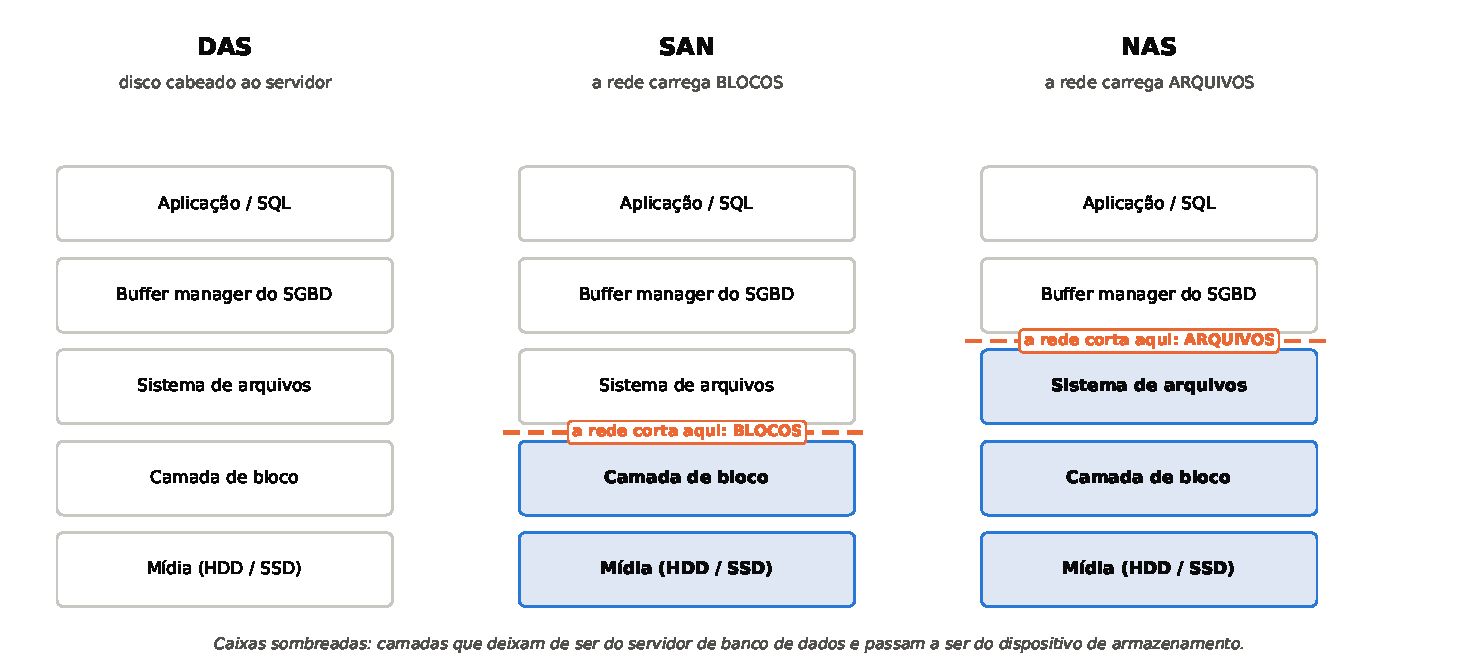
\includegraphics[width=0.96\textwidth]{fig/pilhas.pdf}
\caption{Onde a rede corta a pilha de E/S. Em DAS não há corte; em SAN o corte é abaixo do sistema
de arquivos (tráfego de blocos SCSI ou NVMe); em NAS o corte é acima (tráfego de operações de
arquivo). O componente sombreado é o que passa a ser responsabilidade do dispositivo de
armazenamento, e não mais do servidor de banco de dados.}
\label{fig:pilhas}
\end{figure}

%=====================================================================
\section{NAS --- \textit{Network Attached Storage}}
\label{sec:nas}
%=====================================================================

\subsection{Como funciona}

Elmasri e Navathe descrevem o NAS de maneira quase provocativa: os dispositivos NAS ``são, de
fato, servidores que não fornecem nenhum dos serviços comuns de servidor, mas simplesmente
permitem a adição de armazenamento para compartilhamento de arquivos''. Um único dispositivo de
\textit{hardware}, ``frequentemente chamado de \textit{NAS box} ou \textit{NAS head}, atua como a
interface entre o sistema NAS e os clientes de rede'', e ``os clientes se conectam ao \textit{NAS
head} em vez de aos dispositivos de armazenamento individuais'' \cite{elmasri2018}.

Operacionalmente, a sequência é a seguinte:

\begin{enumerate}[leftmargin=0.9cm,itemsep=2pt]
\item O \textit{NAS head} possui discos (ou SSDs) organizados internamente, tipicamente em RAID.
      Elmasri e Navathe registram que ``tais dispositivos tipicamente suportam RAID níveis 0, 1 e
      5'' \cite{elmasri2018}.
\item Sobre esse armazenamento, o \textit{NAS head} \textbf{monta e opera um sistema de arquivos
      próprio} (WAFL na NetApp, ZFS em muitos produtos, ext4/XFS em soluções abertas).
\item Esse sistema de arquivos é exportado pela LAN por meio de um protocolo de compartilhamento
      de arquivos --- SMB/CIFS, NFS ou AFP.
\item O cliente (o servidor de banco de dados) monta o compartilhamento e enxerga \emph{arquivos e
      diretórios}. Ele emite operações de arquivo (\textsc{open}, \textsc{read}, \textsc{write},
      \textsc{close}, \textsc{lock}), não comandos de bloco.
\end{enumerate}

O ponto que decide tudo está no item 2: \textbf{quem executa a alocação de blocos, o
\textit{journaling} de metadados e o controle de concorrência de arquivo é o dispositivo NAS,
não o servidor}. O servidor delega. Silberschatz resume: ``NAS é muito parecido com SAN, exceto
que, em vez de o armazenamento em rede aparecer como um disco grande, ele provê uma interface de
sistema de arquivos usando protocolos de sistema de arquivos em rede como NFS ou CIFS''
\cite{silberschatz2020}.

\subsection{Consequências diretas da semântica de arquivo}

\begin{itemize}[leftmargin=0.7cm,itemsep=3pt]
\item \textbf{Compartilhamento entre clientes é nativo.} Como o dispositivo é o dono do sistema de
      arquivos, ele arbitra o acesso concorrente. Vários servidores podem montar o mesmo
      compartilhamento sem \textit{software} adicional. Em SAN, dois servidores que montam o mesmo
      LUN com um sistema de arquivos comum destroem os dados, a menos que se use um sistema de
      arquivos de \textit{cluster} (GFS2, OCFS2, VMFS) ou um gerenciador de volume ciente de
      \textit{cluster}.
\item \textbf{Independência de sistema operacional do cliente.} Elmasri e Navathe: ``sistemas NAS
      alegam maior independência de sistema operacional dos clientes'' \cite{elmasri2018}.
\item \textbf{Coerência de \textit{cache} é o problema difícil.} O NFS não oferece coerência forte
      por padrão. O manual do Linux é explícito: ``o protocolo NFS não foi projetado para suportar
      coerência de \textit{cache} verdadeira de sistema de arquivos de \textit{cluster} sem algum
      tipo de serialização pela aplicação. Se coerência absoluta de \textit{cache} entre clientes
      for necessária, as aplicações devem usar travamento de arquivo'', e ``alternativamente, as
      aplicações podem abrir seus arquivos com a \textit{flag} \texttt{O\_DIRECT} para desabilitar
      completamente o \textit{cache} de dados'' \cite{nfsman}. Esta é exatamente a razão pela qual
      SGBDs suportados sobre NFS usam \texttt{O\_DIRECT} ou um cliente NFS próprio (ver
      Seção~\ref{sec:dnfs}).
\end{itemize}

%---------------------------------------------------------------------
\subsection{Protocolo NAS I --- SMB/CIFS}
\label{sec:smb}
%---------------------------------------------------------------------

\textbf{O que é.} SMB (\textit{Server Message Block}) é o protocolo de compartilhamento de
arquivos nativo do mundo Windows. CIFS (\textit{Common Internet File System}) \textbf{não é um
protocolo diferente}: é o nome que a Microsoft deu, em 1996, à família de dialetos hoje chamada
SMB~1. A documentação da própria Microsoft é explícita ao afirmar que o protocolo CIFS é um
\emph{dialeto} do SMB. Tratar ``SMB'' e ``CIFS'' como dois protocolos distintos é um erro comum; a
leitura correta é que \textbf{CIFS é SMB~1}, e que tudo posterior a isso se chama SMB~2 ou SMB~3.
O enunciado da tarefa usa a grafia composta ``SMB/CIFS'', que é a convenção da indústria e a
adotada aqui.

\textbf{Modelo.} É um protocolo de requisição-resposta orientado a sessão, historicamente sobre
NetBIOS (porta 139) e, desde o Windows 2000, diretamente sobre TCP na \textbf{porta 445}. As
operações são de alto nível: abrir arquivo, ler intervalo de \textit{bytes}, travar intervalo de
\textit{bytes}, enumerar diretório, consultar atributos.

\textbf{Evolução dos dialetos.} A Microsoft documenta as versões na especificação aberta
[MS-SMB2]. Os marcos relevantes:

\begin{table}[H]
\centering
\caption{Evolução dos dialetos SMB. Categoria de proveniência: documentação da Microsoft.}
\label{tab:smb}
{\footnotesize
\begin{tabular}{@{}llp{7.9cm}@{}}
\toprule
\textbf{Dialeto} & \textbf{Introduzido em} & \textbf{O que trouxe de relevante} \\
\midrule
SMB 1.0 (CIFS) & Anos 1980--1990 & Protocolo original; ``verboso'', muitas idas e voltas por
operação. \\
SMB 2.0 & Windows Vista / Server 2008 & Reescrita: conjunto de comandos reduzido, requisições
compostas, créditos de fluxo, identificadores de 64 bits. \\
SMB 2.1 & Windows 7 / Server 2008 R2 & \textit{Leasing} de arquivo (\textit{cache} de cliente mais
agressivo e correto). \\
SMB 3.0 & Windows 8 / Server 2012 & \textbf{SMB Direct} (RDMA), \textbf{SMB Multichannel},
\textit{transparent failover}, compartilhamentos continuamente disponíveis, criptografia
fim-a-fim (\textbf{AES-128-CCM}). É a versão que torna SMB viável para banco de dados. \\
SMB 3.0.2 & Windows 8.1 / Server 2012 R2 & Otimizações de E/S pequena e aleatória; possibilidade
de remover SMB1 completamente. \\
SMB 3.1.1 & Windows 10 / Server 2016 & Negociação pré-autenticação com integridade protegida;
criptografia \textbf{AES-128-GCM} (AES-256-GCM só a partir do Windows 11 / Server 2022). \\
\bottomrule
\end{tabular}}
\end{table}

\textbf{Estado do SMB 1.} A Microsoft documenta que ``a partir do \textit{Windows 10 Fall Creators
Update} e do Windows Server 2019, o SMBv1 não é mais instalado por padrão'', e que ``o SMBv1 não é
instalado por padrão em nenhuma edição do Windows 11 ou do Windows Server 2019 e versões
posteriores'' \cite{mssmb1}. \textbf{Precisão de rótulo:} o primeiro \emph{Windows Server} sem SMBv1
por padrão foi a versão 1709 do canal semianual; o Server 2019 é o primeiro do canal de suporte
prolongado (LTSC). \textbf{Consequência prática para NAS:} equipamentos antigos que só
falam CIFS/SMB1 deixam de ser montáveis por clientes modernos sem reabilitação manual de um
protocolo com vulnerabilidades conhecidas. Ao citar ``SMB/CIFS'' num projeto novo em 2026, o que
se está de fato especificando é SMB~3.

\textbf{Uso com SGBD.} A Microsoft suporta oficialmente colocar arquivos de banco de dados do SQL
Server em compartilhamento SMB: ``o SQL Server 2012 (11.x) e versões posteriores'' suportam
armazenar bancos de dados de sistema (\texttt{master}, \texttt{model}, \texttt{msdb},
\texttt{tempdb}) e de usuário em \textit{fileshare} SMB, tanto em instalação isolada quanto em
\textit{failover cluster} \cite{mssqlsmb}. As condições que a documentação impõe são instrutivas
porque expõem exatamente os pontos frágeis do NAS para banco de dados:

\begin{itemize}[leftmargin=0.7cm,itemsep=2pt]
\item para cargas críticas, ``o compartilhamento de arquivos deve suportar \textit{SMB 3.0
      transparent failover} (disponibilidade contínua)'' \cite{mssqlsmb} --- isto é: o protocolo
      precisa sobreviver à troca de nó do servidor de arquivos sem devolver erro ao SGBD;
\item a conta de serviço precisa de \texttt{FULL CONTROL} no compartilhamento e no NTFS;
\item \textbf{FILESTREAM não é suportado} em compartilhamento SMB;
\item caminhos de \textit{loopback}, compartilhamentos administrativos (\texttt{\textbackslash\textbackslash
      servidor\textbackslash x\$}) e unidades mapeadas não são suportados --- só caminhos UNC.
\end{itemize}

%---------------------------------------------------------------------
\subsection{Protocolo NAS II --- NFS}
\label{sec:nfs}
%---------------------------------------------------------------------

\textbf{O que é.} O NFS (\textit{Network File System}) é o padrão aberto de compartilhamento de
arquivos do mundo UNIX/Linux, originalmente da Sun Microsystems (1984) e hoje mantido pelo IETF.
É o protocolo NAS que efetivamente aparece em instalações sérias de banco de dados.

\textbf{Versões e o que muda em cada uma.} A Tabela~\ref{tab:nfs} traz a linha do tempo com as
normas. Proveniência: RFCs do IETF (especificação normativa).

\begin{table}[H]
\centering
\caption{Versões do NFS. Fonte: RFCs do IETF. \textbf{Atenção à leitura:} a coluna
``norma vigente'' traz a RFC \emph{atualmente em vigor}, que muitas vezes é uma reedição posterior
--- por isso a v4.2 (2016) aparece com data anterior à da v4.1 (2020). A cronologia real do
protocolo está na coluna ``introduzida em''.}
\label{tab:nfs}
{\footnotesize
\begin{tabular}{@{}llll@{}}
\toprule
\textbf{Versão} & \makecell[l]{\textbf{Introduzida}\\\textbf{em}} & \makecell[l]{\textbf{Norma}\\\textbf{vigente}} & \textbf{Característica determinante} \\
\midrule
NFSv2 & 1989 & RFC 1094 & \parbox[t]{7.3cm}{\raggedright Sobre UDP; \textit{offsets} de 32 bits (limite de 2~GiB por arquivo).\strut} \\
\addlinespace
NFSv3 & 1995 & RFC 1813 & \parbox[t]{7.3cm}{\raggedright \textit{Offsets} de 64 bits, escritas assíncronas com
\textsc{commit} explícito, TCP. \textbf{Sem estado}: o travamento fica \emph{fora} do protocolo, num
serviço separado (NLM, \textit{Network Lock Manager}), o que torna a recuperação após falha frágil.\strut} \\
\addlinespace
NFSv4.0 & \makecell[l]{2000\\(RFC 3010)} & \makecell[l]{RFC 7530\\(2015)} & \parbox[t]{7.3cm}{\raggedright \textbf{Com estado}. Travamento, montagem e
ACLs integrados ao protocolo; operações compostas (\textsc{compound}) reduzem idas e voltas; uma
única porta (\textbf{2049}), o que o torna atravessável por \textit{firewall}; segurança via
RPCSEC\_GSS.\strut} \\
\addlinespace
NFSv4.1 & \makecell[l]{2010\\(RFC 5661)} & \makecell[l]{RFC 8881\\(2020)} & \parbox[t]{7.3cm}{\raggedright Modelo de \textbf{sessões}, que dá semântica de
execução \textbf{exatamente uma vez} (\textit{exactly-once semantics}): a garantia vem do par sessão
$+$ \textit{reply cache} e vale para requisições \textsc{compound} precedidas de uma operação
\textsc{sequence} (ou \textsc{cb\_sequence}) --- não é incondicional. E \textbf{pNFS}
(\textit{parallel NFS}), que separa o caminho de metadados do caminho de dados, permitindo que o
cliente leia dados diretamente de vários servidores em paralelo \cite{rfc8881}.\strut} \\
\addlinespace
NFSv4.2 & 2016 & RFC 7862 & \parbox[t]{7.3cm}{\raggedright Cópia no lado do servidor, arquivos esparsos,
\textit{hole punching}.\strut} \\
\bottomrule
\end{tabular}}
\end{table}

\correcao{Correção de rótulo: RFC 8881 obsoleta a RFC 5661}{%
Boa parte da literatura ainda cita a RFC 5661 (2010) como a especificação do NFSv4.1. Ela foi
\textbf{obsoletada pela RFC 8881, de 2020} \cite{rfc8881}. Citar a RFC 5661 hoje aponta para um
documento superado --- ainda que o conteúdo técnico seja em grande parte o mesmo, a referência
correta é a RFC 8881.}

\textbf{O calcanhar de Aquiles: coerência de \textit{cache}.} O NFS implementa
\textit{close-to-open consistency}: o cliente verifica a validade do \textit{cache} ao abrir o
arquivo e descarrega as alterações pendentes ao fechá-lo \cite{nfsman}. Isso é adequado para
arquivos de escritório e desastroso para um arquivo de dados de banco aberto por semanas sem nunca
ser fechado. É por isso que todo SGBD suportado sobre NFS ou usa \texttt{O\_DIRECT}, ou substitui o
cliente NFS do sistema operacional pelo seu próprio.

\textbf{Oracle Direct NFS (dNFS).}
\label{sec:dnfs}
A Oracle escolheu o caminho radical: ``o cliente Direct NFS (dNFS) integra a funcionalidade de
cliente NFS diretamente no \textit{software} Oracle para otimizar o caminho de E/S entre a Oracle e
o servidor NFS'' \cite{oracledn}. Ou seja, o SGBD implementa NFS \emph{dentro de si mesmo}, falando
diretamente com o servidor NFS por \textit{sockets} próprios e ignorando o cliente NFS do
\textit{kernel}. Isso lhe dá controle sobre profundidade de fila, número de conexões TCP e
semântica de \textit{cache}. A Oracle documenta que ``o cliente Direct NFS suporta os protocolos
NFSv3, NFSv4, NFSv4.1 e pNFS'', e que ``se o Oracle Database não conseguir se conectar a um
servidor NFS usando o cliente Direct NFS, então ele se conecta usando o cliente NFS do
\textit{kernel} do sistema operacional'' \cite{oracledn}.

\destaque{Por que o dNFS importa para o argumento deste trabalho}{%
A existência do dNFS é a melhor evidência empírica da tese central: NAS entrega uma abstração
\emph{alta demais} para um SGBD. O maior fornecedor de bancos de dados relacionais do mercado
achou necessário reimplementar o protocolo NAS dentro do próprio motor para poder usá-lo. Isso não
significa que NAS não sirva para banco --- significa que serve \emph{quando o motor participa da
decisão}, não quando ele é tratado como uma aplicação qualquer.}

%---------------------------------------------------------------------
\subsection{Protocolo NAS III --- AFP (\textit{Apple Filing Protocol})}
\label{sec:afp}
%---------------------------------------------------------------------

\textbf{O que é.} O AFP é o protocolo proprietário de compartilhamento de arquivos da Apple,
originado no \textit{AppleTalk Filing Protocol} de 1985--1988. Sua característica distintiva era
preservar corretamente as particularidades do sistema de arquivos do Macintosh --- \textit{resource
forks}, tipo e criador de arquivo, nomes longos com acentuação, e metadados que o SMB1 da época
mutilava. Por muitos anos foi o único jeito de fazer um NAS servir Macs sem corromper arquivos, e
era o protocolo obrigatório para \textit{backups} do Time Machine em rede.

\textbf{Como funciona.} O AFP é um protocolo de sessão, com estado, historicamente transportado
sobre AppleTalk (ASP/ATP) e, desde o AFP 3.0, sobre TCP na \textbf{porta 548} por meio do
\textbf{DSI} (\textit{Data Stream Interface}), a camada que enquadra requisições e respostas e
multiplexa comandos numa conexão TCP. Suas características determinantes, e o que elas explicam:

\begin{itemize}[leftmargin=0.7cm,itemsep=2pt]
\item \textbf{Modelo de sessão com estado.} O cliente faz \textsc{FPLogin}, abre um \textit{volume}
      com \textsc{FPOpenVol}, e daí em diante opera sobre identificadores de sessão. Falha de rede
      derruba a sessão; o AFP 3.x acrescentou reconexão para mitigar isso.
\item \textbf{Bifurcação de arquivo (\textit{forks}).} O AFP foi desenhado em torno do sistema de
      arquivos do Macintosh, em que um arquivo tem um \textit{data fork} e um \textit{resource
      fork} --- e os comandos são explicitamente bifurcados: \textsc{FPOpenFork},
      \textsc{FPRead}/\textsc{FPWrite} sobre um \textit{fork} identificado. Era esta a razão
      técnica de existir: SMB1 e NFS não tinham como representar o \textit{resource fork} sem
      truques (arquivos \texttt{.\_nome}, \textit{AppleDouble}), e o resultado era corrupção
      silenciosa de metadados.
\item \textbf{Metadados nativos do Mac} --- tipo e criador de arquivo, \textit{Finder info},
      posição de ícone --- transportados como atributos de primeira classe, não como emulação.
\item \textbf{Travamento por intervalo de \textit{bytes}} via \textsc{FPByteRangeLock}, mas com
      semântica de sessão: o travamento morre com a sessão, e não há o equivalente às
      \textit{leases} com prazo do NFSv4 ou aos \textit{oplocks}/\textit{leases} do SMB~2/3.
\item \textbf{Nomes e codificação:} suporte nativo a nomes longos em UTF-8 com decomposição
      canônica (a forma NFD que o macOS usa), outro ponto em que os protocolos concorrentes da época
      falhavam.
\end{itemize}

\textbf{O que ele nunca teve} --- e que é a razão de não servir a banco de dados: nenhum caminho de
dados com RDMA, nenhum equivalente a \textit{multichannel}, nenhuma noção de disponibilidade
contínua com \textit{failover} transparente, e um travamento amarrado à sessão. Comparado ao SMB~3
(Seção~\ref{sec:smb}) e ao NFSv4.1 (Seção~\ref{sec:nfs}), o AFP parou no conjunto de recursos de um
protocolo de compartilhamento de arquivos de escritório.

\textbf{Estado atual --- e é aqui que a maior parte do material disponível erra.} O AFP está em
processo de remoção do macOS, em duas etapas separadas por cerca de cinco anos:

\begin{itemize}[leftmargin=0.7cm,itemsep=2pt]
\item o \textbf{servidor} AFP (a capacidade de um Mac \emph{compartilhar} pastas por AFP) foi
      removido no macOS 11 Big Sur (2020);
\item o \textbf{cliente} AFP (a capacidade de um Mac \emph{montar} um compartilhamento AFP de um
      NAS) foi \textbf{depreciado no macOS 15.5 Sequoia}, em maio de 2025. O texto da Apple é
      direto: ``o cliente do \textit{Apple Filing Protocol} (AFP) está depreciado e será removido em
      uma versão futura do macOS'' \cite{appleafp};
\item para o \textbf{macOS 27}, a Apple informa oficialmente que o Time Machine deixa de
      suportar destinos AFP, incluindo Time Capsules e AirPort Disks \cite{appleafptm}.
\end{itemize}

\correcao{Armadilha de rótulo: cliente $\neq$ servidor --- e correção da nossa própria primeira versão}{%
Dizer ``a Apple removeu o AFP no Big Sur'' é meia-verdade que erra por cinco anos: removeu o
\emph{servidor}; o \emph{cliente} sobreviveu até 2026.

\smallskip
\textbf{Registro de erro nosso.} A primeira versão deste relatório afirmava que ``a versão de
remoção efetiva ainda não foi anunciada''. Isso era verdade em maio de 2025 e \textbf{já não era
verdade em setembro de 2026}: a rodada de verificação adversarial (Seção~\ref{sec:adversarial})
localizou a documentação oficial atualizada em julho de 2026 sobre o fim do suporte a
destinos AFP do Time Machine no macOS~27 \cite{appleafptm}.

\smallskip
\textbf{Ressalva de alcance:} a fonte oficial confirma o fim do suporte do Time Machine a
destinos AFP; não usamos isso para afirmar além do que a Apple documenta sobre todo cliente AFP.
A depreciação do cliente permanece documentada separadamente \cite{appleafp}.}

\textbf{Relevância para SBD: nenhuma, e isso é o achado.} \textbf{Alcance da afirmação:} pesquisamos
as matrizes de suporte publicadas por Oracle, Microsoft, PostgreSQL e MySQL e não localizamos AFP em
nenhuma delas; o que afirmamos, portanto, é que \emph{nenhum dos quatro SGBDs de maior participação
o lista como configuração suportada}, e não um negativo universal sobre todo o mercado. O motivo
técnico está na Seção anterior: sem travamento independente de sessão, sem RDMA e sem
disponibilidade contínua, o AFP não atende aos requisitos 4 e 5 da Seção~\ref{sec:engine}. O protocolo nunca teve travamento em intervalo de \textit{bytes} adequado a
cargas transacionais, nunca teve RDMA nem múltiplos canais, e agora chegou ao fim da vida. A
recomendação técnica correta, em 2026, é: \textbf{para um NAS que precise servir clientes Apple,
use SMB~3}, que é o protocolo primário do macOS desde o OS~X 10.9 Mavericks (2013) --- a transição
já tinha treze anos quando o AFP foi finalmente retirado. Se o AFP aparece na lista do enunciado, é
como item de completude histórica; é mais honesto dizer isso do que fabricar uma aplicação de banco
de dados para ele.

\subsection{Vantagens e desvantagens do NAS}
\label{sec:vantnas}

\correcao{Declaração de lacuna: os itens de custo desta tabela não têm número}{%
As linhas de custo da Tabela~\ref{tab:vantnas} e das tabelas comparativas seguintes --- ``menor
custo por TB útil'', ``custo relativo menor/maior'' --- são \textbf{afirmações estruturais, não
medições}. Elas se sustentam em um fato verificável (o NAS dispensa HBA, \textit{switch} FC,
transceptores e cabeamento dedicados, que a SAN exige) e em outro que \emph{não} conseguimos
sustentar com fonte: \emph{quanto} isso representa em US\$/TB útil.

\smallskip
Aplicando a regra da Seção~\ref{sec:metodologia}, a categoria correta é \textbf{não encontrado}.
Não localizamos, para nenhum fornecedor, tabela pública de preço de porta FC ou de \textit{array}
unificado que permitisse uma comparação honesta e datada --- preço de canal depende de volume e de
contrato, e reproduzi-lo sem data seria violar a regra de que ``número volátil sem data não é
dado''.

\smallskip
\textbf{O que se pode afirmar com rigor, e é o que afirmamos:} a SAN acrescenta \emph{categorias} de
componente que o NAS não tem, e cada categoria acrescenta custo de aquisição, de manutenção e de
competência da equipe. A \emph{direção} da comparação é estrutural e certa; a \emph{magnitude} não
está neste trabalho. O Apêndice de aprofundamentos registra o levantamento de TCO como o item que
fecharia essa lacuna.}

\begin{table}[H]
\centering
\caption{NAS: vantagens e desvantagens sob a ótica de um SBD. \textbf{As linhas de custo são
qualitativas} --- ver a declaração de lacuna acima.}
\label{tab:vantnas}
{\footnotesize
\begin{tabular}{@{}p{7.4cm}p{7.4cm}@{}}
\toprule
\textbf{Vantagens} & \textbf{Desvantagens} \\
\midrule
Usa a rede Ethernet/IP existente: sem HBA dedicada, sem \textit{switch} FC, sem equipe
especializada. & Compete por banda com o tráfego de aplicação, a menos que se segregue por VLAN ou
rede física separada. \\
Compartilhamento concorrente entre servidores é nativo, sem sistema de arquivos de
\textit{cluster}. & Coerência de \textit{cache} fraca por padrão (\textit{close-to-open}); exige
\texttt{O\_DIRECT}, travamento explícito ou cliente dedicado \cite{nfsman}. \\
Provisionamento simples: criar um compartilhamento e conceder permissão, sem zoneamento nem
mapeamento de LUN. & Camada extra de sistema de arquivos no caminho: metadados, travamento e
\textit{journaling} do lado do NAS somam latência. \\
Independência de sistema operacional dos clientes \cite{elmasri2018}. & Semântica de escrita
atômica de página não é garantida pelo protocolo; o SGBD tem que se proteger sozinho. \\
Instantâneos, \textit{clones} e replicação no nível de arquivo, com granularidade compreensível. &
Nem todo recurso do SGBD funciona (FILESTREAM não é suportado sobre SMB \cite{mssqlsmb}). \\
Custo por terabyte útil menor, tanto de aquisição quanto de operação. & Depende de recursos
avançados do protocolo (SMB 3 \textit{transparent failover}, NFSv4.1 \textit{sessions}) para
sobreviver a falhas sem derrubar a instância. \\
\bottomrule
\end{tabular}}
\end{table}

%=====================================================================
\section{SAN --- \textit{Storage Area Network}}
\label{sec:san}
%=====================================================================

\subsection{Como funciona}

Silberschatz define com precisão: ``na arquitetura de rede de área de armazenamento (SAN), um
grande número de discos é conectado por uma rede de alta velocidade a um conjunto de computadores
servidores. Os discos são geralmente organizados localmente usando uma técnica de organização de
armazenamento chamada RAID, para dar aos servidores uma \emph{visão lógica de um disco muito
grande e muito confiável}'' \cite{silberschatz2020}. Elmasri e Navathe complementam com a
motivação operacional: ``em uma SAN, os periféricos de armazenamento \textit{online} são
configurados como nós em uma rede de alta velocidade e podem ser conectados e desconectados de
servidores de maneira muito flexível'' \cite{elmasri2018}.

A sequência operacional, em contraste direto com a do NAS:

\begin{enumerate}[leftmargin=0.9cm,itemsep=2pt]
\item O \textit{array} de armazenamento agrega discos físicos em \textit{pools} protegidos por
      RAID ou por codificação de apagamento.
\item Do \textit{pool}, o administrador recorta volumes lógicos e os apresenta como \textbf{LUNs}
      (\textit{Logical Unit Numbers}) --- o identificador SCSI de uma unidade lógica.
\item Uma rede dedicada (FC ou Ethernet segregada) transporta \textbf{comandos SCSI} (ou, mais
      recentemente, comandos NVMe) entre o iniciador no servidor e o alvo no \textit{array}.
\item O sistema operacional do servidor vê um \textbf{dispositivo de bloco cru}, indistinguível de
      um disco local: \texttt{/dev/sdb}, \texttt{PhysicalDrive2}. Ele formata esse dispositivo com
      seu próprio sistema de arquivos, ou o entrega cru ao SGBD (é o que o Oracle ASM faz).
\end{enumerate}

A frase de Elmasri e Navathe que melhor captura o efeito é: ``aplicações de gerenciamento de
armazenamento existentes podem ser portadas para configurações SAN usando redes \textit{Fibre
Channel} que encapsulam o protocolo SCSI legado. Como resultado, \textbf{os dispositivos ligados à
SAN aparecem como dispositivos SCSI}'' \cite{elmasri2018}. É uma ilusão deliberada, e é ela que faz
a SAN funcionar: o servidor e o SGBD não precisam saber que existe uma rede no caminho.

\subsection{\textit{Fibre Channel}: a pilha}
\label{sec:fc}

O \textit{Fibre Channel} é padronizado pelo comitê \textbf{T11} do INCITS. Uma observação de
nomenclatura que vale registrar: a grafia normativa é \textbf{\textit{Fibre}} Channel, com
\textit{-re}, justamente para deixar claro que o padrão não exige fibra óptica --- as primeiras
variantes rodavam sobre cabo de cobre. O enunciado da tarefa escreve ``FC (Fibre/Fiber Channel)'',
reconhecendo as duas grafias; o livro do Elmasri alterna entre ``Fibre Channel'' e ``Fiber
Channel'' no mesmo capítulo \cite{elmasri2018}, e o do Silberschatz usa ``Fiber Channel FC''
\cite{silberschatz2020}. A grafia do T11 é \textit{Fibre}.

A pilha FC é dividida em cinco camadas:

\begin{table}[H]
\centering
\caption{Camadas do \textit{Fibre Channel}. Proveniência: arquitetura T11/INCITS.}
\label{tab:fclayers}
{\footnotesize
\begin{tabular}{@{}llp{9.1cm}@{}}
\toprule
\textbf{Camada} & \textbf{Nome} & \textbf{Função} \\
\midrule
FC-0 & Físico & Meio, conectores, transceptores, taxa de sinalização (\textit{baud}). \\
FC-1 & Codificação & Codificação de linha e sincronismo: \textbf{8b/10b} até 8GFC;
\textbf{64b/66b} no 16GFC; \textbf{256b/257b com RS-FEC obrigatório} a partir de 32GFC
(RS(528,514) no 32GFC); sinalização \textbf{PAM-4} a partir de 64GFC. \\
FC-2 & Sinalização & \textbf{Camada central}: quadros, sequências, trocas
(\textit{exchanges}), classes de serviço e o \textbf{controle de fluxo por créditos de
\textit{buffer}} (BB\_Credit). \\
FC-3 & Serviços comuns & Serviços que atravessam múltiplas portas (\textit{hunt groups},
\textit{striping}). Pouco usada. \\
FC-4 & Mapeamento & Mapeia protocolos superiores sobre FC. O relevante aqui é o \textbf{FCP}
(\textit{Fibre Channel Protocol}), o mapeamento de SCSI-3 sobre FC; e, mais recentemente,
\textbf{FC-NVMe}. \\
\bottomrule
\end{tabular}}
\end{table}

\textbf{Por que o controle de fluxo por créditos importa.} Diferente do Ethernet clássico, que
descarta quadros sob congestionamento e delega a recuperação ao TCP, o FC-2 usa
\textbf{BB\_Credit}: uma porta só transmite um quadro se tiver crédito, e o crédito é devolvido
pela porta receptora quando ela libera um \textit{buffer}. O resultado é uma rede
\emph{sem perdas por congestionamento}, e é isso que permite ao FC dispensar TCP e ainda assim
entregar comandos SCSI de forma confiável. Como referência de magnitude, o \textit{product brief}
do \textit{switch} Brocade G710 declara ``2000 \textit{buffers} de quadro alocados dinamicamente''
\cite{brocadeg710}. \textbf{Proveniência:} \textit{datasheet} de fabricante, modelo específico.

\textbf{Endereçamento e zoneamento.} Cada porta FC tem um \textbf{WWN} (\textit{World Wide Name}),
identificador global de 64 bits gravado de fábrica, análogo ao endereço MAC. Ao entrar na
\textit{fabric}, a porta faz \textsc{flogi} e recebe um \textbf{endereço de \textit{fabric} de 24
bits} (Domain / Area / Port), usado para roteamento. O \textbf{zoneamento} (\textit{zoning}),
configurado no \textit{switch}, define quais iniciadores podem ver quais alvos; é o controle de
acesso da SAN, e o análogo funcional do \textit{firewall} na rede IP. Complementarmente, o
\textbf{LUN masking}, configurado no \textit{array}, define quais LUNs cada iniciador enxerga. As
duas camadas juntas são o que impede que o servidor de teste monte, por engano, o LUN de produção.

\subsubsection*{Velocidades: onde mora a armadilha de rótulo}

Há duas maneiras de expressar a velocidade de um enlace FC, e confundi-las é a origem da maior
parte dos erros que circulam sobre desempenho de \textit{Fibre Channel}. A
Tabela~\ref{tab:fcspeed} reproduz o \textit{roadmap} vigente da FCIA, que desde a revisão de 2023
publica \textbf{duas tabelas separadas}: o FC serial (uma via) e o \textit{Inter-Switch Link}
(vias paralelas) \cite{fciaroadmap}.

\begin{table}[H]
\centering
\caption{\textit{Speedmap} vigente do \textit{Fibre Channel} \cite{fciaroadmap}. As colunas
``FCIA'', ``taxa de linha'', ``T11'' e ``mercado'' são reproduzidas da fonte; a coluna ``por
direção'' é \textbf{derivação nossa} (metade do valor da FCIA), justificada logo abaixo.
``Demanda'' $=$ ``\textit{market demand}'' no original.}
\label{tab:fcspeed}
{\footnotesize
\begin{tabular}{@{}lrrlcc@{}}
\toprule
\textbf{Produto} & \makecell[r]{\textbf{FCIA}\\\textbf{(MB/s)}} &
\makecell[r]{\textbf{Por direção}\\\textbf{(MB/s, derivado)}} &
\makecell[c]{\textbf{Taxa de linha}\\\textbf{(GBd)}} &
\makecell[c]{\textbf{Norma T11}\\\textbf{concluída}} &
\makecell[c]{\textbf{Disponib.}\\\textbf{no mercado}} \\
\midrule
\multicolumn{6}{@{}l}{\textit{\textbf{Fibre Channel serial}}}\\
8GFC   & 1.600  & 800    & 8,5 NRZ      & 2006 & 2008 \\
16GFC  & 3.200  & 1.600  & 14,025 NRZ   & 2009 & 2011 \\
32GFC  & 6.400  & 3.200  & 28,05 NRZ    & 2013 & 2016 \\
64GFC  & 12.800 & 6.400  & 28,9 PAM-4   & 2017 & 2020 \\
\textbf{128GFC} & \textbf{24.850} & \textbf{12.425} & \textbf{56,1 PAM-4} & \textbf{2022} & \textbf{2024} \\
256GFC & 49.700 & 24.850 & 112,2 PAM-4  & 2025 & demanda \\
512GFC & TBD    & TBD    & TBD          & 2029 & demanda \\
1TFC   & TBD    & TBD    & TBD          & 2033 & demanda \\
\addlinespace
\multicolumn{6}{@{}l}{\textit{\textbf{Inter-Switch Link} (vias paralelas)}}\\
10GFC  & 2.400  & 1.200  & 10,52 NRZ        & 2003 & 2009 \\
128GFC & 25.600 & 12.800 & 4 $\times$ 28,05 NRZ  & 2014 & 2016 \\
256GFC & 51.200 & 25.600 & 4 $\times$ 28,9 PAM-4 & 2018 & 2020 \\
\bottomrule
\end{tabular}}
\end{table}

\destaque{Prova de que os números da FCIA são \textit{full-duplex} --- e ela é de física, não de opinião}{%
A FCIA \textbf{não declara} se seus valores são por direção ou somados. A única nota de rodapé do
\textit{roadmap} diz: ``estes números são representativos de valores de vazão para a taxa de linha e
dependem da carga útil'' \cite{fciaroadmap}. \textbf{Portanto, ler os valores como
\textit{full-duplex} é derivação nossa, não citação} --- e é assim que apresentamos. A prova, porém,
é dedutiva e não admite discussão: \emph{uma direção não pode transportar mais bits do que a linha
sinaliza}.

\smallskip
\textbf{16GFC.} A FCIA publica 3.200 MB/s $= 3.200 \times 8 = \mathbf{25{,}6}$~Gb/s. A taxa de
linha é 14,025 GBd em NRZ, isto é, \textbf{14,025 Gb/s brutos}. Como $25{,}6 > 14{,}025$, o valor
publicado \emph{não cabe} numa única direção.

\smallskip
\textbf{128GFC.} A FCIA publica 24.850 MB/s $= \mathbf{198{,}8}$~Gb/s. A linha é 56,1 GBd em PAM-4
(2 bits por símbolo) $= \mathbf{112{,}2}$~Gb/s brutos. Como $198{,}8 > 112{,}2$, idem.

\smallskip
Em ambos os casos o valor publicado excede a capacidade bruta da linha por um fator próximo de
dois. \textbf{A única leitura fisicamente possível é a soma dos dois sentidos.}
\textbf{Consequência prática:} ao dimensionar o caminho de E/S de um SGBD, use a coluna ``por
direção'' --- a leitura de um \textit{tablespace} e a escrita do WAL não se somam num único sentido.
Usar o número da FCIA sem dividir por dois superdimensiona o enlace em 100\%.}

\correcao{O achado: a convenção de nomenclatura \emph{quebra} na Gen 8, e há \textbf{três} números
chamados ``128GFC''}{%
Até o 64GFC vale uma regra simples e muito repetida: \textbf{$X$ GFC entrega $X \times 100$ MB/s por
direção} --- 16GFC $\rightarrow$ 1.600; 32GFC $\rightarrow$ 3.200; 64GFC $\rightarrow$ 6.400. Nessas
gerações a razão entre o valor da FCIA e o da convenção é \textbf{exatamente 2,00}.

\smallskip
\textbf{Na geração 8 a regra falha}, e o motivo está documentado pela própria FCIA: ``dobrar a
velocidade teria exigido uma taxa de linha de 115,6 Gb/s, e as equipes técnicas não julgaram
viável fechar o \textit{link budget}'' \cite{fcia128}. A linha ficou em \textbf{112,2 Gb/s}, e não
nos 115,6 que o nome ``128'' sugere. Logo:
\[
24.850 \div 2 = \mathbf{12.425}\ \text{MB/s por direção} \;\neq\; 12.800\ \text{que o nome implica};
\qquad \frac{24.850}{12.800} = 1{,}941 \neq 2.
\]

\smallskip
\textbf{Derivação nossa que confirma a leitura.} A eficiência útil sobre a linha bruta é a mesma nas
duas gerações PAM-4: no 64GFC, $6.400\ \text{MB/s} = 51{,}2$~Gb/s sobre 57,8 brutos $= 88{,}6\%$; no
128GFC, $12.425\ \text{MB/s} = 99{,}4$~Gb/s sobre 112,2 brutos $= 88{,}6\%$. E a razão entre as
vazões, $24.850/12.800 = 1{,}941$, é \emph{idêntica} à razão entre as taxas de linha,
$56{,}1/28{,}9 = 1{,}941$. \textbf{A FCIA escalou o 128GFC a partir do 64GFC pela taxa de linha}; o
nome é que arredondou para cima.

\smallskip
\textbf{Resultado: três números diferentes atendem por ``128GFC''.}
\begin{itemize}[leftmargin=0.7cm,itemsep=1pt,topsep=2pt]
\item \textbf{25.600 MB/s} --- o 128GFC de \textit{Inter-Switch Link}, quatro vias de 28,05 GBd NRZ.
      Esse, sim, soma 128 Gb/s de vias, e é de 2016.
\item \textbf{24.850 MB/s} --- o 128GFC serial de Gen 8, uma via de 56,1 GBd PAM-4, de 2024. É o que
      se compra hoje como ``128GFC''.
\item \textbf{12.800 MB/s} --- o valor que a norma FC-PI-8 rev.\ 1.4 ainda publica como
      \textit{Data Rate}. A FCIA registra, no seu Q\&A, a pergunta ``isso mudou?'' e a resposta:
      ``decidimos não mudar isso no documento FC'' \cite{fcia128}. É um valor \textbf{herdado da
      convenção de nomenclatura}, deliberadamente não atualizado.
\end{itemize}

\textbf{Quem cita ``128GFC'' sem dizer qual dos três está citando erra por até $2\times$.}}

\correcao{Registro de erro nosso, e do que ele custou}{%
A primeira versão deste relatório publicava o \textit{speedmap} \textbf{v21, de dezembro de 2016}
\cite{fciaspeedmap},
e declarava não ter conseguido acessar a tabela numérica vigente. \textbf{As duas coisas estavam
erradas:} a tabela v24 (jul./2023) está disponível em HTML na página de \textit{roadmap} da FCIA
\cite{fciaroadmap}, e com ela vieram três correções --- a separação entre FC serial e ISL, a
disponibilidade do 64GFC em 2020 (e não 2019), e sobretudo o 128GFC serial de 24.850 MB/s, que
\emph{refuta} a afirmação de ``fator exatamente 2'' que aquela versão trazia como conclusão.

\smallskip
\textbf{Por que registramos isso em vez de apagar.} Declarar uma lacuna é resultado legítimo
(Seção~\ref{sec:metodologia}) --- \emph{declarar uma lacuna que não existe é o oposto disso}, e
contamina todas as outras declarações de lacuna do trabalho. O erro foi encontrado na segunda
rodada de verificação adversarial (Seção~\ref{sec:adversarial2}) e é o mais grave que cometemos.}

\correcao{Conferindo o Silberschatz contra a tabela}{%
Silberschatz \textit{et al.} escrevem que o \textit{Fibre Channel} ``suporta taxas de transferência
de 1,6 a 12 \textit{gigabytes} por segundo, dependendo da versão'' \cite{silberschatz2020}.
Confrontando com a Tabela~\ref{tab:fcspeed}: 1,6 GB/s $=$ 1.600 MB/s $=$ 16GFC \emph{por direção}; e
12 GB/s $\approx$ 12.800 MB/s $=$ o valor \emph{full-duplex} do 64GFC --- ou, equivalentemente, o
número herdado que o FC-PI-8 publica para o 128GFC. \textbf{A faixa do livro está correta para as
gerações disponíveis quando a edição foi escrita}; o que ela não diz é qual das duas escalas está
usando, e um leitor que a compare com o \textit{speedmap} vai achar que o livro errou por um fator
de 2. Registramos como \emph{ambiguidade de rótulo}, não como erro. O erro de fato, no mesmo
parágrafo, é outro, e está na Seção~\ref{sec:correcoes}.}


\subsection{Topologias FC --- incluindo o ``FC \textit{Switch}'' do enunciado}
\label{sec:topologias}

O enunciado lista ``FC \textit{Switch}'' como uma das variações a discutir. Tecnicamente,
\textit{FC Switch} não é um protocolo, e sim uma das três \textbf{topologias} definidas pelo T11.
Elmasri e Navathe as descrevem como as ``alternativas arquiteturais atuais para SAN''
\cite{elmasri2018}:

\begin{table}[H]
\centering
\caption{Topologias \textit{Fibre Channel}.}
\label{tab:topologias}
{\footnotesize
\begin{tabular}{@{}lp{11.2cm}@{}}
\toprule
\textbf{Topologia} & \textbf{Descrição e situação atual} \\
\midrule
\textbf{Ponto-a-ponto} (FC-P2P) & Dois dispositivos ligados diretamente, sem \textit{switch}. Banda
integralmente dedicada, mas conectividade de dois nós apenas. Elmasri e Navathe a listam como a
alternativa mais simples: ``conexões ponto-a-ponto entre servidores e sistemas de armazenamento via
\textit{Fibre Channel}'' \cite{elmasri2018}. Uso residual: ligação direta de um servidor a um
\textit{array}. \\
\addlinespace
\textbf{\textit{Arbitrated loop}} (FC-AL) & Até 126 dispositivos-nó (NL\_Ports) mais uma FL\_Port,
totalizando 127 endereços de anel, com arbitragem pelo direito de transmitir. \textbf{Banda compartilhada}: um dispositivo lento degrada
todos, e a inserção de um nó reinicializa o anel (LIP), causando pausas de E/S. Foi a topologia dos
\textit{hubs} FC dos anos 1990 e das gavetas de disco FC-AL. \textbf{Está obsoleta} --- não há
produto novo de SAN sendo construído sobre ela. \\
\addlinespace
\textbf{\textit{Switched fabric}} (FC-SW) & \textbf{É a topologia real de qualquer SAN FC moderna},
e o ``FC \textit{Switch}'' do enunciado. Um ou mais \textit{switches} formam uma \textit{fabric}
com comutação por \textit{cut-through}, banda dedicada por porta, roteamento por FSPF,
zoneamento, e escala de milhões de endereços (24 bits). \textit{Switches} interligam-se por
\textbf{ISLs} (\textit{Inter-Switch Links}), que podem ser agregados em \textit{trunks}. A prática
padrão é montar \textbf{duas \textit{fabrics} fisicamente independentes} (``SAN A'' e ``SAN B''),
com o servidor tendo uma HBA em cada, de modo que nenhuma falha ou erro de configuração de uma
\textit{fabric} derrube o acesso ao dado. \\
\bottomrule
\end{tabular}}
\end{table}

\destaque{Ordem de grandeza da latência de um salto FC}{%
O \textit{product brief} do \textit{switch} Brocade G710 (Gen 7, 64GFC) declara: ``a latência para
portas comutadas localmente é de \textbf{460 ns} (incluindo FEC)'' \cite{brocadeg710}.
\textbf{Proveniência:} \textit{datasheet} de fabricante, modelo identificado, condição declarada
(portas comutadas localmente, com FEC).

\smallskip
\textbf{Derivação nossa:} um caminho típico servidor $\rightarrow$ \textit{switch} $\rightarrow$
\textit{array} atravessa 1 a 2 saltos, somando $0{,}46$ a $0{,}92\ \mu$s. Comparado com a latência
de uma leitura aleatória em SSD NVMe --- que Silberschatz situa em ``20 a 100 microssegundos''
\cite{silberschatz2020} --- a rede FC responde por \textbf{menos de 5\%} do tempo total do acesso.
O cálculo prova apenas que a \emph{comutação local} é uma fração pequena nesse cenário; não
mede HBA, serialização, propagação, ISLs, filas, controladora nem alvo. Portanto não autoriza
concluir que a rede fim a fim deixou de ser gargalo.}

\subsection{Protocolo SAN I --- FCP sobre \textit{Fibre Channel}}
\label{sec:fcp}

O \textbf{FCP} (\textit{Fibre Channel Protocol}) é o mapeamento de camada FC-4 que transporta
comandos, dados e respostas SCSI-3 sobre quadros FC. É o que se quer dizer, na prática, quando se
diz ``SAN FC''.

\destaque{Como funciona, quadro a quadro --- uma operação de E/S completa}{%
Toda operação FCP é uma \textbf{troca} (\textit{exchange}), composta de sequências de quadros. O
iniciador abre a troca; o alvo a encerra.

\smallskip
\textbf{Leitura de um bloco:}
\[
\underbrace{\textsf{FCP\_CMND}}_{\text{iniciador} \rightarrow \text{alvo}} \;\longrightarrow\;
\underbrace{\textsf{FCP\_DATA}}_{\text{alvo} \rightarrow \text{iniciador}} \;\longrightarrow\;
\underbrace{\textsf{FCP\_RSP}}_{\text{alvo} \rightarrow \text{iniciador}}
\]
O \textsf{FCP\_CMND} carrega o CDB (\textit{Command Descriptor Block}) SCSI e o LUN alvo; o
\textsf{FCP\_DATA} traz a carga útil, em tantos quadros quantos forem necessários (a carga máxima
por quadro é de 2.112 \textit{bytes}); o \textsf{FCP\_RSP} devolve o \textit{status} SCSI e fecha a
troca.

\smallskip
\textbf{Escrita} acrescenta um passo de controle de fluxo em nível de comando:
\[
\textsf{FCP\_CMND} \;\longrightarrow\;
\underbrace{\textsf{FCP\_XFER\_RDY}}_{\text{o alvo diz quanto pode receber}} \;\longrightarrow\;
\textsf{FCP\_DATA} \;\longrightarrow\; \textsf{FCP\_RSP}
\]
O \textsf{FCP\_XFER\_RDY} é o alvo informando \emph{quantos bytes} está pronto para receber e a
partir de que deslocamento. \textbf{É por isso que uma escrita FC custa uma ida e volta a mais que
uma leitura} --- fato que importa diretamente para a latência de \texttt{fsync} do \textit{log} de
transações discutida na Seção~\ref{sec:engine}.

\smallskip
\textbf{Duas camadas de controle de fluxo, que não se confundem.} O \textsf{XFER\_RDY} opera por
\emph{comando}, na camada FC-4; o \textbf{BB\_Credit} opera por \emph{quadro}, na camada FC-2, entre
portas adjacentes. São independentes, e o congestionamento de uma não é visível na outra.}

\destaque{Dimensionamento por créditos de \textit{buffer} --- derivação nossa}{%
Elmasri e Navathe citam ``até 10 km de separação'' como vantagem da SAN \cite{elmasri2018}. Quantos
créditos isso exige? A propagação em fibra é de $\approx 5\ \mu$s/km (Seção~\ref{sec:fcip}), logo
10 km $=$ 50 $\mu$s por sentido. A 32GFC, isto é, 3.200 MB/s por direção:
\[
50 \times 10^{-6}\ \text{s} \times 3{,}2 \times 10^{9}\ \text{B/s} = 160\ \text{KB em voo}
\;\Longrightarrow\;
\frac{160 \times 10^{3}}{2.112} \approx \mathbf{76\ \text{quadros}}.
\]
Contando o retorno do crédito, o enlace precisa de aproximadamente \textbf{150 BB\_Credits} para
permanecer cheio a 10 km. Os \textbf{2.000} \textit{buffers} do Brocade G710 \cite{brocadeg710}
estão, portanto, mais de uma ordem de grandeza acima do necessário para essa distância --- e é isso
que permite às portas de extensão sustentarem enlaces de dezenas a centenas de quilômetros sem
ociosidade por falta de crédito. \textbf{Quando os créditos acabam, o enlace não descarta: ele
para} --- daí o fenômeno de \textit{slow drain}, em que um único dispositivo lento congela tráfego
alheio que compartilhe o caminho.}

Suas características determinantes:

\begin{itemize}[leftmargin=0.7cm,itemsep=2pt]
\item \textbf{Rede sem perdas} por créditos de \textit{buffer} (FC-2), o que dispensa TCP e sua
      sobrecarga de retransmissão, janelas e controle de congestionamento.
\item \textbf{Rede fisicamente separada} do tráfego de aplicação, o que elimina interferência e
      simplifica enormemente o diagnóstico de desempenho.
\item \textbf{\textit{Offload} completo em \textit{hardware}}: a HBA processa a pilha FC inteira,
      sem consumir CPU do servidor.
\item \textbf{Custo e especialização}: exige HBAs, \textit{switches}, transceptores e cabeamento
      dedicados, além de pessoal que saiba operar zoneamento e \textit{fabrics} redundantes.
\end{itemize}

\subsection{Protocolo SAN II --- iSCSI}
\label{sec:iscsi}

\textbf{O que é.} O iSCSI (\textit{Internet SCSI}) encapsula comandos SCSI dentro de TCP/IP,
permitindo montar uma SAN de bloco sobre Ethernet comum. A norma vigente é a \textbf{RFC 7143}
(2014), que consolidou e \textbf{obsoletou a RFC 3720} (2004), originalmente citada em quase toda a
literatura \cite{rfc7143}.

\correcao{Correção de referência}{%
Grande parte do material didático --- inclusive resumos gerados por IA --- ainda cita a RFC 3720
como ``a norma do iSCSI''. Ela foi obsoletada pela \textbf{RFC 7143} em abril de 2014
\cite{rfc7143}. Citar a 3720 hoje é apontar para documento superado.}

\textbf{Como funciona.} Elmasri e Navathe descrevem o fluxo com clareza: ``quando um SGBD precisa
acessar dados, o sistema operacional gera os comandos SCSI apropriados e a requisição de dados, que
então passam por procedimentos de encapsulamento e, se necessário, de criptografia. Um cabeçalho de
pacote é adicionado antes que os pacotes IP resultantes sejam transmitidos por uma conexão
Ethernet'' \cite{elmasri2018}. Os elementos:

\begin{itemize}[leftmargin=0.7cm,itemsep=2pt]
\item \textbf{Iniciador} (o servidor) e \textbf{alvo} (o \textit{array}), identificados por
      \textbf{IQN} (\textit{iSCSI Qualified Name}), no formato
      \texttt{iqn.2026-09.br.ufrj.dcc:servidor01}.
\item Transporte em \textbf{TCP, porta 3260}.
\item Autenticação por \textbf{CHAP}; confidencialidade opcional por IPsec.
\item Descoberta de alvos por \textsc{SendTargets} ou por iSNS.
\end{itemize}

\destaque{Mecanismo: os três pontos em que o iSCSI difere do FCP}{%
\textbf{(1) R2T (\textit{Ready to Transfer}).} É o equivalente iSCSI do \textsf{FCP\_XFER\_RDY}: o
alvo autoriza o envio dos dados de escrita. Duas otimizações reduzem idas e voltas ---
\textit{ImmediateData} (dados de escrita viajam junto com o próprio comando) e
\textit{InitialR2T=No} (o iniciador envia uma primeira rajada sem esperar autorização). Ambas são
negociadas no \textit{login}, e desligá-las por engano custa uma ida e volta por escrita.

\smallskip
\textbf{(2) \textit{Digests}.} O iSCSI oferece CRC-32C opcional de cabeçalho e de dados
(\textit{HeaderDigest}/\textit{DataDigest}). O FC tem CRC obrigatório no quadro; o TCP tem apenas um
\textit{checksum} de 16 bits, notoriamente fraco. Habilitar \textit{digest} custa CPU --- e é
justamente esse custo que uma HBA iSCSI ou um TOE assume.

\smallskip
\textbf{(3) Múltiplos caminhos: MC/S $\times$ MPIO.} \textit{Multiple Connections per Session}
(MC/S) agrega várias conexões TCP \emph{dentro} de uma sessão iSCSI; o MPIO agrega \emph{sessões} na
camada de bloco do sistema operacional. Não são equivalentes: MC/S é do protocolo, MPIO é do
\textit{host} --- e a recomendação usual dos fornecedores é MPIO, porque é ele que integra com ALUA
e com as políticas de \textit{failover} do sistema operacional (Seção~\ref{sec:multipath}).}

\textbf{Vantagens.} Elmasri e Navathe são precisos: ``a principal vantagem do iSCSI é que ele não
requer o cabeamento especial necessário ao \textit{Fibre Channel} e pode operar a distâncias
maiores usando a infraestrutura de rede existente'' \cite{elmasri2018}. E registram o efeito de
mercado: ``o armazenamento iSCSI impactou principalmente empresas de pequeno e médio porte, pela
combinação de simplicidade, baixo custo e funcionalidade'', permitindo-lhes ``não ter de aprender
os detalhes da tecnologia \textit{Fibre Channel}''; já as ``implementações de iSCSI nos
\textit{data centers} de grandes empresas são lentas em desenvolvimento devido ao investimento
prévio em SANs baseadas em \textit{Fibre Channel}'' \cite{elmasri2018}.

\textbf{Desvantagens, e o que mudou desde a edição do livro.} O custo do iSCSI é a pilha TCP/IP:
processamento no \textit{host}, controle de congestionamento e perda de quadros sob congestão. As
mitigações modernas são três, e nenhuma aparece no livro:
\begin{itemize}[leftmargin=0.7cm,itemsep=2pt]
\item \textbf{TOE} (\textit{TCP Offload Engine}) ou HBA iSCSI dedicada, movendo a pilha para o
      adaptador;
\item \textbf{iSER} (\textit{iSCSI Extensions for RDMA}), que substitui a movimentação de dados do
      iSCSI por RDMA;
\item \textbf{DCB} no \textit{switch} Ethernet, dando ao tráfego de armazenamento uma classe sem
      perdas --- a mesma tecnologia que o FCoE exige (Seção~\ref{sec:fcoe}).
\end{itemize}

\subsection{Protocolo SAN III --- FCIP}
\label{sec:fcip}

\textbf{O que é.} O FCIP (\textit{Fibre Channel over TCP/IP}) é padronizado pela \textbf{RFC 3821}
(2004) \cite{rfc3821}. Ele não é um substituto do FC: é um \textbf{túnel}. Elmasri e Navathe o
definem exatamente assim: ``o outro método, \textit{Fibre Channel over IP} (FCIP), traduz códigos de
controle e dados de \textit{Fibre Channel} em pacotes IP para transmissão entre redes de área de
armazenamento \textit{Fibre Channel} geograficamente distantes. Este protocolo, conhecido também
como \textbf{tunelamento \textit{Fibre Channel}} ou \textbf{tunelamento de armazenamento}, só pode
ser usado em conjunto com tecnologia \textit{Fibre Channel}, ao passo que o iSCSI pode rodar sobre
redes Ethernet existentes'' \cite{elmasri2018}.

\destaque{A diferença conceitual entre iSCSI e FCIP, que é fácil de confundir}{%
\textbf{iSCSI substitui o FC.} O servidor não tem HBA de \textit{Fibre Channel}; ele fala SCSI
sobre TCP/IP de ponta a ponta. Não existe \textit{fabric} FC em lugar nenhum.

\smallskip
\textbf{FCIP preserva o FC.} As duas pontas são \textit{fabrics} FC completas, com HBAs, WWNs e
zoneamento. O FCIP apenas carrega os quadros FC de uma para a outra através da WAN IP, e as duas
\textit{fabrics} \textbf{se fundem em uma só} do ponto de vista do FC. Daí o principal risco
operacional do FCIP: um evento de reconfiguração de \textit{fabric} num sítio se propaga ao outro.
Por isso os produtos oferecem \textit{FC routing} / \textit{IVR} para isolar as \textit{fabrics}
mantendo o acesso entre elas.}

\textbf{Caso de uso real, e único.} Replicação síncrona ou assíncrona entre sítios para
recuperação de desastre. Elmasri e Navathe já registram isso entre as vantagens da SAN:
``replicação de dados de alta velocidade entre múltiplos sistemas de armazenamento. Tecnologias
típicas usam replicação síncrona para local e replicação assíncrona para soluções de recuperação de
desastres (DR)'' \cite{elmasri2018}.

\destaque{Por que a distância decide entre síncrono e assíncrono --- derivação nossa}{%
A velocidade da luz em fibra óptica é aproximadamente $2 \times 10^8$~m/s (índice de refração
$\approx 1{,}5$). Uma transação com replicação \emph{síncrona} só confirma o \textit{commit} depois
que o sítio remoto reconhece a escrita, o que exige uma ida e volta:
\[
t_{\text{RTT}} = \frac{2d}{2\times10^{8}\ \text{m/s}}
\;\Rightarrow\;
d = 100\ \text{km} \;\Rightarrow\; t_{\text{RTT}} = \frac{2\times10^{5}}{2\times10^{8}} = 1{,}0\ \text{ms}.
\]
São \textbf{1 milissegundo por 100 km, só de propagação}, antes de somar o tempo de comutação,
serialização e processamento nas duas pontas. Para uma carga OLTP cujo \textit{commit} local custa
$\approx$ 100~$\mu$s, replicar sincronamente a 100 km multiplica a latência de \textit{commit} por
mais de dez. \textbf{Esta é a razão física} pela qual a replicação síncrona é restrita a
\textit{campus} e área metropolitana. Em distâncias intercontinentais, a replicação sobre
FCIP é \textbf{tipicamente assíncrona} porque a latência costuma violar o objetivo da
aplicação; síncrono continua tecnicamente possível se o sistema aceitar o impacto. O modo
assíncrono implica RPO (\textit{Recovery Point Objective}) maior que zero.
\textbf{Categoria:} derivação nossa a partir de constante física, condicionada ao SLA.}

\subsection{Protocolo SAN IV --- FCoE}
\label{sec:fcoe}

\textbf{O que é.} O FCoE (\textit{Fibre Channel over Ethernet}) encapsula quadros FC \emph{inteiros}
diretamente em quadros Ethernet, \textbf{sem TCP e sem IP}. Foi padronizado pelo T11 em
\textbf{FC-BB-5}, publicado como \textbf{ANSI/INCITS 462-2010} \cite{fcbb5}. A versão seguinte,
FC-BB-6, acrescentou o modo VN2VN (comunicação direta entre nós sem \textit{switch} FCF).

\correcao{Precisando o Elmasri \& Navathe sobre FCoE --- com o parágrafo inteiro à vista}{%
\textbf{Primeiro, a citação completa}, porque recortá-la mudaria o julgamento. O livro escreve:
``a ideia mais recente a entrar na corrida do armazenamento IP corporativo é o \textit{Fibre Channel
over Ethernet} (FCoE), \emph{que pode ser pensado como iSCSI sem o IP}. Ele usa muitos elementos de
SCSI e FC (assim como o iSCSI), mas não inclui componentes TCP/IP. [\ldots] Ele tira proveito de
uma tecnologia Ethernet confiável que usa \textit{buffering} e \textbf{controle de fluxo fim-a-fim}
para evitar pacotes descartados'' \cite{elmasri2018}.

\smallskip
\textbf{O que o livro acerta, e que é preciso reconhecer.} A frase de abertura é uma analogia
didática, não uma definição --- e o próprio parágrafo já a qualifica em dois pontos: diz que o FCoE
\emph{não} inclui TCP/IP, e diz que ele depende de Ethernet confiável com controle de fluxo. Uma
crítica que ignorasse essas duas frases estaria atacando um espantalho. \textbf{Registramos que a
primeira versão deste relatório fazia exatamente isso}, apresentando como ``três razões'' pelas
quais o livro estaria errado dois pontos que o livro já cobre (Seção~\ref{sec:adversarial2}).

\smallskip
\textbf{Restam duas imprecisões reais, e são específicas:}

\smallskip
\textbf{(1) O controle de fluxo do FCoE não é ``fim-a-fim'', é enlace a enlace.} O mecanismo é o
IEEE \textbf{802.1Qbb}, \textit{Priority-based Flow Control} \cite{ieee8021qbb}: o quadro
\textsc{pause} atua entre
\emph{dois vizinhos adjacentes}, por prioridade, e cada salto exerce a pressão sobre o salto
anterior. Não há realimentação entre origem e destino como há no TCP. A distinção não é acadêmica:
é ela que produz o \textit{congestion spreading} característico de redes FCoE mal dimensionadas, em
que um alvo lento propaga pausas para trás e degrada tráfego não relacionado que compartilhe o
caminho. Dizer ``fim-a-fim'' sugere um mecanismo que o FCoE não tem.

\smallskip
\textbf{(2) O FCoE não é roteável em camada 3; o iSCSI é.} Esta é a diferença que a analogia apaga
e a de maior consequência prática. O FCoE é um \textit{EtherType} próprio (\textbf{0x8906})
encapsulado diretamente em quadro Ethernet: não há cabeçalho IP, e portanto \textbf{não há o que
rotear}. O FCoE vive dentro de um domínio de camada 2. O iSCSI, por rodar sobre TCP/IP, atravessa
LAN, WAN e a Internet --- vantagem que o próprio livro destaca ao tratar do iSCSI
\cite{elmasri2018}.

\smallskip
\textbf{Consequência prática:} um projetista que leia ``FCoE é iSCSI sem o IP'' e conclua que pode
usá-lo entre dois \textit{data centers}, como faria com iSCSI, vai descobrir que não pode. Para
atravessar a WAN, os caminhos são FCIP (túnel entre \textit{fabrics} FC) ou iSCSI.

\smallskip
\textbf{Categoria:} análise do grupo apoiada em norma (FC-BB-5 e IEEE 802.1Qbb), não citação. É
juízo técnico, e o classificamos como tal.}

\textbf{Onde o FCoE se encaixa.} A promessa do FCoE era a \emph{convergência}: um único par de
adaptadores (CNAs) e um único cabeamento carregando LAN e SAN, reduzindo adaptadores, cabos, portas
e consumo. Elmasri e Navathe registram a adoção: ``o FCoE foi produtizado com sucesso pela CISCO
(denominado \textit{Data Center Ethernet}) e pela Brocade'' \cite{elmasri2018}. Na prática, a
convergência prevaleceu \emph{dentro do rack} (\textit{blade chassis} e sistemas convergentes,
onde o domínio de camada 2 é pequeno e controlado) e não substituiu o FC no núcleo da SAN nem
deslocou o iSCSI nas instalações menores. O FCoE ocupa hoje um nicho estreito entre dois vizinhos
mais simples.

\subsection{Dois mecanismos que a SAN pressupõe: \textit{multipath} e RAID}
\label{sec:multipath}

O requisito 5 da Seção~\ref{sec:engine} --- comportamento determinado sob indisponibilidade
transitória --- não é atendido pelo protocolo sozinho. Quem o atende são dois mecanismos que ficam
fora da discussão de protocolo e dentro da de arquitetura.

\textbf{\textit{Multipath} e ALUA.} Montar duas \textit{fabrics} independentes
(Seção~\ref{sec:topologias}) só produz disponibilidade se houver, no servidor, uma camada que
reconheça que os dois caminhos levam ao \emph{mesmo} LUN e escolha entre eles: é o
\textit{multipath} (DM-Multipath no Linux, MPIO no Windows). Em \textit{arrays} com controladoras
assimétricas, o padrão \textbf{ALUA} (\textit{Asymmetric Logical Unit Access}) permite ao alvo
informar quais caminhos são \emph{otimizados} e quais são apenas \emph{disponíveis}, para que o
\textit{host} não force o \textit{array} a atravessar o \textit{interconnect} interno entre
controladoras. \textbf{Consequência direta para o SGBD:} o que decide se uma falha de caminho é
invisível ou fatal é o tempo de detecção e de reprova (\texttt{no\_path\_retry},
\texttt{fast\_io\_fail\_tmo}). Configurá-lo como ``enfileirar indefinidamente'' congela a
instância; como ``falhar imediatamente'', aborta transações. É decisão de projeto, não padrão a
aceitar --- e é a resposta concreta ao requisito 5.

\textbf{RAID e a penalidade de escrita, aplicada ao \textit{log}.} Silberschatz dedica a Seção 12.5
ao RAID e é explícito quanto ao custo do nível 5: ``o RAID nível 5 tem uma sobrecarga significativa
para escritas aleatórias, já que uma única escrita aleatória de bloco requer 2 leituras de bloco
(para obter os valores antigos do bloco e do bloco de paridade) e 2 escritas de bloco''
\cite{silberschatz2020}. E conclui, no mesmo trecho, que ``o RAID nível 1 é popular para aplicações
como o armazenamento de arquivos de \textit{log} num sistema de banco de dados, já que oferece o
melhor desempenho de escrita'' \cite{silberschatz2020}.

\destaque{A penalidade de escrita aplicada ao WAL --- derivação nossa}{%
Custo, em operações físicas, de uma escrita aleatória de um bloco:
\[
\textbf{RAID 1: } 2 \qquad
\textbf{RAID 5: } 4 \;(2\ \text{leituras} + 2\ \text{escritas}) \qquad
\textbf{RAID 6: } 6 \;(3 + 3)
\]
O \textit{log} de transações é escrito sequencialmente e sincronizado a cada \textit{commit}. Sob
RAID 5, toda descarga de \textit{log} que não preencha uma faixa completa paga a penalidade de
$4\times$ --- e é justamente a taxa de \textit{commits} que ela limita. \textbf{Daí a regra prática,
a mesma há trinta anos, e que o próprio livro enuncia:} \textit{log} em RAID 1 ou 10, dados em RAID
5 ou 6. É também a razão pela qual a política de AST para o volume de \textit{redo} deve ser fixada,
e não deixada ao critério estatístico do \textit{array} (Seção~\ref{sec:ast}).}

\subsection{Nota de fronteira: NVMe-oF}

Uma observação de honestidade técnica: nenhum dos três livros da disciplina cobre o
\textbf{NVMe-oF} (\textit{NVMe over Fabrics}), porque ele amadureceu depois das edições adotadas.
Ele é relevante para a discussão porque \emph{substitui o SCSI}, e não o meio de transporte. O SCSI
foi projetado nos anos 1980 para discos mecânicos, com uma única fila de comandos; o NVMe foi
projetado para \textit{flash}, com até 65.535 filas. Rodar NVMe sobre a mesma rede FC
(\textbf{FC-NVMe}), sobre TCP (\textbf{NVMe/TCP}) ou sobre RDMA (\textbf{NVMe/RoCE}) elimina a
tradução para comandos SCSI e a serialização que ela impõe. Registramos aqui porque o quadro
``FC $\times$ iSCSI $\times$ FCoE'' do enunciado descreve corretamente o estado da arte dos livros,
mas a fronteira de 2026 é ``SCSI $\times$ NVMe'' tanto quanto ``FC $\times$ Ethernet''. O
aprofundamento está fora do escopo desta entrega.

\subsection{Vantagens e desvantagens da SAN}
\label{sec:vantsan}

\begin{table}[H]
\centering
\caption{SAN: vantagens e desvantagens sob a ótica de um SBD.}
\label{tab:vantsan}
{\footnotesize
\begin{tabular}{@{}p{7.4cm}p{7.4cm}@{}}
\toprule
\textbf{Vantagens} & \textbf{Desvantagens} \\
\midrule
Semântica de bloco cru: o SGBD mantém controle total sobre alocação, \textit{cache} e ordenação de
escrita. & Custo de aquisição e de operação: HBAs, \textit{switches}, transceptores, cabeamento e
duas \textit{fabrics} redundantes. \\
Rede dedicada, sem interferência do tráfego de aplicação. & Exige competência especializada:
zoneamento, \textit{LUN masking}, \textit{multipath}, diagnóstico de \textit{fabric}. \\
``Conectividade flexível muitos-para-muitos entre servidores e dispositivos de armazenamento''
\cite{elmasri2018}. & Compartilhar um LUN entre servidores exige sistema de arquivos de
\textit{cluster} ou gerenciador de volume ciente de \textit{cluster}. \\
``Até 10 km de separação entre servidor e sistema de armazenamento com cabos de fibra óptica
adequados'' \cite{elmasri2018}; além disso, por FCIP. & Encapsulamento SCSI legado herda um modelo
de fila projetado para disco mecânico (ver NVMe-oF). \\
``Capacidades de isolamento melhores, permitindo adição não disruptiva de novos periféricos e
servidores'' \cite{elmasri2018}. & Elmasri e Navathe registram os problemas remanescentes:
``combinar opções de armazenamento de múltiplos fornecedores e lidar com padrões em evolução de
\textit{software} e \textit{hardware} de gerenciamento'' \cite{elmasri2018}. \\
Latência de rede desprezível diante da latência da mídia ($<$5\% num acesso NVMe; derivação da
Seção~\ref{sec:topologias}). & \textit{Boot} e recuperação dependem da \textit{fabric}: um erro de
zoneamento pode tornar o dado inacessível instantaneamente para todos os servidores. \\
\bottomrule
\end{tabular}}
\end{table}

%=====================================================================
\section{Quadro comparativo consolidado}
\label{sec:comparativo}
%=====================================================================

Antes da grade, uma figura. Boa parte da confusão entre os cinco protocolos --- e quase toda a
confusão entre iSCSI, FCIP e FCoE --- desaparece quando se vê \emph{o que} cada um coloca dentro de
\emph{o quê}. A Figura~\ref{fig:encaps} mostra as cinco pilhas lado a lado.

\begin{figure}[H]
\centering
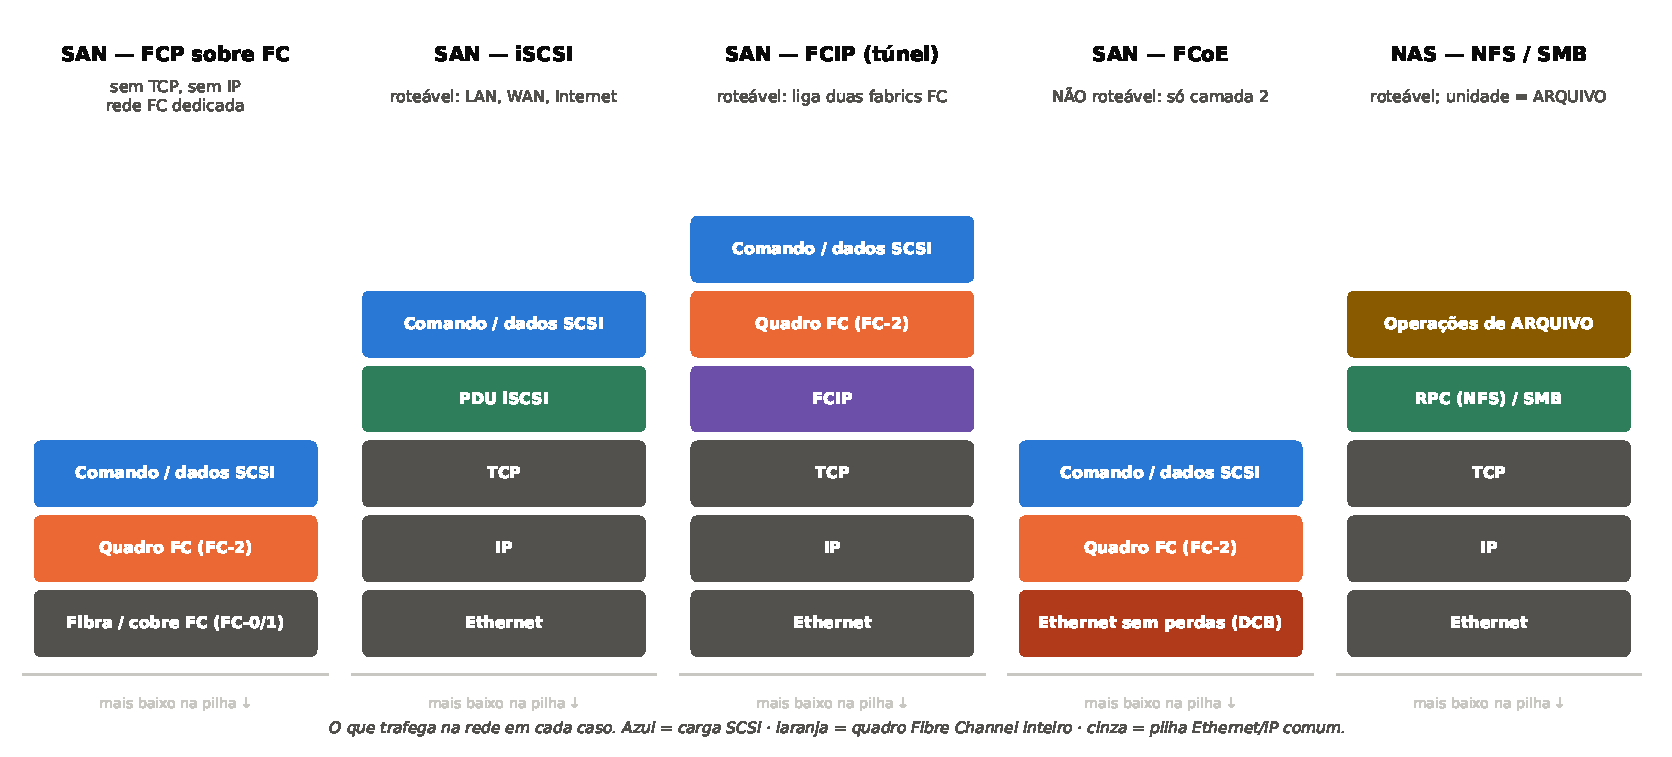
\includegraphics[width=\textwidth]{fig/encapsulamento.pdf}
\caption{O que trafega na rede em cada arquitetura. Três leituras que a figura torna imediatas:
(i) \textbf{iSCSI e FCoE não são variantes um do outro} --- o iSCSI carrega \emph{comandos SCSI}
sobre TCP/IP, enquanto o FCoE carrega o \emph{quadro FC inteiro} sobre Ethernet; (ii) \textbf{FCIP e
FCoE carregam a mesma coisa} (o quadro FC), e diferem apenas em sobre o quê --- daí um ser roteável
e o outro não; (iii) \textbf{o NAS é o único em que a unidade não é o bloco}: no topo da pilha há
operações de arquivo, e não comandos SCSI. Essa última diferença é a da Seção~\ref{sec:nas}, e é a
que decide tudo o mais.}
\label{fig:encaps}
\end{figure}

A Tabela~\ref{tab:protocolos} reúne, em uma única grade, \textbf{todos} os protocolos listados
pelo enunciado, cada um como uma linha, com sua norma de origem e as propriedades que decidem sua
aplicabilidade a um SBD.

\newgeometry{landscape,left=1.4cm,right=1.4cm,top=1.6cm,bottom=1.6cm}
\begin{landscape}\thispagestyle{empty}
{\scriptsize \setlength{\tabcolsep}{3.5pt} \renewcommand{\arraystretch}{1.25}
\begin{longtable}{@{}>{\RaggedRight\arraybackslash}p{1.85cm}
                    >{\RaggedRight\arraybackslash}p{1.15cm}
                    >{\RaggedRight\arraybackslash}p{3.0cm}
                    >{\RaggedRight\arraybackslash}p{2.35cm}
                    >{\RaggedRight\arraybackslash}p{2.75cm}
                    >{\RaggedRight\arraybackslash}p{1.5cm}
                    >{\RaggedRight\arraybackslash}p{2.4cm}
                    >{\RaggedRight\arraybackslash}p{5.5cm}@{}}
\caption{Todos os protocolos exigidos pelo enunciado, com norma de origem e propriedades
decisivas. ``Unidade'' é o que efetivamente trafega na rede.}
\label{tab:protocolos}\\
\toprule
\textbf{Protocolo} & \textbf{Família} & \textbf{Norma / origem} & \textbf{Unidade transportada} &
\textbf{Transporte} & \textbf{Roteável em L3?} & \textbf{Estado em 2026} &
\textbf{Aplicabilidade a SGBD} \\
\midrule
\endfirsthead
\toprule
\textbf{Protocolo} & \textbf{Família} & \textbf{Norma / origem} & \textbf{Unidade transportada} &
\textbf{Transporte} & \textbf{Roteável em L3?} & \textbf{Estado em 2026} &
\textbf{Aplicabilidade a SGBD} \\
\midrule
\endhead
\bottomrule
\endfoot

\textbf{SMB/CIFS} & NAS & Especificação aberta Microsoft [MS-SMB2]; ``CIFS'' $=$ dialeto SMB~1.0
& Operações de arquivo & TCP porta 445 (antes NetBIOS 139) & Sim & SMB~3.1.1 corrente; SMB~1 não
instalado por padrão desde o Windows 10 \textit{Fall Creators Update} \cite{mssmb1} &
\textbf{Suportado} para SQL Server 2012+ (bancos de sistema e de usuário), exigindo SMB~3
\textit{transparent failover} para carga crítica; FILESTREAM não suportado \cite{mssqlsmb} \\

\textbf{NFS} & NAS & IETF: RFC 1094 (v2), RFC 1813 (v3), RFC 7530 (v4.0), \textbf{RFC 8881} (v4.1),
RFC 7862 (v4.2) & Operações de arquivo (RPC) & TCP porta 2049 (v4); v3 usa portmapper $+$ NLM &
Sim & v4.1 é a norma vigente; pNFS separa metadados de dados \cite{rfc8881} & \textbf{Suportado}
com ressalvas: exige \texttt{O\_DIRECT} ou cliente próprio por causa da coerência
\textit{close-to-open} \cite{nfsman}. Oracle implementa cliente próprio (dNFS) \cite{oracledn} \\

\textbf{AFP} & NAS & Proprietário Apple (\textit{AppleTalk Filing Protocol}, 1985--88) & Operações
de arquivo & TCP porta 548 & Sim & \textbf{Encerrado}: servidor removido no macOS 11 (2020);
cliente depreciado no macOS 15.5 (mai./2025) \cite{appleafp}; a Apple informa oficialmente que
destinos AFP do Time Machine deixam de ser suportados no macOS 27 \cite{appleafptm} &
\textbf{Legado, sem recomendação para novas implantações.} Sem travamento em intervalo de \textit{bytes}
adequado; nenhum SGBD de porte o suporta. Migrar para SMB~3 \\

\textbf{FCP sobre FC} & SAN & T11/INCITS (FC-FS, FC-PI); FCP $=$ mapeamento FC-4 de SCSI-3 &
Comandos e dados SCSI em quadros FC & \textit{Fibre Channel} (rede sem perdas por BB\_Credit) &
Não (rede FC própria, endereço de 24 bits) & Padrão do \textit{data center}; 64GFC corrente,
128GFC (Gen 8) em implantação \cite{fcia128} & \textbf{Referência.} Bloco cru, rede dedicada,
latência de rede $<$5\% do acesso NVMe. Base do Oracle ASM e de \textit{clusters} com
armazenamento compartilhado \\

\textbf{FC \textit{Switch}} (\textit{switched fabric}, FC-SW) & SAN & T11/INCITS --- é uma
\textbf{topologia}, não um protocolo & (transporta FCP) & \textit{Fibre Channel} comutado, roteamento
FSPF & Não & Única topologia FC em uso; ponto-a-ponto residual, FC-AL obsoleto &
\textbf{Obrigatória} em produção: banda dedicada por porta, zoneamento, e duas \textit{fabrics}
independentes (SAN A / SAN B) \\

\textbf{iSCSI} & SAN & IETF \textbf{RFC 7143} (2014), que obsoleta a RFC 3720 \cite{rfc7143} &
Comandos SCSI em TCP & TCP porta 3260 sobre Ethernet/IP & \textbf{Sim} --- LAN, WAN e Internet
\cite{elmasri2018} & Consolidado em pequeno e médio porte; acelerado por TOE, iSER e DCB &
\textbf{Muito adequada} quando a rede é dedicada ou segregada. Entrega bloco cru sem o custo de
\textit{fabric} FC \\

\textbf{FCIP} & SAN & IETF \textbf{RFC 3821} (2004) \cite{rfc3821} & \textbf{Quadros FC inteiros}
em TCP/IP & TCP/IP sobre WAN & Sim & Vivo, com propósito único & \textbf{Não é caminho de dado
primário.} É túnel entre duas \textit{fabrics} FC para replicação entre sítios. A distância impõe
latência e normalmente conduz ao modo assíncrono, conforme RPO/RTO (Seção~\ref{sec:fcip}) \\

\textbf{FCoE} & SAN & T11 \textbf{FC-BB-5} $=$ ANSI/INCITS 462-2010; FC-BB-6 (VN2VN)
\cite{fcbb5} & \textbf{Quadros FC inteiros} em quadros Ethernet, \textbf{sem TCP e sem IP} &
Ethernet sem perdas obrigatório: DCB (802.1Qbb PFC, 802.1Qaz ETS, DCBX) $+$ \textit{baby jumbo} &
\textbf{Não} --- ``não é roteável na camada IP e não funcionará através de redes IP roteadas como a
Internet'' \cite{fcbb5} & Nicho: convergência dentro do rack (\textit{blade}, sistemas
convergentes) & \textbf{Viável mas raro.} Perdeu para o iSCSI embaixo e para o FC em cima. Não
atravessa \textit{data centers} \\

\textbf{(fronteira)} \textbf{NVMe-oF} & SAN & NVM Express (FC-NVMe, NVMe/TCP, NVMe/RoCE) & Comandos
NVMe & FC, TCP ou RDMA & Depende do transporte & Em adoção; substitui o \emph{SCSI}, não o meio &
Remove a fila única do SCSI. Fora do escopo dos livros da disciplina; registrado por completude \\

\end{longtable}}
\end{landscape}
\restoregeometry

\subsection{NAS $\times$ SAN: as dimensões que realmente decidem}

\begin{table}[H]
\centering
\caption{Comparação estrutural NAS $\times$ SAN.}
\label{tab:nasxsan}
{\footnotesize
\begin{tabular}{@{}p{3.5cm}p{5.5cm}p{5.5cm}@{}}
\toprule
\textbf{Dimensão} & \textbf{NAS} & \textbf{SAN} \\
\midrule
Unidade de abstração & Arquivo & Bloco (LUN) \\
Dono do sistema de arquivos & O dispositivo de armazenamento & O servidor \\
Rede & LAN Ethernet/IP compartilhada & Rede dedicada (FC) ou Ethernet segregada \\
Protocolos & SMB/CIFS, NFS, AFP & FCP/FC, iSCSI, FCIP, FCoE \\
Compartilhamento entre servidores & Nativo; o dispositivo arbitra & Exige sistema de arquivos de
\textit{cluster} ou LVM ciente de \textit{cluster} \\
Travamento & No protocolo (NLM no NFSv3; integrado a partir do NFSv4; \textit{oplocks}/\textit{leases}
no SMB) & No servidor; a SAN não sabe o que é um arquivo \\
Coerência de \textit{cache} & Fraca por padrão (\textit{close-to-open}) \cite{nfsman} & Não se
aplica: o \textit{cache} é do servidor \\
Custo relativo & Menor (usa infraestrutura existente) & Maior (HBA, \textit{switch}, cabeamento,
pessoal) \\
Distância & Limitada pela LAN & 10 km em fibra \cite{elmasri2018}; ilimitada por FCIP \\
Caso de uso típico em SBD & \textit{Data warehouse}, arquivos de \textit{backup}, ambientes de
desenvolvimento/homologação, bancos de médio porte com dNFS & OLTP crítico, \textit{clusters} com
armazenamento compartilhado, cargas com requisito de latência de \textit{commit} \\
\bottomrule
\end{tabular}}
\end{table}

\destaque{A convergência que os livros já anunciavam}{%
Silberschatz registra: ``sistemas SAN e NAS modernos suportam o uso de uma combinação de discos
magnéticos e SSDs, e podem ser configurados para usar os SSDs como \textit{cache} para dados que
residem em discos magnéticos'' \cite{silberschatz2020}. Na prática de 2026, quase todo
\textit{array} corporativo é \textbf{unificado}: o mesmo equipamento apresenta LUNs por FC ou
iSCSI \emph{e} compartilhamentos por NFS e SMB, sobre o mesmo \textit{pool} de mídia. A pergunta
``comprar NAS ou SAN?'' virou, em grande medida, ``\textbf{qual protocolo apresentar para cada
carga}?'' --- o que é uma pergunta melhor, porque admite respostas diferentes para o
\textit{tablespace} e para a área de \textit{dump}.}

%=====================================================================
\section{AST --- \textit{Automated Storage Tiering}}
\label{sec:ast}
%=====================================================================

\subsection{O que é e por que existe}

Elmasri e Navathe definem: ``outra tendência em armazenamento é o \textit{automated storage
tiering} (AST), que move automaticamente dados entre diferentes tipos de armazenamento, como SATA,
SAS e \textit{solid-state drives} (SSDs), dependendo da necessidade. O administrador de
armazenamento pode configurar uma política de \textit{tiering} na qual dados usados com menos
frequência são movidos para \textit{drives} SATA mais lentos e baratos, e dados usados com mais
frequência são movidos para \textit{solid-state drives}'' \cite{elmasri2018}. E citam a
implementação de referência: ``a EMC tem uma implementação dessa tecnologia chamada FAST (\textit{fully
automated storage tiering}) que faz monitoramento contínuo da atividade de dados e toma ações para
mover os dados para o \textit{tier} apropriado com base na política'' \cite{elmasri2018}.

O AST existe porque a hierarquia de armazenamento de Silberschatz (Seção~\ref{sec:hierarquia}) é
uma \emph{escada de preço por byte}, e a distribuição de acesso a dados é altamente enviesada: em
praticamente qualquer banco de dados corporativo, uma fração pequena dos blocos concentra a
maioria esmagadora dos acessos. Comprar \textit{flash} para o banco inteiro é pagar pelo pior caso
em 100\% da capacidade.

\subsection{Como funciona, concretamente}

Tomamos como exemplo documentado o Dell EMC Unity FAST VP, cujo \textit{white paper} técnico
publica os parâmetros exatos \cite{dellfast}. \textbf{Proveniência:} documentação de fabricante,
produto identificado.

\begin{table}[H]
\centering
\caption{Parâmetros do FAST VP (Dell EMC Unity). Fonte: \textit{white paper} H15086 \cite{dellfast}.}
\label{tab:fast}
{\footnotesize
\begin{tabular}{@{}p{4.2cm}p{10.4cm}@{}}
\toprule
\textbf{Parâmetro} & \textbf{Valor documentado} \\
\midrule
Granularidade de relocação & \textbf{Fatias (\textit{slices}) de 256 MB}: ``em um \textit{pool}
multicamada, os dados dos recursos de armazenamento são espalhados pelos \textit{tiers} pelo FAST
VP em fatias de 256 MB'' \\
\textit{Tiers} definidos & \textit{Extreme Performance} (\textit{flash}); \textit{Performance}
(SAS 10K/15K rpm); \textit{Capacity} (NL-SAS 7,2K rpm) \\
Frequência de análise & ``Uma vez por hora, o FAST VP analisa os dados coletados e classifica cada
fatia com base na \emph{temperatura} de cada fatia'' \\
Janela de relocação & Agendada e configurável; padrão diário, das 17h à 1h \\
Políticas & \textit{Highest Available Tier}; \textit{Auto-Tier}; \textbf{\textit{Start High then
Auto-Tier}} (padrão recomendado); \textit{Lowest Available Tier} \\
\bottomrule
\end{tabular}}
\end{table}

O mecanismo é, portanto: (i) contadores de acesso por fatia; (ii) uma métrica agregada de
``temperatura''; (iii) uma classificação horária; (iv) e a movimentação física das fatias entre
\textit{tiers} durante uma janela em que o impacto sobre a carga de produção é aceitável.

\subsection{A tensão que ninguém menciona: AST versus \textit{buffer pool}}
\label{sec:asttensao}

Aqui está o ponto analítico deste trabalho sobre AST. \textbf{Ressalva de alcance, antes de tudo:}
não afirmamos originalidade absoluta --- as próprias recomendações de fabricante (fixar a política do
volume de \textit{redo}, por exemplo) pressupõem essa tensão sem nomeá-la. O que verificamos é mais
estreito e é o que afirmamos: \textbf{nenhum dos três livros-texto da disciplina faz a ligação entre
a Seção do \textit{buffer manager} e a Seção do \textit{tiering}}, embora ambas estejam no mesmo
capítulo do Elmasri. A contribuição é a \emph{articulação}, não a observação isolada.

\destaque{O SGBD já faz \textit{tiering} --- e faz melhor, mais rápido e com mais informação}{%
Elmasri e Navathe dedicam a Seção 16.3.1 inteira ao \textbf{\textit{buffer manager}}, que ``responde
a requisições por dados e decide qual \textit{buffer} usar e quais páginas substituir'', com
políticas LRU, \textit{clock} e FIFO, além de \textit{pin-count} e \textit{dirty bit}
\cite{elmasri2018}. Isso \emph{é} \textit{tiering} --- entre a memória principal e o armazenamento
secundário. E ele opera com três vantagens decisivas sobre o AST do \textit{array}:

\smallskip
\textbf{(1) Granularidade.} O \textit{buffer manager} decide por \textbf{página de 8 ou 16 KiB}. O
FAST VP decide por \textbf{fatia de 256 MB} \cite{dellfast}. \textbf{Derivação nossa, com a
convenção declarada:} lendo os ``256 MB'' da Dell como 256~MiB,
\[
\frac{256\ \text{MiB}}{16\ \text{KiB}} = \mathbf{16.384\times}
\qquad\text{e}\qquad
\frac{256\ \text{MiB}}{8\ \text{KiB}} = \mathbf{32.768\times}.
\]
\textbf{O fator depende do SGBD}, e por isso publicamos os dois: 16.384$\times$ para a página de
16~KiB do InnoDB e 32.768$\times$ para a de 8~KiB do PostgreSQL e do Oracle. \textbf{Usamos o menor
dos dois em todo o restante do texto}, por ser o mais conservador para o nosso próprio argumento.
(Se os ``256 MB'' forem lidos como decimais, as razões caem para 15.625 e 31.250; adotamos a leitura
binária, usual para tamanhos de bloco.) De todo modo a ordem de grandeza é a mesma: se dentro de uma
fatia houver 1~MB quente e 255~MB frios, o AST promove os 256~MB inteiros.

\smallskip
\textbf{(2) Latência de reação.} O \textit{buffer manager} reage \textbf{ao acesso}. O AST reage em
uma janela de \textbf{horas} \cite{dellfast}.

\smallskip
\textbf{(3) Informação semântica.} O \textit{buffer manager} sabe que aquela página é o nó raiz de
um índice B$^+$-tree e que ela será acessada em toda busca. O \textit{array} vê apenas
\textit{offsets} de LBA.}

Disso decorrem três consequências práticas que devem constar de qualquer recomendação de AST para
SBD:

\begin{enumerate}[leftmargin=0.9cm,itemsep=3pt]
\item \textbf{O AST enxerga a carga \emph{filtrada} pelo \textit{buffer pool}.} O que chega ao
\textit{array} é o \emph{resíduo} que o \textit{cache} do SGBD não absorveu. Um bloco genuinamente
quente pode nunca aparecer como quente para o AST, porque ele mora permanentemente no
\textit{buffer pool} e quase nunca é relido do disco. \textbf{O AST pode, portanto, classificar
como frio exatamente o dado mais quente do banco.}

\item \textbf{Cargas OLTP com dados quentes móveis derrotam o AST.} Se o conjunto quente muda mais
rápido que a janela de relocação (o caso típico de dados particionados por data, em que a partição
quente muda diariamente), o AST passa a maior parte do tempo movendo dados que acabaram de esfriar.
A política \textit{Start High then Auto-Tier}, que a Dell recomenda como padrão \cite{dellfast},
existe precisamente para mitigar isso: escreve tudo no \textit{tier} mais rápido primeiro e só
depois esfria o que não for acessado.

\item \textbf{\textit{Caching} é mais adequado que \textit{tiering} para banco de dados.} A
distinção é importante e frequentemente confundida: no \textit{tiering}, o dado \emph{muda de
lugar} (só existe uma cópia, num \textit{tier}); no \textit{caching}, o dado é \emph{copiado} para
a camada rápida e o original permanece. \textit{Caching} reage em segundos e com granularidade
fina, sem custo de migração; \textit{tiering} reage em horas com granularidade grossa, mas
converte capacidade cara em capacidade barata de forma permanente. Para OLTP, \textit{caching} é
quase sempre a resposta certa. Não por acaso, Silberschatz descreve exatamente essa configuração:
``sistemas SAN e NAS modernos [...] podem ser configurados para usar os SSDs como \textbf{cache}
para dados que residem em discos magnéticos'' \cite{silberschatz2020}.
\end{enumerate}

\subsection{Recomendação sobre AST}

\begin{itemize}[leftmargin=0.7cm,itemsep=2pt]
\item \textbf{Habilitar} em \textit{data warehouses} e ambientes com particionamento por data e
grande volume histórico frio: o padrão de acesso é estável em escala de dias, que é a escala do
AST.
\item \textbf{Habilitar} em consolidação de muitos bancos pequenos num \textit{pool} comum, em que
o desbalanceamento de temperatura entre bancos é grande e persistente.
\item \textbf{Evitar} (ou fixar em \textit{Highest Available Tier}) para arquivos de
\textit{redo}/WAL, \textit{tempdb} e índices críticos: são estruturas cujo desempenho não pode
depender de uma decisão estatística tomada com atraso de horas.
\item \textbf{Nunca} usar AST como substituto de dimensionamento. Se o conjunto de dados quente não
cabe no \textit{tier} rápido, o AST não cria capacidade --- ele apenas redistribui a escassez, e
acrescenta tráfego de migração à carga já saturada.
\end{itemize}

\subsection{AST, cache, ILM, HSM, backup e replicação}

\begin{center}\footnotesize
\begin{tabular}{@{}p{2.2cm}p{3.1cm}p{3.2cm}p{3.2cm}p{3.3cm}@{}}
\toprule
\textbf{Mecanismo} & \textbf{Objetivo/gatilho} & \textbf{O dado muda ou é copiado?} &
\textbf{Recuperação} & \textbf{Não substitui} \\
\midrule
Cache & Reduzir latência; acesso recente/frequente & Cópia rápida; original permanece &
Não é cópia de recuperação & Backup, replicação, capacidade \\
AST/tiering & Ajustar custo/desempenho; telemetria por faixa & Em geral muda de tier &
Depende do array; não cria histórico & Backup e dimensionamento \\
ILM & Aplicar política ao ciclo de vida, retenção e classe & Move/copia conforme política &
Pode incluir retenção, mas exige desenho & Backup testado e governança \\
HSM & Migrar arquivos frios preservando um stub & Move para mídia secundária/terciária &
Reidratação sob demanda & Backup independente \\
Backup & Recuperar estado anterior por RPO/RTO & Cria cópia versionada e independente &
Restauração testada & Alta disponibilidade \\
Replicação & Disponibilidade/DR; síncrona ou assíncrona & Cria réplica do estado corrente &
Failover; corrupção lógica pode propagar & Histórico de backup \\
\bottomrule
\end{tabular}
\end{center}

\noindent A decisão deve registrar \textbf{RPO}, \textbf{RTO}, domínio de falha, retenção e
resultado de teste de restauração/failover. AST otimiza posicionamento; não cria, por si só,
uma cópia recuperável.

%=====================================================================
\section{\textit{Object-Based Storage}}
\label{sec:objeto}
%=====================================================================

\subsection{O terceiro paradigma}

Bloco e arquivo não são as duas únicas abstrações possíveis. Elmasri e Navathe apresentam a
terceira: ``sob esse esquema, os dados são gerenciados na forma de \textbf{objetos}, em vez de
arquivos feitos de blocos. Os objetos carregam \textbf{metadados} que contêm propriedades que podem
ser usadas para gerenciá-los. Cada objeto carrega um \textbf{identificador global único} que é
usado para localizá-lo'' \cite{elmasri2018}.

\begin{table}[H]
\centering
\caption{Os três paradigmas de armazenamento em rede.}
\label{tab:paradigmas}
{\footnotesize
\begin{tabular}{@{}p{2.5cm}p{3.5cm}p{3.5cm}p{4.4cm}@{}}
\toprule
& \textbf{Bloco (SAN)} & \textbf{Arquivo (NAS)} & \textbf{Objeto} \\
\midrule
Unidade & Bloco de tamanho fixo & Arquivo em hierarquia de diretórios & Objeto com metadados e ID
global \\
Endereçamento & LUN $+$ LBA & Caminho hierárquico & Espaço de nomes plano (\textit{bucket} $+$
chave) \\
Interface & SCSI / NVMe & POSIX, SMB, NFS & HTTP REST (\textsc{put}, \textsc{get},
\textsc{delete}) \\
Atualização parcial & Sim, qualquer bloco & Sim, qualquer \textit{offset} & Em APIs S3,
\textsc{put} substitui o valor da chave; multipart não é atualização in-place \\
Escala típica & Terabytes a petabytes & Terabytes a petabytes & \textbf{Exabytes} \\
Metadados & Nenhum (o \textit{array} não sabe o que guarda) & Fixos (dono, datas, permissões) &
\textbf{Arbitrários, definidos pela aplicação} \\
Consistência/locking & Definidos pelo host/SGBD & NFS/SMB oferecem locks/leases conforme versão &
S3 é forte por chave/listagem; não há transação/lock entre chaves \cite{awss3consistency} \\
Disponibilidade & Depende de duas fabrics, MPIO e array & Depende de nós/cluster e failover do
protocolo & Distribuída pelo serviço; conferir SLA e região \\
Melhor uso & OLTP, logs, clusters homologados & Compartilhamento, DW, dumps e SGBD homologado &
Data lake, backup, arquivo e dados não estruturados \\
Limitação principal & Custo/operação e compartilhamento exige coordenação & Semântica e latência
dependem do protocolo/cliente & Latência de API e ausência de atualização/ordenação entre chaves \\
Exemplos & LUN FC/iSCSI/NVMe-oF & NFSv4.1, SMB 3 & Amazon S3, Ceph RGW, MinIO \\
\bottomrule
\end{tabular}}
\end{table}

\subsection{Origem acadêmica}

Elmasri e Navathe registram a genealogia corretamente: ``o armazenamento por objetos tem suas
origens em projetos de pesquisa na CMU (Gibson et al., 1996) sobre escalabilidade de
\textit{network attached storage} e no sistema \textit{OceanStore} em UC Berkeley (Kubiatowicz et
al., 2000), que tentava construir uma infraestrutura global sobre todas as formas de servidores
confiáveis e não confiáveis para acesso contínuo a dados persistentes'' \cite{elmasri2018}.
Registram também a tentativa de padronização: ``comandos de dispositivo de armazenamento baseado em
objeto (OSDs) foram propostos como parte do protocolo SCSI há muito tempo, mas não se tornaram
produto comercial até que a Seagate adotou OSDs em sua plataforma \textit{Kinetic Open Storage}''
\cite{elmasri2018}.

\destaque{A mesma ideia arquitetural aparece três vezes neste trabalho, com nomes diferentes}{%
O que o NASD de Gibson \textit{et al.} propôs em 1996 não foi ``guardar objetos''. Foi
\textbf{separar o caminho de metadados e autorização do caminho de dados}: o cliente pede ao
servidor de metadados uma \emph{capacidade} (um \textit{token} criptográfico que autoriza um acesso
específico) e depois fala \emph{direto} com o dispositivo de armazenamento, sem que os dados passem
pelo servidor. O gargalo deixa de ser o servidor de arquivos.

\smallskip
\textbf{É exatamente a mesma ideia de:}
\begin{itemize}[leftmargin=0.7cm,itemsep=1pt,topsep=2pt]
\item \textbf{pNFS} (NFSv4.1, Seção~\ref{sec:nfs}): o cliente obtém um \textit{layout} do servidor de
      metadados e lê os dados diretamente dos servidores de dados \cite{rfc8881};
\item \textbf{NDMP} (Seção~\ref{sec:recterciario}): o servidor de \textit{backup} controla, mas os
      dados vão do NAS direto para a fita;
\item \textbf{Amazon Aurora} (Seção~\ref{sec:recsecundario}): o motor manda \textit{log} e a camada
      de armazenamento materializa as páginas por conta própria \cite{aurora2017}.
\end{itemize}

\textbf{A observação que tiramos disso:} a ``terceira via'' do armazenamento não é o objeto ---
é a \emph{desagregação do plano de controle e do plano de dados}. O objeto é uma das formas que ela
assumiu; o pNFS é outra, dentro do NAS; o Aurora é outra, dentro do SGBD. Ler os três como
instâncias do mesmo movimento explica por que o objeto venceu onde venceu e por que não venceu em
OLTP: o que ele desagrega bem é a leitura em massa, não a ordenação de escrita.}

\correcao{Nota de atualização sobre a Seagate Kinetic}{%
O exemplo da Seagate Kinetic era corrente na edição de 2016 do livro. A plataforma
\textbf{não obteve tração comercial}: a cobertura técnica de março de 2016 registra que a HGST
``passou um ano tentando encontrar casos de uso que valessem a pena para \textit{drives} Kinetic
junto a seus clientes, e não achou nenhum'', e que o projeto poderia voltar a ser apenas uma
iniciativa proprietária da Seagate \cite{theregister2016}.
Na mesma linha, a padronização OSD no T10 não se estabeleceu como caminho da indústria.

\smallskip
\textbf{Declaração de lacuna:} \emph{não localizamos} anúncio formal de descontinuação da plataforma
Kinetic. Dizer ``foi descontinuada'' seria afirmar mais do que a fonte sustenta; dizemos ``não
obteve tração comercial'', que é o que está documentado.

\smallskip
\textbf{O que venceu foi outro caminho --- e é justo dizer que o próprio livro já aponta para ele.}
Elmasri e Navathe escrevem, no mesmo trecho, que ``o armazenamento por objetos é a escolha de muitas
ofertas de nuvem, como o S3 da AWS e o Azure da Microsoft'', e que ``o OpenStack Swift é um projeto
de código aberto que permite usar HTTP \textsc{get} e \textsc{put} para recuperar e armazenar
objetos --- essa é basicamente toda a API'' \cite{elmasri2018}. \textbf{Não há, portanto, novidade
nossa em dizer que o verbo HTTP venceu o comando SCSI: o livro registra o fato.} O que
acrescentamos é apenas a consequência de dez anos depois --- que a API do S3 especificamente virou
a interface que os demais implementam por compatibilidade (Ceph RADOS Gateway, MinIO,
\textit{appliances} corporativos). \textbf{Categoria:} leitura de mercado nossa, apoiada na
ubiquidade das implementações, \emph{sem} fonte primária que a quantifique --- e portanto
apresentada como leitura, não como fato.}

\subsection{Propriedades: por que escala tanto}

O armazenamento por objetos abre mão de coisas para ganhar escala. Cada renúncia é deliberada:

\begin{itemize}[leftmargin=0.7cm,itemsep=3pt]
\item \textbf{Abre mão da hierarquia} $\rightarrow$ o espaço de nomes plano é particionável por
\textit{hash} sem coordenação central, o que remove o gargalo do servidor de metadados.
\item \textbf{Abre mão da atualização parcial} $\rightarrow$ objetos imutáveis eliminam
\textit{read-modify-write} distribuído, tornam a replicação trivialmente correta e permitem
versionamento nativo.
\item \textbf{Abre mão do POSIX} $\rightarrow$ sem \texttt{fsync}, sem travamento em intervalo de
\textit{bytes}, sem semântica de \textit{rename} atômico; sobra HTTP, que atravessa qualquer rede.
\item \textbf{Em troca, ganha durabilidade extrema por codificação de apagamento.} A AWS declara
que o S3 é ``projetado para durabilidade de \textbf{99,999999999\% (11 noves)}''
\cite{awss3faq}. Trata-se de \textbf{objetivo de projeto}, não de SLA nem de probabilidade
empírica independente por objeto. Portanto, não o convertemos em anos até uma perda:
essa extrapolação ocultaria falhas correlacionadas, exclusão por credencial válida,
corrupção lógica e \textit{ransomware}.
\end{itemize}

\destaque{Uma atualização essencial: o S3 não é mais eventualmente consistente}{%
Durante 14 anos, a objeção padrão ao armazenamento por objetos para dados de banco era a
\textbf{consistência eventual}: após uma escrita, uma leitura podia devolver a versão antiga. Isso
mudou. Desde \textbf{dezembro de 2020}, a AWS documenta que o S3 fornece ``consistência forte
\textit{read-after-write} automaticamente'', de modo que, ``após uma escrita ou sobrescrita bem
sucedida, requisições de leitura subsequentes recebem imediatamente a versão mais recente do
objeto'', valendo também para operações de listagem \cite{awss3faq}. \textbf{Qualquer texto que
ainda afirme que o S3 é eventualmente consistente está desatualizado em mais de cinco anos} --- e
essa era uma das afirmações que a nossa própria primeira versão continha (ver
Seção~\ref{sec:erros}).}

\subsection{Por que ainda não serve como armazenamento primário de OLTP}

Elmasri e Navathe encerram a seção com uma ressalva que continua correta: ``como o armazenamento
por objetos força o travamento a ocorrer no nível do objeto, não está claro quão adequado ele é
para processamento concorrente de transações em sistemas orientados a transações de alta vazão.
Portanto, ainda não é considerado viável para aplicações de banco de dados corporativas de
\textit{mainstream}'' \cite{elmasri2018}. Detalhando as razões contra os cinco requisitos da
Seção~\ref{sec:engine}:

\begin{enumerate}[leftmargin=0.9cm,itemsep=2pt]
\item \textbf{Sem atualização in-place no modelo S3.} Alterar uma linha exige publicar novo valor
para a chave; multipart upload muda o transporte, não a semântica de substituição. Um
\textit{tablespace} de 100 GB como um objeto é inviável; fatiado em objetos de 8 KiB, perde-se toda
a vantagem de escala e ganha-se uma requisição HTTP por página.
\item \textbf{Latência de uma ordem de grandeza acima.} Silberschatz já registrava:
``armazenamento em nuvem tem latência muito alta, de dezenas a centenas de milissegundos, se os
dados não estiverem colocalizados com o banco de dados, e portanto não é ideal como armazenamento
subjacente para bancos de dados'' \cite{silberschatz2020}.
\item \textbf{Sem \texttt{fsync} nem ordenação de escrita} entre objetos distintos: não há como
exprimir ``grave o \textit{log} antes da página''.
\item \textbf{Granularidade de travamento incompatível} com concorrência transacional.
\end{enumerate}

\subsection{Onde ele venceu, e venceu completamente}

\begin{itemize}[leftmargin=0.7cm,itemsep=2pt]
\item \textbf{Camada de armazenamento de \textit{data warehouses} em nuvem.} A arquitetura de
separação entre computação e armazenamento (Snowflake, Databricks, BigQuery) coloca os dados em
objetos imutáveis em formato colunar (Parquet, ORC), com uma camada de metadados transacional por
cima (Iceberg, Delta Lake). O padrão de acesso --- escrever uma vez, ler muitas, varrer grandes
extensões --- é exatamente aquele em que o objeto é ótimo e a latência não importa.
\item \textbf{Destino de \textit{backup} e arquivamento} (Seção~\ref{sec:recterciario}).
\item \textbf{Repositórios de dados não estruturados.} Elmasri e Navathe citam Facebook, Spotify e
Dropbox \cite{elmasri2018}; o caso do Dropbox é discutido na Seção~\ref{sec:exemplos}.
\end{itemize}

%=====================================================================
\section{Recomendação geral}
\label{sec:recomendacao}
%=====================================================================

Esta seção responde à pergunta central do enunciado: \emph{quando optar por um ou pelo outro tipo
de \textit{storage}, considerando como o núcleo do SBD (\textit{Database Engine}) utilizará a
solução, tanto em nível secundário (\textit{online}) quanto em nível terciário (\textit{offline})}.

\subsection{Princípio orientador}

\destaque{A regra de decisão, em uma frase}{%
\textbf{Escolha pela semântica oficialmente suportada pelo SGBD e pelo SLA, não apenas pela
velocidade do enlace.} Bloco/SAN é frequente em OLTP e \textit{clusters} compartilhados,
mas NFS/SMB homologados (como dNFS e SMB 3) também podem fornecer durabilidade, locking e
failover adequados. Compare protocolo/cliente, latência de cauda, disponibilidade, RPO/RTO,
benchmark e TCO; não se presume equivalência nem menor custo sem medir a configuração.
Objeto é indicado quando a aplicação foi projetada para sua API e sua granularidade.}

O cálculo da Seção~\ref{sec:topologias} mostra somente que \textbf{dois saltos de comutação
local FC}, nas condições do datasheet, somam menos de 5\% de um acesso NVMe de 20\,$\mu$s.
Ele exclui HBA, serialização, cabos, ISLs, filas, controladora e alvo; portanto não prova
que a rede fim a fim deixou de ser gargalo. O resultado serve para isolar o custo do
switch, enquanto a decisão completa continua dependendo de semântica e medições.

\subsection{Nível secundário (\textit{storage online})}
\label{sec:recsecundario}

É onde vivem os arquivos de dados, os índices e o \textit{log} de transações --- tudo que o motor
acessa durante a execução normal. A recomendação é por \textbf{tipo de carga}, não por tipo de
empresa.

\begin{table}[H]
\centering
\caption{Recomendação para o nível secundário, por perfil de carga.}
\label{tab:recsec}
{\footnotesize
\begin{tabular}{@{}p{3.5cm}p{2.6cm}p{8.4cm}@{}}
\toprule
\textbf{Perfil de carga} & \textbf{Recomendação} & \textbf{Justificativa} \\
\midrule
OLTP crítico, alta taxa de \textit{commit} & \textbf{SAN ou NAS homologado e medido} &
A latência de \texttt{fsync} do \textit{log} governa a vazão. Bloco oferece controle direto;
NFS/SMB só entra com suporte oficial, persistência/locking corretos, failover e benchmark de cauda. \\
\addlinespace
\textit{Cluster} com armazenamento compartilhado (Oracle RAC) & \textbf{SAN} (bloco) &
Vários nós escrevem nos mesmos blocos com coordenação própria do SGBD (Oracle ASM sobre LUNs). É a
configuração de referência do fornecedor. \\
\addlinespace
Banco relacional de médio porte, OLTP moderado & \textbf{NAS ou SAN, após validação} &
NFSv4.1 com \texttt{O\_DIRECT}/dNFS \cite{oracledn} pode ser adequado, mas a escolha exige
matriz de suporte, teste de falha, latência P99 e TCO da configuração completa. \\
\addlinespace
\textit{Data warehouse}, OLAP, varredura sequencial & \textbf{NAS ou objeto} & Acesso em
extensões grandes reduz a sensibilidade à latência por operação; medir banda, concorrência,
custo por TB/TCO e compatibilidade do motor antes de escolher. \\
\addlinespace
Desenvolvimento, homologação, muitas instâncias pequenas & \textbf{NAS} & Provisionamento simples,
\textit{clones} finos por instantâneo de arquivo, e nenhum requisito de latência. \\
\addlinespace
Área de \textit{dump}, \textit{export}, \textit{staging} de ETL & \textbf{NAS} & Semântica de
arquivo é exatamente a abstração desejada; e escrever \textit{dumps} num LUN dedicado é
desperdício. \\
\addlinespace
Banco em nuvem gerenciado & \textbf{Bloco de rede} (equivalente a SAN) & Volumes de bloco em nuvem
(EBS e equivalentes) são SAN sob outro nome: iniciador no \textit{host}, alvo remoto, semântica de
bloco. \\
\bottomrule
\end{tabular}}
\end{table}

\destaque{A observação que mais surpreende: o modelo pode ser abandonado por inteiro}{%
Há um terceiro caminho, que não é NAS nem SAN, e que a arquitetura do \textbf{Amazon Aurora}
exemplifica. Em vez de escolher entre bloco e arquivo, ela \textbf{redesenha a fronteira}: ``as
únicas escritas que cruzam a rede são registros de \textit{redo log}. Nenhuma página é jamais
escrita a partir da camada de banco de dados'', porque ``o \textit{log} é o banco de dados, e
quaisquer páginas que o sistema de armazenamento materialize são simplesmente um \textit{cache}''
\cite{aurora2017}. Os autores justificam a decisão exatamente com o argumento desta seção: ``o
gargalo se move para a rede entre a camada de banco de dados que requisita E/S e a camada de
armazenamento'' \cite{aurora2017}.

\smallskip
\textbf{Resultado publicado.} No experimento da Tabela 1 do artigo (SIGMOD 2017), o Aurora sustentou
\textbf{27.378.000} transações contra \textbf{780.000} do MySQL espelhado sobre EBS --- ``35 vezes
mais transações'' --- com \textbf{0,95} operações de E/S por transação contra \textbf{7,4}, que o
artigo descreve como ``7,7 vezes menos'' \cite{aurora2017}. \textbf{Proveniência:} medição publicada
em artigo revisado por pares; os números são do experimento específico descrito no artigo e não
devem ser generalizados como desempenho de produto.

\smallskip
\textbf{Divergência que encontramos ao conferir a conta:} $7{,}4 \div 0{,}95 = 7{,}79$, isto é,
\textbf{7,8}$\times$ e não os 7,7$\times$ que o texto do artigo enuncia. A diferença é de
arredondamento e irrelevante para o argumento, mas registramos porque a regra deste trabalho é
refazer toda conta citada --- inclusive as de artigos revisados por pares.

\smallskip
\textbf{Por que isso importa para a pergunta do enunciado:} a resposta ``NAS ou SAN?'' pressupõe que
o motor escreva páginas. Quando o motor deixa de escrever páginas e passa a escrever só
\textit{log}, a pergunta muda de objeto.}

\subsection{Nível terciário (\textit{storage offline})}
\label{sec:recterciario}

\destaque{Antes de comparar mídias: a pergunta que o enunciado faz é NAS $\times$ SAN}{%
A Seção~\ref{sec:hierarquia} estabeleceu que NAS e SAN são, ambos, tecnologias de nível
\emph{secundário}. Isso poderia sugerir que a pergunta ``NAS ou SAN?'' não se aplica ao nível
terciário. \textbf{Aplica-se, e de três maneiras concretas:}

\smallskip
\textbf{(1) A biblioteca de fitas é um dispositivo de SAN.} A especificação do LTO-10 declara sua
taxa comprimida ``usando a interface \textit{Fibre Channel} de 32 Gb'' \cite{lto10}. Os
\textit{drives} de fita são alvos FC (ou SAS) na mesma \textit{fabric} dos \textit{arrays}. A
consequência de projeto é direta: \textbf{a janela de \textit{backup} disputa a mesma
\textit{fabric} que a carga de produção}, e o zoneamento precisa separá-las. Um \textit{backup}
completo a 400 MB/s por \textit{drive}, com oito \textit{drives} em paralelo, são 3,2 GB/s
sustentados atravessando a SAN --- comparável à carga OLTP de pico de muitas instalações.

\smallskip
\textbf{(2) O estágio intermediário é NAS.} A prática dominante não escreve do banco direto para a
fita: escreve primeiro em disco (\textit{disk-to-disk-to-tape}), e esse estágio é quase sempre um
compartilhamento NAS --- semântica de arquivo é exatamente a abstração desejada para um conjunto de
arquivos de \textit{dump} nomeados por data. O NAS é, portanto, a \textbf{porta de entrada} do nível
terciário.

\smallskip
\textbf{(3) Fazer \textit{backup} de um NAS exige um protocolo próprio: o NDMP.} Um NAS
corporativo não roda agente de \textit{backup}; o \textbf{NDMP} (\textit{Network Data Management
Protocol}) separa o canal de \emph{controle} (o servidor de \textit{backup} orquestra) do canal de
\emph{dados} (o NAS escreve direto no \textit{drive} de fita, sem que os dados atravessem o servidor
de \textit{backup}). É o análogo, no mundo de arquivo, da separação metadados/dados do pNFS e do
NASD --- e é o elo que liga NAS, SAN e nível terciário numa única arquitetura.
\textbf{Declaração de escopo:} não aprofundamos o NDMP porque o enunciado não o lista; registramos
por ser a resposta correta à pergunta ``como se faz \textit{backup} de um NAS?''.}

\smallskip
Estabelecido o papel de cada arquitetura, resta a escolha de mídia. Silberschatz define o nível
terciário como o de ``fita magnética e \textit{jukeboxes} de disco óptico'' \cite{silberschatz2020}. Elmasri e Navathe: ``discos ópticos e fitas são mídias removíveis
usadas nos sistemas de hoje como armazenamento \textit{offline} para arquivamento de bancos de
dados'' \cite{elmasri2018}. As duas opções realistas em 2026 são \textbf{fita} e
\textbf{armazenamento por objetos em classe de arquivamento}.

\subsubsection*{Fita: viva, e ligada à SAN}

O LTO Program publica para a geração 10, lançada em 2025: cartuchos de ``\textbf{30 TB e 40 TB de
capacidade nativa}'', atingindo ``75 TB e 100 TB respectivamente com razão de compressão de
2,5:1'', e ``velocidades máximas de transferência de \textbf{400 MB/s (nativa)} e 1.200 MB/s
(comprimida a 2,5:1, usando a interface \textit{Fibre Channel} de 32 Gb)'' \cite{lto10}.
\textbf{Proveniência:} especificação do consórcio LTO.

\correcao{Atualizando o Elmasri \& Navathe sobre fita}{%
O livro registra o estado da tecnologia de fita em 2016: ``o consórcio LTO [\ldots] lançou o padrão
LTO-6 mais recente em 2012 [\ldots] A geração atual de bibliotecas usa \textit{drives} LTO-6, com
cartucho de 2,5 TB e taxa de transferência de 160 MB/s'' \cite{elmasri2018}. Confrontando com a
especificação vigente \cite{lto10}:
\[
\text{capacidade: } \frac{40\ \text{TB}}{2{,}5\ \text{TB}} = \mathbf{16\times}
\qquad
\text{taxa: } \frac{400\ \text{MB/s}}{160\ \text{MB/s}} = \mathbf{2{,}5\times}
\]
\textbf{Consequência prática, e ela é contraintuitiva:} em dez anos a capacidade cresceu $16\times$
e a taxa apenas $2{,}5\times$. \textbf{O tempo para ler um cartucho cheio, portanto, aumentou
${\approx}6{,}4\times$} --- de $2{,}5\times10^{12} \div 160\times10^{6} = 4{,}3$~h no LTO-6 para
27,8~h no LTO-10 (Seção~\ref{sec:recterciario}). A fita ficou muito mais densa e proporcionalmente
muito mais lenta de esvaziar, o que desloca a decisão de arquivamento do custo por TB para o
\textbf{tempo de recuperação}. \textbf{Categoria:} atualização de dado datado, com derivação nossa
da consequência.}

\correcao{Rótulo obrigatório: nativo $\neq$ comprimido}{%
A indústria de fita publica \emph{sempre} os dois números, e a diferença é de $2{,}5\times$ ---
assumida, não medida. \textbf{Dados de banco de dados já comprimidos pelo próprio SGBD não atingem
2,5:1}, e frequentemente não passam de 1,2:1. Dimensionar uma biblioteca de fitas pela capacidade
comprimida de catálogo é o erro mais comum do planejamento de \textit{backup}. Neste relatório,
sempre que citamos capacidade de fita, o número nativo é o número.}

\correcao{Achado da nossa verificação por script: a especificação do LTO não fecha}{%
A regra do grupo de \emph{refazer toda conta citada} pegou uma inconsistência na fonte primária.
O LTO Program publica, para a mesma geração 10 \cite{lto10}:
\begin{itemize}[leftmargin=0.7cm,itemsep=1pt,topsep=2pt]
\item capacidade: 30 e 40 TB nativos, ``75 TB e 100 TB respectivamente com razão de compressão de
      2,5:1'' --- \textbf{fecha}: $30 \times 2{,}5 = 75$ e $40 \times 2{,}5 = 100$;
\item taxa: ``400 MB/s (nativa) e 1.200 MB/s (comprimida a \textbf{2,5:1})'' --- \textbf{não fecha}:
      $400 \times 2{,}5 = \mathbf{1.000}$, e não 1.200. Os 1.200 implicariam razão de \textbf{3:1}.
\end{itemize}
\textbf{Não sabemos qual dos dois números a fonte pretendia}, e não o adivinhamos. Registramos a
inconsistência e adotamos, em todo este relatório, \textbf{apenas a taxa nativa de 400 MB/s} --- que
é a única não derivada de uma razão de compressão assumida, e a única que se aplica a dados de banco
já comprimidos pelo SGBD. \textbf{Categoria: divergência na fonte primária, declarada.}}

Note-se ainda o detalhe revelador na especificação: a taxa comprimida é declarada
\emph{``usando a interface \textit{Fibre Channel} de 32 Gb''} \cite{lto10}. Ou seja: a biblioteca de
fitas moderna é um \textbf{dispositivo da SAN}. O nível terciário não é um mundo à parte --- ele é
conectado pela mesma \textit{fabric} do nível secundário, e o dimensionamento do enlace FC precisa
contemplar a janela de \textit{backup}.

\subsubsection*{Objeto em classe de arquivamento}

A alternativa é o armazenamento por objetos em classe fria. A AWS publica, para o S3 Glacier Deep
Archive, preço de ``\textbf{US\$ 0,00099 por GB-mês (ou US\$ 1 por TB-mês)}'' e prazos de
recuperação ``de \textbf{12 a 48 horas}'' \cite{awsglacier}. \textbf{Proveniência:} preço de tabela
do fabricante, \textbf{consultado em setembro de 2026}; preço de nuvem é número volátil e não deve
ser reproduzido sem data.

Os prazos de recuperação são justamente o que faz dessa classe um armazenamento \emph{terciário} na
definição de Silberschatz: ela não é acessível sem uma operação de restauração explícita, do mesmo
modo que uma fita precisa ser montada. Para comparação, o mesmo documento da AWS registra
recuperação em ``milissegundos'' para o \textit{Glacier Instant Retrieval} e ``tipicamente 3 a 5
horas'' para a recuperação padrão do \textit{Glacier Flexible Retrieval} \cite{awsglacier}.

\begin{table}[H]
\centering
\caption{Recomendação para o nível terciário.}
\label{tab:recter}
{\footnotesize
\begin{tabular}{@{}p{4.2cm}p{4.9cm}p{5.4cm}@{}}
\toprule
\textbf{Critério} & \textbf{Fita (LTO em biblioteca)} & \textbf{Objeto em classe de arquivamento} \\
\midrule
Custo por TB armazenado & Menor no longo prazo; capital inicial alto (a biblioteca) & US\$ 1 por
TB-mês no Deep Archive (set./2026) \cite{awsglacier}; sem capital inicial \\
Custo de recuperação & Baixo e previsível (tempo de operador e de \textit{drive}) &
\textbf{Cobrado por volume recuperado} --- é o custo que quebra orçamentos de restauração em massa \\
Prazo de recuperação & Minutos a horas (montagem $+$ posicionamento sequencial) & 12 a 48 h no Deep
Archive \cite{awsglacier} \\
Isolamento contra \textit{ransomware} & \textbf{Vantagem decisiva}: o cartucho fora do \textit{drive}
é um \textit{air gap} físico, inatingível por rede & Depende de \textit{object lock} / WORM
configurado corretamente; a proteção é lógica, não física \\
Longevidade e migração & Compatibilidade de leitura limitada a poucas gerações; exige migração
periódica & Migração é responsabilidade do provedor \\
Recomendação & Arquivo legal de longo prazo, cópia final da regra 3-2-1, volumes muito grandes &
Retenção operacional, conformidade com recuperação rara, quando não se quer operar
\textit{hardware} \\
\bottomrule
\end{tabular}}
\end{table}

\destaque{A recomendação prática para o nível terciário}{%
\textbf{Não escolha: combine.} A prática consolidada é a regra \textbf{3-2-1} --- três cópias, em
dois tipos de mídia, uma delas fora do sítio. Um desenho defensável para um SBD corporativo:
(i) \textit{backup} operacional em disco no NAS, para restauração rápida dos últimos dias;
(ii) cópia em objeto, classe de arquivamento, para retenção de meses a anos; (iii) cópia em fita
com cartucho ejetado, para arquivo de longo prazo e forte isolamento físico. A fita não é o
único mecanismo defensivo: contas/vaults isolados, imutabilidade e cópias offline também
reduzem o alcance de credenciais comprometidas. Cada cópia deve ter restauração testada,
RPO, RTO e domínio de falha explícitos.}

%=====================================================================
\section{Exemplos reais}
\label{sec:exemplos}
%=====================================================================

\destaque{Critério de seleção}{%
O enunciado pede ``exemplos reais, tais como aquele mostrado em sala de aula usando um vídeo do
YouTube''. Não tivemos acesso ao vídeo específico exibido em aula. Em vez de supor qual era,
adotamos um critério explícito: \textbf{só entram exemplos com documentação primária verificável}
--- artigo revisado por pares, documentação técnica do próprio operador, ou especificação de
fabricante. Casos citados apenas em material de divulgação foram descartados.}

\subsubsection*{(1) CERN --- escala de exabyte com objeto, disco e fita}

O CERN publica que o seu \textit{data centre} ``costumava \textbf{processar}, em média, um petabyte
(um milhão de \textit{gigabytes}) de dados por dia durante o LHC Run 2'', e que o plano para o Run 3
era armazenar ``mais de 600 petabytes de dados'', com as instâncias do sistema EOS excedendo ``sete
bilhões de arquivos (em junho de 2022)'' \cite{cernstorage}. \textbf{Proveniência:} documentação do
próprio operador; \textbf{data carimbada: junho de 2022}.

\correcao{Rótulo: ``processar'' não é ``gravar''}{%
A nossa primeira versão escreveu que o CERN ``gravou 1 PB por dia''. O texto do CERN diz
\emph{process} \cite{cernstorage}, e processar inclui o que é filtrado e descartado pelos sistemas
de \textit{trigger} --- que descartam a esmagadora maioria dos eventos. A correção foi apontada pela
rodada de verificação adversarial e é exatamente o tipo de erro que este relatório classifica como
``número certo descrevendo outra coisa''.}

A arquitetura combina os três paradigmas: EOS como camada de disco distribuída, CTA (\textit{CERN
Tape Archive}) como camada de fita, e Ceph para armazenamento de bloco e objeto da infraestrutura de
nuvem interna \cite{cerncta}. É a demonstração mais clara de que, em escala extrema, a pergunta deixa
de ser ``NAS ou SAN'' e passa a ser ``qual camada para qual etapa do ciclo de vida do dado''.

\subsubsection*{(2) Dropbox --- a migração de volta para infraestrutura própria}

O Dropbox operou por anos sobre o Amazon S3 e migrou aproximadamente \textbf{500 petabytes} de
dados de usuário para o seu próprio sistema de armazenamento por objetos, o \textbf{Magic Pocket}.
\textbf{Precisão de rótulo:} a publicação do próprio Dropbox, de julho de 2016, declara que ``agora
servimos \textbf{90\%} dos dados de nossos clientes no Magic Pocket'' \cite{dropboxmp} --- 90\%, não
100\%. A identificação do S3 como origem vem da cobertura de imprensa da época, não do texto do
Dropbox; registramos a distinção. É o contraexemplo instrutivo: em escala
suficientemente grande e com carga suficientemente previsível, a economia de escala do provedor
deixa de compensar a margem que ele cobra. \textbf{Ressalva de rótulo:} o caso do Dropbox não é
generalizável --- exige volume de exabyte, equipe de engenharia de armazenamento dedicada e um
padrão de acesso homogêneo. É o oposto do perfil de uma instalação corporativa típica de SGBD.

\subsubsection*{(3) Amazon Aurora --- redesenhar a fronteira em vez de escolher o lado}

Discutido na Seção~\ref{sec:recsecundario}. Os elementos verificáveis: replicação em ``6 votos
($V = 6$), quórum de escrita de $4/6$ ($V_w = 4$) e quórum de leitura de $3/6$ ($V_r = 3$)'' sobre
três zonas de disponibilidade; volumes particionados em ``segmentos de tamanho fixo pequeno,
atualmente de 10 GB''; e a justificativa de que ``um segmento de 10 GB pode ser reparado em 10
segundos num enlace de rede de 10 Gb/s'' \cite{aurora2017}. \textbf{Proveniência:} artigo revisado
por pares (SIGMOD 2017).

\subsubsection*{(4) Oracle Direct NFS --- NAS levado a sério para banco de dados}

Discutido na Seção~\ref{sec:dnfs}. É o exemplo real mais próximo do cotidiano de um DBA: a Oracle
suporta oficialmente bancos de produção sobre NFS, desde que através do seu próprio cliente, com
suporte documentado a ``NFSv3, NFSv4, NFSv4.1 e pNFS'' \cite{oracledn}.

\subsubsection*{(5) SQL Server sobre SMB 3 --- SAN dispensada em ambiente Windows}

Discutido na Seção~\ref{sec:smb}. A Microsoft documenta o suporte desde o SQL Server 2012, com o
requisito explícito de \textit{transparent failover} para cargas críticas \cite{mssqlsmb}. É o
caminho pelo qual muitas instalações Windows substituíram a SAN FC por um \textit{Scale-Out File
Server} sobre Ethernet.

%=====================================================================
\section{Correções factuais ao material-fonte}
\label{sec:correcoes}
%=====================================================================

Seguindo a orientação de verificar as afirmações das próprias fontes, registramos as divergências
encontradas. O tom é de contribuição, não de reparo: são livros excelentes, e os pontos abaixo
refletem sobretudo o envelhecimento natural de edições de 2016 e 2018 num campo que se move rápido.

\begin{table}[H]
\centering
\caption{Divergências encontradas no material-fonte, com correção e consequência prática.}
\label{tab:correcoes}
{\footnotesize
\begin{tabular}{@{}p{2.5cm}p{4.6cm}p{4.0cm}p{3.4cm}@{}}
\toprule
\textbf{Fonte} & \textbf{Afirmação} & \textbf{Correção} & \textbf{Consequência prática} \\
\midrule
Silberschatz §12.2 & ``SATA-3 nominalmente suporta 6 \textbf{gigabytes} por segundo, permitindo
velocidades de transferência de até 600 megabytes por segundo'' \cite{silberschatz2020} &
São 6 \textbf{gigabits} por segundo. O próprio ``600 MB/s'' na mesma frase prova: $6$ Gb/s
$\div$ 8 $\times$ (8/10, codificação 8b/10b) $=$ 600 MB/s. Se fossem 6 GB/s, seriam 6.000 MB/s. &
Erro de bit/byte por fator de 8. É o exemplo canônico de por que este relatório verifica unidade
antes de valor. \\
\addlinespace
Elmasri §16.11.3 & ``FCoE [...] pode ser pensado como iSCSI sem o IP'' \cite{elmasri2018} &
FCoE encapsula \emph{quadros FC completos} em Ethernet, exige DCB e \textbf{não é roteável em
L3} \cite{fcbb5} & Um projetista que aceite a analogia tentará usar FCoE entre \textit{data
centers}, o que é impossível. Ver Seção~\ref{sec:fcoe}. \\
\addlinespace
Elmasri §16.2.1 & ``SATA agora é chamado de NL-SAS, de \textit{nearline} SAS''
\cite{elmasri2018} & Falso. NL-SAS $=$ mecânica e mídia SATA \textit{nearline} de 7.200 rpm
\textbf{com interface e protocolo SAS} (porta dupla, conjunto completo de comandos SCSI). São coisas
distintas. & Um \textit{array} SAS com discos SATA exige STP/interposer e perde \textit{multipath}.
Confundir os dois leva a especificar \textit{hardware} que não entrega a redundância esperada. \\
\addlinespace
Elmasri §16.11.5 & Seagate \textit{Kinetic Open Storage} como o produto que viabilizou OSD
\cite{elmasri2018} & Datado: a plataforma não vingou; o padrão de fato do armazenamento por objetos
tornou-se a \textbf{API HTTP do S3}. & Ver Seção~\ref{sec:objeto}. Não é erro, é envelhecimento. \\
\addlinespace
LTO Program, página do LTO-10 & ``400 MB/s (nativa) e 1.200 MB/s (comprimida a 2,5:1)''
\cite{lto10} & Não fecha: $400 \times 2{,}5 = 1.000$. Os 1.200 implicariam 3:1. As capacidades, essas,
fecham a 2,5:1 & Adotamos só a taxa nativa. Achado da nossa verificação por script
(Seção~\ref{sec:adversarial}). \\
\addlinespace
FCIA \textit{roadmap} $\times$ convenção T11 $\times$ FC-PI-8 & Três números diferentes são
publicados como ``128GFC'': 25.600 (ISL), 24.850 (serial Gen 8) e 12.800 (FC-PI-8 rev.\ 1.4)
\cite{fciaroadmap,fcia128} & Todos corretos, descrevendo coisas diferentes. A leitura
\textit{full-duplex} é derivação nossa, provada por física (a vazão publicada excede a taxa de
linha). & Citar ``128GFC'' sem dizer qual dos três erra por até $2\times$. Ver
Seção~\ref{sec:fc}. \\
\bottomrule
\end{tabular}}
\end{table}

\correcao{Sobre a ressalva do NL-SAS}{%
Registramos, por rigor, que ``NL-SAS'' é \textbf{convenção de indústria, não termo normativo do
T10}. A correção acima é sobre a natureza do dispositivo (mecânica SATA $+$ interface SAS), não
sobre uma definição formal --- que não existe no padrão.}

%=====================================================================
\section{Conclusão}
%=====================================================================

A comparação entre NAS e SAN é frequentemente apresentada como uma disputa de desempenho, e é
provavelmente aí que ela é pior compreendida. A diferença real é de \textbf{unidade de abstração}:
a SAN entrega blocos e deixa o servidor dono do sistema de arquivos; o NAS entrega arquivos e
assume essa propriedade para si. Todas as demais diferenças --- protocolo, cabeamento, custo,
modelo de falha, forma de compartilhamento --- decorrem dessa escolha, e não o contrário.

Três conclusões se destacam.

\textbf{Primeira: o argumento de velocidade envelheceu.} A latência de um salto em
\textit{switch Fibre Channel} de geração corrente é de 460 ns \cite{brocadeg710}, contra 20 a 100
$\mu$s de uma leitura aleatória em SSD \cite{silberschatz2020} --- menos de 5\% do tempo total do
acesso (derivação da Seção~\ref{sec:topologias}). A rede saiu do caminho crítico. O que sobra como
diferença entre as arquiteturas é semântico: quem garante a atomicidade da página, quem arbitra o
travamento, o que acontece quando o caminho oscila. É por isso que a Microsoft, ao suportar SQL
Server sobre SMB, não fala de banda, e sim de \textit{transparent failover} \cite{mssqlsmb}; e é por
isso que a Oracle reimplementou o cliente NFS dentro do próprio motor \cite{oracledn}.

\textbf{Segunda: o rótulo é tão importante quanto o valor.} Este trabalho encontrou, num campo
inteiramente normatizado, cinco casos em que números corretos descrevem coisas diferentes: o valor
``128GFC'' é publicado em \textbf{três escalas distintas} --- 25.600 (ISL), 24.850 (serial Gen 8) e
12.800 (o herdado do FC-PI-8) \cite{fciaroadmap,fcia128}; o LTO publica capacidade nativa e
comprimida a 2,5:1, diferença de $2{,}5\times$ \cite{lto10}; o Silberschatz escreveu
\textit{gigabytes} onde eram \textit{gigabits}, diferença de $8\times$ \cite{silberschatz2020}; a
depreciação do AFP separa cliente de servidor por cinco anos \cite{appleafp}; e os números do
experimento do Aurora são totais de uma janela de 30 minutos numa carga sintética só de escrita,
não vazões absolutas \cite{aurora2017}. Nenhum é erro de pesquisa --- todos são erros de
\emph{leitura}, e passariam por uma revisão que só conferisse se o número aparece na fonte.

\smallskip
\textbf{E a lição mais dura veio de um erro nosso.} A primeira versão deste relatório afirmava que a
diferença entre as duas escalas de FC era ``de exatos $2\times$''. É verdade de 1GFC a 64GFC e
\textbf{falso na geração vigente}: o 128GFC serial entrega 24.850 MB/s, e $24.850 \div 2 = 12.425
\neq 12.800$. A regra que enunciamos como âncora quebrou exatamente na geração que estávamos
descrevendo, e só descobrimos isso porque a segunda rodada adversarial (Seção~\ref{sec:adversarial2})
foi buscar a tabela que a primeira versão declarara inacessível. \textbf{Um trabalho que se propõe a
auditar rótulos não pode falhar em rótulos} --- e o registro dessa falha é a parte deste relatório
que mais nos ensinou.

\textbf{Terceira: a pergunta do enunciado está sendo reformulada pela indústria.} O AST tenta
resolver, no \textit{array} e com granularidade de 256 MiB e latência de horas, um problema que o
\textit{buffer manager} do SGBD já resolve com granularidade de 8 a 16 KiB e latência de acesso ---
uma diferença de 16.384 a 32.768 vezes, conforme o SGBD (Seção~\ref{sec:asttensao}). O armazenamento por objetos abandonou tanto o bloco quanto o arquivo e
venceu completamente nos domínios em que a latência não importa. E o Aurora mostrou que, quando o
motor deixa de escrever páginas e passa a escrever apenas \textit{log}, a escolha entre bloco e
arquivo perde parte de seu sentido \cite{aurora2017}. Continua havendo uma resposta certa para
``NAS ou SAN?'' em cada carga concreta --- e a Seção~\ref{sec:recomendacao} a dá --- mas vale
reconhecer que a fronteira arquitetural se moveu.

%=====================================================================
\section{Questões em aberto para o debate}
%=====================================================================

Questões que consideramos genuinamente abertas, e que oferecemos para a discussão em sala e no
fórum:

\begin{enumerate}[leftmargin=0.9cm,itemsep=4pt]

\item \textbf{Se a rede FC responde por menos de 5\% da latência de um acesso NVMe, o que ainda
justifica economicamente uma \textit{fabric} FC dedicada?} A resposta é isolamento operacional e
previsibilidade, ou é inércia de investimento --- exatamente a inércia que Elmasri e Navathe
apontam ao explicar a adoção lenta do iSCSI em grandes empresas \cite{elmasri2018}?

\item \textbf{O AST pode ser \emph{contraproducente} para OLTP?} Se o \textit{buffer pool} absorve
os acessos ao dado mais quente, o AST enxerga esse dado como frio e pode rebaixá-lo. Existe alguma
implementação que exponha as estatísticas do \textit{buffer manager} ao \textit{array}? Deveria
existir --- ou a camada de armazenamento deve permanecer deliberadamente ignorante?

\item \textbf{Qual é a granularidade certa para \textit{tiering}?} 256 MB \cite{dellfast} é
$16.384\times$ maior que uma página de 16 KiB. Existe um ponto ótimo, ou o problema é que
\textit{tiering} e \textit{caching} são mecanismos diferentes que a indústria vende com o mesmo
nome?

\item \textbf{Com o S3 fornecendo consistência forte desde 2020 \cite{awss3faq}, qual é a próxima
barreira real ao armazenamento por objetos como camada primária de um SGBD?} A latência, a
imutabilidade do objeto, ou a ausência de ordenação de escrita entre objetos?

\item \textbf{A convergência (FCoE) fracassou, ou apenas mudou de nome?} O FCoE prometia uma rede
única e ficou num nicho. O NVMe/TCP promete o mesmo com outra pilha. O que mudou tecnicamente para
que a segunda tentativa tenha chance --- ou é a mesma aposta com uma sigla nova?

\item \textbf{Fita ainda tem futuro, ou o \textit{air gap} é o último argumento?} O LTO-10 dobrou a
capacidade sem aumentar a taxa: 40 TB por cartucho a 400 MB/s nativos \cite{lto10} significa mais de
27 horas para ler um cartucho cheio (derivação: $40 \times 10^{12} \div (400 \times 10^{6}) =
100.000$ s $= 27{,}8$ h). A capacidade cresce e a velocidade não. Em que ponto isso torna a
recuperação inviável na prática?

\item \textbf{Se o Aurora mostrou que ``o \textit{log} é o banco de dados'' \cite{aurora2017}, por
que os SGBDs relacionais tradicionais não seguiram o mesmo caminho?} É limitação técnica, ou é que
essa arquitetura só faz sentido quando o mesmo fornecedor controla o motor e o armazenamento?

\end{enumerate}

%=====================================================================
\begin{thebibliography}{99}
\addcontentsline{toc}{section}{Referências}

\small

\bibitem[Livros]{}\textbf{\large Livros-texto}

\bibitem{elmasri2018} ELMASRI, R.; NAVATHE, S. B. \textit{Sistemas de Banco de Dados}. 7. ed.
São Paulo: Pearson, 2018. Capítulo 16 --- \textit{Disk Storage, Basic File Structures, Hashing, and
Modern Storage Architectures}, em especial a Seção 16.11 (\textit{Modern Storage Architectures}).

\bibitem{silberschatz2020} SILBERSCHATZ, A.; KORTH, H. F.; SUDARSHAN, S. \textit{Sistemas de Banco
de Dados}. 7. ed. Rio de Janeiro: Gen/LTC, 2020. Capítulo 12 --- \textit{Physical Storage Systems},
em especial a Seção 12.2 (\textit{Storage Interfaces}).

\bibitem{garciamolina2008} GARCIA-MOLINA, H.; ULLMAN, J. D.; WIDOM, J. \textit{Database Systems:
The Complete Book}. 2. ed. Upper Saddle River: Pearson Prentice Hall, 2008. Capítulo 13 ---
\textit{Secondary Storage Management}.

\bigskip
\bibitem[Normas]{}\textbf{\large Normas e especificações}

\bibitem{rfc8881} IETF. \textit{RFC 8881 --- Network File System (NFS) Version 4 Minor Version 1
Protocol}. 2020. Obsoleta a RFC 5661. Disponível em: \url{https://www.rfc-editor.org/info/rfc8881/}.

\bibitem{rfc7143} IETF. \textit{RFC 7143 --- Internet Small Computer System Interface (iSCSI)
Protocol (Consolidated)}. Abr. 2014. Obsoleta a RFC 3720. Disponível em:
\url{https://www.rfc-editor.org/info/rfc7143/}.

\bibitem{rfc3821} IETF. \textit{RFC 3821 --- Fibre Channel Over TCP/IP (FCIP)}. Jul. 2004.
Disponível em: \url{https://www.rfc-editor.org/info/rfc3821/}.

\bibitem{fcbb5} INCITS/T11. \textit{FC-BB-5 --- Fibre Channel Backbone-5}, publicado como
\textbf{ANSI/INCITS 462-2010}. Define o encapsulamento FCoE em quadro Ethernet sob o \textit{EtherType}
0x8906 e o protocolo FIP. Sucedido pelo FC-BB-6 (VN2VN). Registro do comitê disponível em:
\url{https://www.t11.org/}.

\bibitem{ieee8021qbb} IEEE. \textit{IEEE Std 802.1Qbb --- Priority-based Flow Control}. Mecanismo de
pausa por prioridade, \emph{enlace a enlace}, que constitui a Ethernet sem perdas exigida pelo FCoE.
Incorporado ao IEEE Std 802.1Q. Disponível em: \url{https://standards.ieee.org/standard/802_1Qbb-2011.html}.

\bibitem{fciaroadmap} FIBRE CHANNEL INDUSTRY ASSOCIATION. \textit{The Fibre Channel Roadmap} ---
\textit{speedmap} vigente (v24, jul./2023), com tabelas separadas para FC serial e para
\textit{Inter-Switch Link}. Consultado em set./2026. Disponível em:
\url{https://fibrechannel.org/roadmap/}.

\bibitem{theregister2016} THE REGISTER. \textit{Seagate's Kinetic drives: HGST drew a blank looking
for use cases}. 17 mar. 2016. Disponível em: \url{https://www.theregister.com/2016/03/17/seagate_has_seen_the_light/}.

\bibitem{mssmb1} MICROSOFT. \textit{Detect, enable, and disable SMBv1, SMBv2, and SMBv3 in
Windows}. Microsoft Learn. Disponível em:
\url{https://learn.microsoft.com/en-us/windows-server/storage/file-server/troubleshoot/detect-enable-and-disable-smbv1-v2-v3}.

\bibitem{nfsman} \textit{nfs(5) --- Linux manual page}. Seção \textit{Data and Metadata Coherence}.
Disponível em: \url{https://man7.org/linux/man-pages/man5/nfs.5.html}.

\bigskip
\bibitem[Fabricantes]{}\textbf{\large Fabricantes e consórcios}

\bibitem{fciaspeedmap} FIBRE CHANNEL INDUSTRY ASSOCIATION. \textit{FCIA Official Speedmap}, v21,
1\textsuperscript{o} dez. 2016. \emph{Versão superada}, citada aqui apenas no registro do erro da
Seção~\ref{sec:fc}. Disponível em:
\url{https://fibrechannel.org/wp-content/uploads/2015/10/FCIA_SPEEDMAP_v21.pdf}.

\bibitem{fcia128} FIBRE CHANNEL INDUSTRY ASSOCIATION. \textit{128GFC Q\&A}. Disponível em:
\url{https://fibrechannel.org/128gfc-qa/}.

\bibitem{brocadeg710} BROADCOM. \textit{Brocade G710 Switch --- Product Brief}. Disponível em:
\url{https://docs.broadcom.com/doc/G710-Switch-PB}.

\bibitem{dellfast} DELL TECHNOLOGIES. \textit{Dell EMC Unity: FAST Technology Overview}. Technical
White Paper H15086.3. Disponível em:
\url{https://www.delltechnologies.com/asset/en-us/products/storage/industry-market/h15086-emc-unity-fast-technology-overview.pdf}.

\bibitem{oracledn} ORACLE. \textit{About Direct NFS Client Mounts to NFS Storage Devices}. Oracle
Database Installation Guide 19c. Disponível em:
\url{https://docs.oracle.com/en/database/oracle/oracle-database/19/ssdbi/about-direct-nfs-client-mounts-to-nfs-storage-devices.html}.

\bibitem{mssqlsmb} MICROSOFT. \textit{Install SQL Server with SMB Fileshare Storage}. Microsoft
Learn. Disponível em:
\url{https://learn.microsoft.com/en-us/sql/database-engine/install-windows/install-sql-server-with-smb-fileshare-as-a-storage-option}.

\bibitem{mysqldw} ORACLE. \textit{MySQL 8.4 Reference Manual, §17.6.4 Doublewrite Buffer}.
Disponível em: \url{https://dev.mysql.com/doc/refman/8.4/en/innodb-doublewrite-buffer.html}.

\bibitem{appleafp} APPLE. \textit{What's new for enterprise in macOS Sequoia} --- notas
corporativas do macOS Sequoia 15.5 (2025). Texto literal: ``\textit{Apple Filing Protocol (AFP)
client is deprecated and will be removed in a future version of macOS}''. Documento de suporte
121011. Disponível em: \url{https://support.apple.com/121011}.

\bibitem{appleafptm} APPLE. \textit{Types of disks you can use with Time Machine on Mac}.
Atualizado em jul. 2026; informa o fim do suporte a destinos AFP no macOS 27.
Disponível em: \url{https://support.apple.com/102423}.

\bibitem{lto10} LTO PROGRAM. \textit{LTO-10: LTO Generation 10 Technology}. Disponível em:
\url{https://www.lto.org/lto-10/}.

\bibitem{awss3faq} AMAZON WEB SERVICES. \textit{Amazon S3 FAQs}. Disponível em:
\url{https://aws.amazon.com/s3/faqs/}.

\bibitem{awss3consistency} AMAZON WEB SERVICES. \textit{Amazon S3 strong consistency}.
Disponível em: \url{https://aws.amazon.com/s3/consistency/}. Consulta: 05/09/2026.

\bibitem{awsglacier} AMAZON WEB SERVICES. \textit{Amazon S3 Glacier storage classes}. Preços e
prazos consultados em set. 2026. Disponível em:
\url{https://aws.amazon.com/s3/storage-classes/glacier/}.

\bigskip
\bibitem[Artigos]{}\textbf{\large Artigos e documentação de operadores}

\bibitem{aurora2017} VERBITSKI, A. \textit{et al.} \textit{Amazon Aurora: Design Considerations for
High Throughput Cloud-Native Relational Databases}. In: Proceedings of the 2017 ACM International
Conference on Management of Data (SIGMOD '17). Disponível em:
\url{https://pages.cs.wisc.edu/~yxy/cs764-f20/papers/aurora-sigmod-17.pdf}.

\bibitem{cernstorage} CERN. \textit{Storage}. Página institucional de computação. Dados de junho de
2022. Disponível em: \url{https://home.cern/science/computing/storage}.

\bibitem{dropboxmp} DROPBOX. \textit{Moving 500 petabytes of user data into our Magic Pocket}.
Disponível em:
\url{https://blog.dropbox.com/topics/technology/moving-500-petabytes-of-user-data-into-our-magic-pocket}.

\bibitem{cerncta} CERN. \textit{CERN Tape Archive: Run 3 Production Experience --- CTA Tier-0 service
performance during the start of the LHC Run 3 and the various lessons learnt}. EPJ Web of
Conferences (CHEP 2024). Disponível em:
\url{https://www.epj-conferences.org/articles/epjconf/abs/2024/05/epjconf_chep2024_01049/epjconf_chep2024_01049.html}.

\end{thebibliography}

\clearpage
%=====================================================================
\section{Post-Mortem}
\label{sec:postmortem}
%=====================================================================

O enunciado exige esta seção e especifica seu conteúdo: (i) o log dos \textit{prompts}-chave, (ii) a
demonstração de autoria --- quem fez o quê, quem decidiu o quê e por quê --- e (iii) quem corrigiu e
otimizou o que a IA fez de errado, listando os erros gerados e os acertos feitos. Tratamos a seção
como parte substantiva do trabalho, e não como formalidade: é aqui que o processo fica auditável.

\subsection{Como a IA foi usada, e como não foi}

A IA generativa (Claude, da Anthropic) foi usada como \textbf{pesquisadora e redatora sob
supervisão}, nunca como fonte. A regra que o grupo fixou no início, e que estruturou todo o resto,
foi:

\destaque{Regra de trabalho adotada pelo grupo}{%
\textbf{A IA não é fonte de fato.} Todo número, data e citação deste relatório foi buscado em
documento primário --- RFC, norma T11, \textit{white paper} de fabricante, artigo revisado por pares
--- e a URL correspondente está nas referências. Quando a IA produziu uma afirmação sem que
encontrássemos fonte, a afirmação foi \emph{removida} ou marcada como \emph{não encontrada}.
Declarar a lacuna é resultado; preencher com plausibilidade é fabricação.}

A regra mudou o papel de todos: em vez de gastar tempo redigindo, o grupo gastou tempo
\emph{conferindo}. A Seção~\ref{sec:erros} mostra que foi a decisão certa --- dezoito afirmações
produzidas pela IA estavam erradas ou mal rotuladas, e \textbf{nenhuma delas era detectável por
leitura atenta}, apenas por confronto com a fonte.

\subsection{Log dos \textit{prompts}-chave}
\label{sec:prompts}

O enunciado pede o \emph{log} dos \textit{prompts}-chave. Reproduzimos \textbf{na íntegra} os oito
que determinaram o conteúdo, na ordem em que foram emitidos, com o efeito de cada um. Ficam de fora
apenas os de execução mecânica (compilar, ajustar tabela, gerar figura), que não alteram conteúdo.

\newcommand{\promptbox}[3]{%
  \par\smallskip\noindent\textbf{\small \#1 \textbullet\ #2}\par\vspace{2pt}
  \colorbox{fundo}{\begin{minipage}{\dimexpr\linewidth-2\fboxsep}
  \vspace{3pt}\footnotesize\itshape #3 \vspace{3pt}\end{minipage}}\par}

\renewcommand{\promptbox}[3]{%
  \par\smallskip\noindent{\small\textbf{#1} \textbullet\ \textit{#2}}\par\vspace{2pt}
  \colorbox{fundo}{\begin{minipage}{\dimexpr\linewidth-2\fboxsep}
  \vspace{3pt}\footnotesize\itshape #3 \vspace{3pt}\end{minipage}}\par}

\promptbox{P1 --- enquadramento}{fixou o enunciado como \textit{checklist} literal}{%
``Me ajude a fazer esse trabalho, seguindo as instruções do projeto, e lendo o material do projeto
(dois livros).'' --- acompanhado do texto integral do enunciado da tarefa.}

\promptbox{P2 --- decisão humana, antes de qualquer redação}{quatro perguntas de escopo}{%
``(a) Qual escopo para o relatório: mesmo porte da tarefa anterior ($\approx$45 pág.), enxuto e
denso ($\approx$25--30) ou máximo possível? (b) O vídeo do YouTube mostrado em sala --- você sabe
qual é? (c) Como tratar a autoria no Post-Mortem? (d) Algum reforço específico além do enunciado?''
\\[2pt]\upshape\textbf{Respostas que mudaram o produto:} enxuto e denso; \emph{o professor não passou
o vídeo}; propor uma divisão de autoria para o grupo ajustar; e mover os aprofundamentos para
documento à parte.}

\promptbox{P3 --- ancoragem nas fontes}{impediu reconstrução de memória}{%
``Leia o Capítulo 12 do Silberschatz e o Capítulo 16 do Elmasri \& Navathe anexados ao projeto e
extraia o texto original exato sobre SAN, NAS, iSCSI, FCIP, FCoE, AST e \textit{object storage} ---
não reconstrua de memória.''}

\promptbox{P4 --- pesquisa dirigida, um por item do enunciado}{cada resposta virou uma referência}{%
Emitidos em série, todos exigindo a norma de origem: ``qual RFC define o iSCSI hoje e o que ela
obsoleta?''; ``qual norma T11 padroniza o FCoE e o que ela exige da rede Ethernet?''; ``o AFP foi
removido ou depreciado, e em qual versão --- cliente ou servidor?''; ``qual é a granularidade de
relocação do FAST VP, com fonte?''; ``qual é a capacidade e a taxa nativas do LTO-10, e qual razão
de compressão o consórcio assume?''; ``o S3 ainda é eventualmente consistente?''.}

\promptbox{P5 --- conferir a própria fonte}{produziu a Seção~\ref{sec:correcoes}}{%
``Verifique o que os \emph{próprios livros} afirmam sobre SATA-3, NL-SAS, FCoE e \textit{Fibre
Channel}, e confronte com as normas. Se algum estiver errado, documente com fonte e consequência
prática.''}

\promptbox{P6 --- primeira rodada adversarial}{48 afirmações: 16 correções, mais 2 externas}{%
``Você é um verificador de fatos adversarial. Verifique cada afirmação abaixo com busca web e
classifique como CONFIRMADO (com URL), IMPRECISO (com o valor correto), NÃO VERIFICÁVEL ou FALSO.
Seja implacável: o objetivo é encontrar erros antes que o professor os encontre. \textbf{Não
confirme nada por plausibilidade --- só com fonte.} Se não achar fonte, diga NÃO VERIFICÁVEL, o que
já é um achado. Ao final, ordene por gravidade o que um avaliador rigoroso poderia usar para
derrubar o trabalho.''}

\promptbox{P7 --- verificação por script}{expôs a inconsistência do LTO}{%
``Escreva um \textit{script} que (1) refaça todas as contas publicadas no relatório e compare com o
valor impresso; (2) cruze os números-chave entre o \texttt{.tex} e o \texttt{.pptx}; (3) confira a
\textit{checklist} do enunciado contra o \texttt{.tex}. Ele deve falhar com código de erro se
qualquer item não fechar.''}

\promptbox{P8 --- segunda rodada: simulação da correção}{15 correções, 3 gravíssimas}{%
``Você é a IA que o professor usa para \textbf{corrigir} trabalhos. Seu trabalho não é elogiar. Leia
o relatório e os slides na íntegra. (1) Extraia as afirmações mais arriscadas e verifique com busca
web --- inclusive \textbf{as correções que o grupo alega ter encontrado nos livros: elas estão certas
mesmo?} (2) Produza no mínimo 20 perguntas que encurralem o apresentador, indicando por que cada uma
é perigosa, qual seria a resposta correta e o nível de risco. (3) Liste todos os defeitos ordenados
por gravidade, incluindo os dos slides como material de apresentação. (4) Dê uma nota de 0 a 10
decomposta por critério, e diga o que separaria este trabalho de um 10.''}

\destaque{O que o log mostra sobre a estrutura dos \textit{prompts}}{%
Os oito se dividem em três funções, e a proporção importa: \textbf{um} \textit{prompt} de produção
(P1), \textbf{três} de coleta com proveniência (P3--P5) e \textbf{três} de destruição do próprio
resultado (P6--P8), mais um de decisão humana (P2). \textbf{A maior parte do esforço de
\textit{prompting} foi gasta tentando derrubar o que a IA havia escrito}, não pedindo que
escrevesse mais. A primeira rodada totalizou 18 correções: 16 vieram do teste de 48
afirmações e 2 de verificações externas. Somadas às 15 da segunda rodada, resultam nas 33
correções da Seção~\ref{sec:erros}.}

\subsection{Autoria: quem fez o quê, quem decidiu o quê e por quê}
\label{sec:autoria}

\begin{table}[H]
\centering
\caption{Divisão de trabalho e de decisão.}
\label{tab:autoria}
{\footnotesize
\begin{tabular}{@{}p{3.7cm}p{4.3cm}p{6.3cm}@{}}
\toprule
\textbf{Integrante} & \textbf{Fez} & \textbf{Decidiu, e por quê} \\
\midrule
Bernardo Brandão Pozzato Carvalho Costa &
Seção \ref{sec:san} (SAN, pilha FC, endereçamento, zoneamento) e Seção \ref{sec:topologias}
(topologias). &
Decidiu tratar ``FC \textit{Switch}'' como \textbf{topologia}, não como protocolo, apesar de o
enunciado listá-lo entre as ``variações''. Razão: é assim que a norma T11 o define, e apresentá-lo
como protocolo produziria uma tabela conceitualmente errada. Optou por atender o item do enunciado
\emph{e} explicar a distinção. \\
\addlinespace
Enzo de Carvalho Sampaio &
Seções \ref{sec:iscsi}, \ref{sec:fcip} e \ref{sec:fcoe} (iSCSI, FCIP, FCoE); derivação da latência
de propagação. &
Decidiu incluir a derivação física da distância (1 ms por 100 km) em vez de repetir a frase de
catálogo ``FCIP serve para longas distâncias''. Razão: o número explica \emph{por que} a replicação
intercontinental precisa ser assíncrona, e é defensável em arguição. Decidiu também registrar
NVMe-oF apenas como nota de fronteira, para não extrapolar o escopo do enunciado. \\
\addlinespace
Gabriel Schmitz Corrêa Rizawinsk &
Seção \ref{sec:nas} (NAS) e os três protocolos: SMB/CIFS, NFS e AFP. &
Decidiu \textbf{não fabricar} uma aplicação de banco de dados para o AFP. Razão: não existe SGBD de
porte suportado sobre AFP, e inventar um caso de uso seria exatamente o preenchimento que o grupo
proibiu. Transformou o item numa análise do fim de vida do protocolo, que é o fato relevante. Foi
quem localizou a distinção cliente $\times$ servidor na depreciação. \\
\addlinespace
Guilherme En Shih Hu &
Coordenação, integração das seções, condução das \emph{duas} rodadas adversariais, redação deste
Post-Mortem. &
Decidiu \textbf{escopo enxuto} ($\approx$25--30 páginas) em vez de repetir o porte da tarefa
anterior. Razão: cobrir a lista do enunciado com profundidade e sobrar tempo real de revisão vale
mais que volume --- e foi a revisão que encontrou os erros. Decidiu mover os aprofundamentos para documento
separado. Após a segunda rodada, decidiu \textbf{registrar os três erros gravíssimos no corpo do
texto} (Seções~\ref{sec:fc} e \ref{sec:fcoe}) em vez de corrigi-los em silêncio --- razão: um
trabalho que se apresenta como auditoria de rótulos ganha mais credibilidade mostrando onde a
própria auditoria falhou do que exibindo um texto sem cicatrizes. \\
\addlinespace
Raphael Henrique da Silva Pereira &
Seções \ref{sec:ast} (AST) e \ref{sec:objeto} (\textit{object storage}). &
Decidiu adotar a \textbf{tensão entre AST e \textit{buffer manager}} como eixo analítico da seção de
\textit{tiering} (Seção~\ref{sec:asttensao}). Razão: nenhum dos três livros faz essa ligação, e ela
converte um item meramente descritivo (``comente sobre AST'') em contribuição própria. Decidiu também
reverificar se a objeção clássica de consistência eventual do S3 ainda valia --- não valia, e a
verificação corrigiu um erro da IA. \\
\addlinespace
Vivian Maria da Silva e Souza &
Seções \ref{sec:recomendacao} (recomendação; níveis secundário e terciário) e \ref{sec:exemplos}
(exemplos reais). &
Decidiu o \textbf{critério de seleção dos exemplos}: só entram casos com documentação primária
verificável. Razão: sem saber qual era o vídeo citado em aula, a alternativa honesta a adivinhar era
declarar um critério e aplicá-lo. Decidiu estruturar a recomendação \textbf{por perfil de carga}, e
não por porte de empresa, porque é o perfil de carga --- e não o tamanho da organização --- que
determina se o motor precisa de bloco ou de arquivo. \\
\bottomrule
\end{tabular}}
\end{table}

\destaque{As quatro decisões humanas que mais mudaram o resultado}{%
\textbf{(1) Escopo enxuto.} Trocar volume por revisão. Sem essa decisão não haveria tempo para a
rodada adversarial, que foi o que encontrou os erros graves.

\smallskip
\textbf{(2) Não adivinhar o vídeo.} O enunciado cita ``aquele mostrado em sala de aula usando um
vídeo do YouTube''. Não sabíamos qual era. A IA, deixada solta, teria produzido um exemplo
plausível. O grupo decidiu declarar a lacuna e definir um critério de substituição
(Seção~\ref{sec:exemplos}).

\smallskip
\textbf{(3) Conferir os próprios livros.} Decisão herdada da tarefa anterior; rendeu três correções
ao material-fonte (Seção~\ref{sec:correcoes}).

\smallskip
\textbf{(4) Exigir proveniência de todo número.} Foi o que tornou a rodada adversarial possível:
só se pode verificar o que está declarado.}

\subsection{Erros gerados pela IA e correções aplicadas}
\label{sec:erros}

Lista completa das \textbf{33 correções} aplicadas em duas rodadas. A coluna ``conferido na fonte
por'' registra quem foi ao documento primário confirmar a correção antes de ela entrar no texto ---
distinção que importa, porque \emph{encontrar} um erro e \emph{confirmar} a correção são atos
diferentes, e o enunciado pergunta pelo segundo.

\subsubsection*{Primeira rodada (18 correções)}

{\scriptsize \setlength{\tabcolsep}{3pt}
\begin{longtable}{@{}p{0.35cm}p{4.6cm}p{5.5cm}p{2.0cm}p{2.0cm}@{}}
\toprule
\textbf{\#} & \textbf{Erro gerado pela IA} & \textbf{Correção aplicada} & \textbf{Encontrado por} &
\textbf{Conferido na fonte por} \\
\midrule
\endfirsthead
\toprule
\textbf{\#} & \textbf{Erro gerado pela IA} & \textbf{Correção aplicada} & \textbf{Encontrado por} &
\textbf{Conferido na fonte por} \\
\midrule
\endhead
\bottomrule
\endfoot
1 & ``A versão de remoção do cliente AFP ainda não foi anunciada.'' & A Apple documenta
oficialmente o fim do suporte do Time Machine a destinos AFP no macOS 27
\cite{appleafptm}. & Rodada 1 & Gabriel Schmitz \\
2 & ``A FCIA publica \textit{full-duplex}'', apresentado como citação. & Nenhum documento da FCIA
diz isso. Reclassificado como derivação nossa. & Rodada 1 & Bernardo Brandão \\
3 & \textit{Speedmap} v21 (2016) apresentado como vigente. & Data explicitada; ressalva de revisão
acrescentada. \emph{Correção incompleta --- ver \#19.} & Rodada 1 & Bernardo Brandão \\
4 & ``Codificação 64b/66b a partir de 16GFC.'' & 64b/66b só no 16GFC; de 32GFC em diante é
256b/257b com RS-FEC. & Rodada 1 & Bernardo Brandão \\
5 & ``CIFS $\equiv$ SMB 1.0.'' & A Microsoft diz que o CIFS é um \emph{dialeto} do SMB. & Rodada 1 &
Gabriel Schmitz \\
6 & ``SMB 3.1.1 usa AES-GCM'', sem tamanho de chave. & AES-128-CCM no 3.0; AES-128-GCM no 3.1.1. &
Rodada 1 & Gabriel Schmitz \\
7 & ``SMBv1 fora por padrão a partir do Server 2019.'' & O primeiro Server foi a versão 1709 (SAC);
o 2019 é o primeiro LTSC. & Rodada 1 & Gabriel Schmitz \\
8 & ``FC-AL suporta até 126 dispositivos.'' & 126 NL\_Ports $+$ 1 FL\_Port $=$ 127 endereços. &
Rodada 1 & Bernardo Brandão \\
9 & Reproduziu ``7,7 vezes menos E/S'' do Aurora sem refazer a conta. & $7{,}4 \div 0{,}95 = 7{,}79
\rightarrow 7{,}8\times$. Divergência registrada. & Rodada 1 & Vivian Maria \\
10 & ``O CERN \emph{gravou} 1 PB por dia.'' & O CERN escreve \emph{process}. & Rodada 1 &
Vivian Maria \\
11 & ``O Dropbox concluiu a migração em 2016.'' & O texto diz ``90\% dos dados de clientes'' em
jul./2016. & Rodada 1 & Vivian Maria \\
12 & ``A plataforma Seagate Kinetic foi descontinuada.'' & Sem fonte. Trocado por ``não obteve
tração comercial'' \cite{theregister2016}. & Rodada 1 & Raphael Henrique \\
13 & ``256 MB é 16.384$\times$ 16 KiB'', sem declarar convenção. & Convenção binária explicitada.
\emph{Ampliado em \#31.} & Rodada 1 & Raphael Henrique \\
14 & ``$14{,}025 \times 64/66 \approx 1.600$ MB/s.'' & Dá 1.700; os 1.600 são convenção de
nomenclatura, não resultado da conta. & Rodada 1 & Bernardo Brandão \\
15 & Citou a RFC 3720 como norma vigente do iSCSI. & Obsoletada pela RFC 7143 \cite{rfc7143}. &
Grupo (pesquisa) & Enzo de Carvalho \\
16 & Citou a RFC 5661 como norma do NFSv4.1. & Obsoletada pela RFC 8881 \cite{rfc8881}. &
Grupo (pesquisa) & Gabriel Schmitz \\
17 & ``O Amazon S3 é eventualmente consistente.'' & Consistência forte desde dez./2020
\cite{awss3faq}. & Grupo (pesquisa) & Raphael Henrique \\
18 & Reproduziu dos livros ``FCoE é iSCSI sem o IP'' e ``SATA agora é NL-SAS''. & Viraram a
Seção~\ref{sec:correcoes}. \emph{A primeira foi refeita em \#21.} & Grupo (leitura) &
Enzo de Carvalho \\
\end{longtable}}

\subsubsection*{Segunda rodada (15 correções) --- a simulação de correção}

{\scriptsize \setlength{\tabcolsep}{3pt}
\begin{longtable}{@{}p{0.35cm}p{4.6cm}p{5.5cm}p{2.0cm}p{2.0cm}@{}}
\toprule
\textbf{\#} & \textbf{Defeito da versão 1} & \textbf{Correção aplicada} & \textbf{Gravidade} &
\textbf{Conferido na fonte por} \\
\midrule
\endfirsthead
\toprule
\textbf{\#} & \textbf{Defeito da versão 1} & \textbf{Correção aplicada} & \textbf{Gravidade} &
\textbf{Conferido na fonte por} \\
\midrule
\endhead
\bottomrule
\endfoot
19 & \textbf{Declaramos uma lacuna que não existia:} ``não conseguimos acessar a tabela numérica da
v24''. & A v24 está em HTML na página de \textit{roadmap} da FCIA \cite{fciaroadmap}. Tabela
refeita, lacuna falsa removida, erro registrado no corpo do texto. & \textbf{GRAVÍSSIMA} &
Bernardo Brandão \\
20 & \textbf{``Diferença de exatos $2\times$''} entre FCIA e T11, enunciado como conclusão. & Falso
na Gen 8: $24.850 \div 2 = 12.425 \neq 12.800$. Reescrito, e a quebra da convenção virou o achado
principal da seção. & \textbf{GRAVÍSSIMA} & Bernardo Brandão \\
21 & \textbf{Correção do FCoE sobre citação recortada:} duas das ``três razões'' já estavam no
parágrafo do livro. & Parágrafo completo citado; correção reduzida a duas imprecisões reais
(``fim-a-fim'' $\times$ enlace a enlace; não-roteabilidade em L3). & \textbf{GRAVÍSSIMA} &
Enzo de Carvalho \\
22 & Aurora apresentado sem a janela do experimento. & Acrescentado: 30 minutos, SysBench só de
escrita, 100 GB, r3.8xlarge \cite{aurora2017}. & Grave & Vivian Maria \\
23 & ``$<$5\% do tempo do acesso'' com denominador incompleto. & Escopo declarado (só comutação);
lacuna da latência de controladora declarada; ressalva de data acrescentada. & Grave &
Bernardo Brandão \\
24 & Afirmações comparativas de custo sem proveniência, violando a própria metodologia. &
Reclassificadas como estruturais; lacuna declarada explicitamente. & Grave & Vivian Maria \\
25 & Citação da Apple entre aspas sem ser literal. & Texto literal reposto \cite{appleafp}. &
Média & Gabriel Schmitz \\
26 & Citação da RFC 8881 sem a condição normativa. & Acrescentada a condição \textsc{sequence}/
\textsc{cb\_sequence}. & Média & Gabriel Schmitz \\
27 & ``Podem ser desligados quando o dispositivo garante escrita atômica.'' & O manual restringe a
Fusion-io NVMFS em Linux \cite{mysqldw}. & Média & Raphael Henrique \\
28 & ``Atualização'' sobre a API do S3 vendida como achado. & O livro já registra S3, Azure e o
\textsc{get}/\textsc{put} do Swift. Reconhecido no texto. & Média & Raphael Henrique \\
29 & AFP tratado só como obituário; o enunciado pede ``como funciona''. & Acrescentada a mecânica:
DSI/548, sessão, \textit{forks}, \textsc{FPByteRangeLock}, codificação. & Grave & Gabriel Schmitz \\
30 & Tabela do NFS induzia a ler v4.2 (2016) antes de v4.1 (2020). & Acrescentada coluna
``introduzida em'' e nota de leitura. & Média & Gabriel Schmitz \\
31 & Fator do AST oscilava entre 8 e 16 KiB. & Publicados os dois (16.384$\times$ e
32.768$\times$); adotado o menor por ser conservador. & Média & Raphael Henrique \\
32 & Negativos universais (``nenhum livro'', ``não existe SGBD''). & Reduzidos ao alcance
efetivamente verificado. & Média & Guilherme En Shih \\
33 & \textbf{A aritmética do próprio Post-Mortem não fechava:} 11 ressalvas $+$ 3 IMPRECISO $+$ 1
FALSO $+$ 1 NÃO VERIFICÁVEL $=$ 16, e a tabela declarava 14. & Recontado. A única conta que não
refizemos era a nossa. & Grave & Guilherme En Shih \\
\end{longtable}}

\destaque{Padrão dos erros --- a lição que levamos}{%
Das 33 correções, \textbf{nenhuma} foi invenção pura do tipo que se costuma chamar de
``alucinação''. Quatro famílias, agora que temos duas rodadas para comparar:

\smallskip
\textbf{(a) Rótulo errado sobre número certo} --- \#2, \#4, \#6, \#7, \#8, \#10, \#13, \#14, \#22,
\#23, \#25, \#26, \#27, \#31: \textbf{quatorze casos}, a família mais numerosa e a que sobreviveu à
primeira rodada. O valor existe na fonte, mas descreve outra coisa. \textbf{Antídoto:} perguntar
sempre ``este número mede exatamente o quê, em que condições?''.

\smallskip
\textbf{(b) Desatualização} --- \#1, \#3, \#15, \#16, \#17, \#19: seis casos. \textbf{Antídoto:}
carimbar data e reverificar qual norma está vigente.

\smallskip
\textbf{(c) Excesso de confiança na formulação} --- \#5, \#9, \#11, \#12, \#24, \#28, \#32, \#33:
oito casos. ``Não há fonte'' vira afirmação categórica; conta citada não é refeita.

\smallskip
\textbf{(d) Recorte que favorece o próprio argumento} --- \#20, \#21, \#29: \textbf{três casos, e
são os três mais graves.} Não são erros de fato: são erros de \emph{enquadramento}. A IA citou o
livro até a frase que sustentava a crítica e parou; enunciou como regra geral um padrão que valia
só nas gerações que ela havia tabelado; tratou um item do enunciado pelo ângulo em que tinha
material. \textbf{Nenhuma verificação de fatos pega isso} --- só pega quem lê o parágrafo inteiro e
pergunta ``o que foi deixado de fora?''. É o achado metodológico mais importante deste trabalho.}


\subsection{Primeira rodada de verificação adversarial}
\label{sec:adversarial}

\textbf{Protocolo.} Concluída a primeira versão completa, extraímos \textbf{48 afirmações
verificáveis} (existência e especificação de produto, datas, números de mercado, taxas e citações
atribuídas aos livros) e as submetemos a uma segunda passagem de IA, em sessão independente e sem
acesso ao texto do relatório, com o seguinte \textit{prompt}:

\begin{center}\begin{minipage}{0.94\textwidth}
\colorbox{fundo}{\begin{minipage}{\dimexpr\linewidth-2\fboxsep}
\vspace{4pt}\small\itshape
``Você é um verificador de fatos adversarial. Verifique cada afirmação abaixo com busca web e
classifique como CONFIRMADO (com URL), IMPRECISO (com o valor correto), NÃO VERIFICÁVEL ou FALSO.
Seja implacável: o objetivo é encontrar erros antes que o professor os encontre. \textbf{Não confirme
nada por plausibilidade --- só com fonte.} Se não achar fonte, diga NÃO VERIFICÁVEL, o que já é um
achado. Ao final, ordene por gravidade o que um avaliador rigoroso poderia usar para derrubar o
trabalho.''
\vspace{5pt}
\end{minipage}}
\end{minipage}\end{center}

\textbf{Por que essas duas cláusulas.} ``Não confirme por plausibilidade'' impede a validação
complacente, que é o modo de falha natural de um verificador automático --- sem ela, ele concorda com
quase tudo. ``Ordene por gravidade'' força a perspectiva do avaliador, e é o que transforma uma
lista de reparos numa lista de riscos.

\begin{table}[H]
\centering
\caption{Resultado da rodada adversarial sobre 48 afirmações.}
\label{tab:adversarial}
{\small
\begin{tabular}{@{}lrp{8.0cm}@{}}
\toprule
\textbf{Veredito} & \textbf{Qtd.} & \textbf{Observação} \\
\midrule
CONFIRMADO & 43 & Dos quais \textbf{11 com ressalva de rótulo} que exigiu ajuste de redação. \\
IMPRECISO & 3 & Codificação de linha do FC; a leitura \textit{full-duplex}; a conta do 16GFC. \\
FALSO & 1 & A afirmação sobre a remoção do cliente AFP (erro \#1). \\
NÃO VERIFICÁVEL & 1 & A descontinuação da Seagate Kinetic (erro \#12). \\
\midrule
\textbf{Total} & \textbf{48} & \textbf{16 correções aplicadas} --- as 5 não-confirmadas mais as 11
ressalvas de rótulo ---, \textbf{3 delas graves}. \\
\bottomrule
\end{tabular}}
\end{table}

\textbf{Os três achados graves}, na ordem de gravidade dada pelo verificador:

\begin{enumerate}[leftmargin=0.9cm,itemsep=3pt]
\item \textbf{AFP (erro \#1).} Um relatório entregue em setembro de 2026 afirmando que a remoção
``ainda não foi anunciada'', com o macOS 27 já em \textit{beta} sem o cliente AFP, é precisamente o
tipo de deslize que gera pergunta em sala.
\item \textbf{\textit{Speedmap} FC (erros \#2 e \#3).} Duas falhas somadas: apresentar uma tabela de
2016 como corrente e atribuir à FCIA uma declaração que ela não fez. A segunda é a mais séria, porque
o relatório se apresenta como rigoroso quanto a proveniência --- e falhar exatamente nisso seria o
argumento mais eficaz contra o trabalho inteiro.
\item \textbf{Codificação de linha (erro \#4).} Erro técnico simples, mas adjacente aos dois
anteriores; os três somados comprometeriam a seção de \textit{Fibre Channel}.
\end{enumerate}

\destaque{Custo-benefício da rodada}{%
A rodada consumiu cerca de 15\% do esforço total e encontrou \textbf{16 problemas que a IA autora não
tinha visto}, três deles suficientes para derrubar uma seção inteira em arguição. É, com folga, a
etapa de maior retorno do processo. \textbf{Nota sobre o \textit{script} de verificação.} Mantivemos a prática de reproduzir toda conta
publicada em um \textit{script} (\texttt{verificar.py}, entregue junto), que também cruza os números
entre o \texttt{.tex} e o \texttt{.pptx} e confere a \textit{checklist} do enunciado. Foi ele que
expôs a inconsistência da especificação do LTO-10 (Seção~\ref{sec:recterciario}).
\textbf{Sem inflar o mérito:} a conta em questão é uma multiplicação de uma cifra
($400 \times 2{,}5$), e qualquer pessoa que a refizesse teria visto. O valor do \textit{script} não
está na sofisticação, e sim em ser \emph{sistemático} --- ele refaz \emph{todas} as contas a cada
compilação, inclusive as que ninguém desconfiaria de conferir de novo. Foi assim, aliás, que
detectamos o erro \#33: a única conta que o \textit{script} não cobria era a do próprio
Post-Mortem.

\smallskip
\textbf{Recomendação para as próximas tarefas:} manter o
\textit{prompt} literal, com as duas cláusulas, e submeter também \emph{as citações atribuídas aos
livros} --- foi assim que confirmamos que o Silberschatz de fato escreve ``\textit{gigabytes}'' onde
deveria ser ``\textit{gigabits}'', e que os dois livros grafam ``\textit{Fiber} Channel'' onde a norma
T11 grafa ``\textit{Fibre}''.}

\subsection{Segunda rodada: simulação da correção do professor}
\label{sec:adversarial2}

\textbf{Por que uma segunda rodada.} A primeira verificou \emph{fatos}. Ela não podia verificar
\emph{enquadramento} --- se uma citação estava recortada, se uma regra enunciada valia fora dos
casos tabelados, se um item do enunciado fora tratado pelo ângulo conveniente. Como o professor
corrige com apoio de IA, submetemos a versão completa a uma segunda passagem, com papel diferente:

\begin{center}\begin{minipage}{0.94\textwidth}
\colorbox{fundo}{\begin{minipage}{\dimexpr\linewidth-2\fboxsep}
\vspace{4pt}\small\itshape
``Você é a IA que o professor usa para \textbf{corrigir} trabalhos. Seu trabalho não é elogiar. Leia
o relatório e os slides na íntegra. \textbf{(1)} Extraia as afirmações mais arriscadas e verifique
com busca web --- inclusive \textbf{as correções que o grupo alega ter encontrado nos livros: elas
estão certas mesmo?} \textbf{(2)} Produza no mínimo 20 perguntas que encurralem o apresentador,
indicando por que cada uma é perigosa, qual seria a resposta correta e o nível de risco.
\textbf{(3)} Liste todos os defeitos ordenados por gravidade, incluindo os dos slides como material
de apresentação. \textbf{(4)} Dê uma nota de 0 a 10 decomposta por critério, e diga o que separaria
este trabalho de um 10.''
\vspace{5pt}
\end{minipage}}
\end{minipage}\end{center}

\textbf{As três cláusulas que fizeram a diferença.} ``As correções que o grupo alega ter encontrado
estão certas mesmo?'' apontou o verificador para o único ponto que a primeira rodada não podia
alcançar --- aquele em que \emph{nós} éramos a fonte. ``Perguntas que encurralem o apresentador''
força a leitura na perspectiva de quem vai arguir, e não de quem vai conferir: foi ela que expôs o
AFP sem mecânica e o denominador incompleto do ``$<$5\%''. ``Dê uma nota'' obriga o verificador a
hierarquizar, em vez de listar tudo com peso igual.

\begin{table}[H]
\centering
\caption{Resultado da segunda rodada: 15 correções, todas aplicadas nesta versão.}
\label{tab:adversarial2}
{\footnotesize
\begin{tabular}{@{}p{4.3cm}rp{8.6cm}@{}}
\toprule
\textbf{Categoria do achado} & \textbf{Qtd.} & \textbf{Os mais graves} \\
\midrule
Erro de \textbf{enquadramento} & 3 & Lacuna declarada que não existia (\#19); regra enunciada que
não vale na geração vigente (\#20); correção construída sobre citação recortada (\#21). \\
Rótulo incompleto & 6 & Aurora sem a janela de 30 min; ``$<$5\%'' sem a controladora; citações da
Apple e da RFC 8881 imprecisas; MySQL restrito a Fusion-io. \\
Cobertura rasa do enunciado & 3 & AFP sem mecânica; FCP sem fluxo de quadros; nível terciário sem
resposta a ``NAS ou SAN''. \\
Metodologia violada pelo próprio trabalho & 3 & Custos sem proveniência; negativos universais; a
aritmética do Post-Mortem. \\
\midrule
\textbf{Total} & \textbf{15} & Correções \#19 a \#33 da Seção~\ref{sec:erros}. \\
\bottomrule
\end{tabular}}
\end{table}

\destaque{O achado que só a segunda rodada podia produzir}{%
As três correções mais graves (\#19, \#20, \#21) pertencem a uma família que \textbf{nenhuma
verificação de fatos detecta}: em todas as três, cada afirmação isolada era verdadeira. O
\textit{speedmap} v21 existe e foi reproduzido corretamente. A razão $3.200/1.600$ é de fato
$2{,}00$. A frase ``FCoE pode ser pensado como iSCSI sem o IP'' está mesmo no livro. \textbf{O erro
estava no que ficou de fora:} a tabela vigente, as gerações em que a razão não fecha, o resto do
parágrafo.

\smallskip
\textbf{Consequência para o método --- e é a lição desta tarefa:} verificar fatos é necessário e não
é suficiente. É preciso uma segunda pergunta, que não é ``isto é verdade?'' e sim \textbf{``o que
foi deixado de fora para que isto parecesse verdade?''}. A primeira uma IA responde bem. A segunda
exige adotar deliberadamente a perspectiva de quem quer derrubar o trabalho --- e é isso que o
\textit{prompt} desta rodada instrui.}

\destaque{Uma crítica que a segunda rodada nos fez, e que aceitamos}{%
O verificador observou que, na tabela de erros da versão 1, \textbf{14 dos 18 achados eram
atribuídos à ``rodada adversarial''} --- outra IA --- e nenhum a uma pessoa nomeada. A observação é
justa, e o enunciado pergunta exatamente isso.

\smallskip
\textbf{O que fizemos:} separamos \emph{encontrar} de \emph{confirmar}. A Seção~\ref{sec:erros}
registra agora, para cada uma das 33 correções, quem foi ao documento primário confirmá-la antes de
ela entrar no texto. \textbf{Essa é a resposta honesta:} a IA foi muito boa em \emph{encontrar} ---
não reivindicamos o mérito de ter localizado a tabela v24 ou o parágrafo completo do Elmasri. Mas
nenhuma correção entrou no relatório sem que um integrante abrisse a fonte e confirmasse.
\textbf{Descrever o processo como ``a IA corrigiu a IA'' seria tão impreciso quanto descrevê-lo como
``o grupo corrigiu a IA''}: houve uma IA encontrando, pessoas verificando na fonte, e o grupo
decidindo o que fazer com cada achado --- inclusive decidindo, em três casos, registrar o próprio
erro no corpo do texto em vez de apagá-lo.}

\subsection{O que a IA fez bem, para calibrar}

Registrar só os erros distorce. A IA foi decisiva em três frentes: (i) leitura e extração literal dos
dois capítulos, o que evitou reconstrução de memória; (ii) localização das normas de origem --- foi
ela que apontou que a RFC 3720 e a RFC 5661, citadas em quase todo material didático, estão
obsoletas; e (iii) a própria rodada adversarial, em que uma segunda passagem de IA encontrou os erros
da primeira. O padrão que emerge é claro: \textbf{a IA é boa em encontrar e ruim em concluir}. Usada
como localizadora de fontes, com verificação humana da conclusão, o ganho é grande. Usada como
oráculo, teria entregue dezoito erros invisíveis.

\clearpage
%=====================================================================
\appendix
\section{Glossário de siglas}
%=====================================================================

{\scriptsize \setlength{\arrayrulewidth}{0.4pt}
\begin{longtable}{@{}p{2.2cm}p{13.4cm}@{}}
\toprule
\textbf{Sigla} & \textbf{Significado e nota} \\
\midrule
\endfirsthead
\toprule
\textbf{Sigla} & \textbf{Significado e nota} \\
\midrule
\endhead
\bottomrule
\endfoot
AFP & \textit{Apple Filing Protocol}. Protocolo NAS proprietário da Apple; em fim de vida. \\
ALUA & \textit{Asymmetric Logical Unit Access}. Permite ao \textit{array} indicar quais caminhos são
otimizados. \\
ASM & \textit{Automatic Storage Management}. Gerenciador de volume da Oracle, que consome LUNs crus. \\
CDB & \textit{Command Descriptor Block}. O comando SCSI propriamente dito. \\
AST & \textit{Automated Storage Tiering}. Movimentação automática de dados entre camadas de mídia. \\
BB\_Credit & \textit{Buffer-to-Buffer Credit}. Controle de fluxo do FC-2 que torna a rede FC sem
perdas. \\
CHAP & \textit{Challenge-Handshake Authentication Protocol}. Autenticação usada pelo iSCSI. \\
CIFS & \textit{Common Internet File System}. Nome dado pela Microsoft, em 1996, à família SMB~1. \\
CNA & \textit{Converged Network Adapter}. Adaptador que carrega LAN e SAN no mesmo enlace (FCoE). \\
DAS & \textit{Direct Attached Storage}. Disco cabeado diretamente ao servidor. \\
CTA & \textit{CERN Tape Archive}. Camada de fita do CERN, acoplada ao EOS. \\
DCB & \textit{Data Center Bridging}. Extensões IEEE que tornam o Ethernet sem perdas. \\
DCBX & \textit{DCB Exchange Protocol}. Negocia os parâmetros de DCB entre vizinhos. \\
DSI & \textit{Data Stream Interface}. Camada de enquadramento do AFP sobre TCP. \\
EOS & Sistema de armazenamento em disco distribuído do CERN. \\
dNFS & \textit{Direct NFS}. Cliente NFS implementado dentro do Oracle Database. \\
ETS & \textit{Enhanced Transmission Selection} (IEEE 802.1Qaz). Parte do DCB. \\
FC & \textit{Fibre Channel}. Grafia normativa com ``-re''; o padrão não exige fibra óptica. \\
FC-AL & \textit{Fibre Channel Arbitrated Loop}. Topologia em anel; obsoleta. \\
FCF & \textit{FCoE Forwarder}. \textit{Switch} que implementa os serviços de \textit{fabric} no FCoE. \\
FCIP & \textit{Fibre Channel over IP} (RFC 3821). Túnel de quadros FC sobre TCP/IP. \\
FCoE & \textit{Fibre Channel over Ethernet} (FC-BB-5). Quadros FC sobre Ethernet, sem TCP/IP. \\
FCP & \textit{Fibre Channel Protocol}. Mapeamento FC-4 do SCSI-3 sobre FC. \\
FIP & \textit{FCoE Initialization Protocol}. Descoberta e inicialização de entidades FCoE. \\
FLOGI & \textit{Fabric Login}. Registro de uma porta na \textit{fabric} FC. \\
FSPF & \textit{Fabric Shortest Path First}. Protocolo de roteamento da \textit{fabric} FC. \\
FCP\_CMND / XFER\_RDY / DATA / RSP & Os quatro tipos de informação de uma troca FCP: comando,
autorização de transferência, dados e resposta. \\
HBA & \textit{Host Bus Adapter}. Adaptador FC do servidor. \\
IQN & \textit{iSCSI Qualified Name}. Identificador de iniciador ou alvo iSCSI. \\
iSCSI & \textit{Internet SCSI} (RFC 7143). Comandos SCSI sobre TCP/IP. \\
iSER & \textit{iSCSI Extensions for RDMA}. \\
ISL & \textit{Inter-Switch Link}. Enlace entre \textit{switches} FC. No \textit{speedmap} da FCIA é
tabela separada, com vias paralelas. \\
IVR & \textit{Inter-VSAN Routing}. Isola \textit{fabrics} mantendo acesso entre elas; usado com FCIP. \\
LIP & \textit{Loop Initialization Primitive}. Reinicialização de um anel FC-AL; interrompe a E/S. \\
LTSC & \textit{Long-Term Servicing Channel}. Canal de suporte prolongado do Windows Server. \\
LBA & \textit{Logical Block Address}. Endereço linear de bloco. \\
LUN & \textit{Logical Unit Number}. Volume de bloco apresentado pelo \textit{array}. \\
NAS & \textit{Network Attached Storage}. Armazenamento em rede com semântica de arquivo. \\
NFS & \textit{Network File System}. Protocolo NAS aberto, mantido pelo IETF. \\
NL-SAS & \textit{Nearline SAS}. Mídia e mecânica SATA de 7.200 rpm com interface e protocolo SAS.
Convenção de indústria, não termo normativo do T10. \\
MC/S & \textit{Multiple Connections per Session}. Agregação de conexões TCP dentro de uma sessão
iSCSI; distinta do MPIO. \\
MPIO & \textit{Multipath I/O}. Camada do \textit{host} que agrega caminhos até o mesmo LUN. \\
NASD & \textit{Network-Attached Secure Disks}. Projeto da CMU (1996) que separou plano de controle
de plano de dados; origem do armazenamento por objetos. \\
NDMP & \textit{Network Data Management Protocol}. Protocolo de \textit{backup} de NAS; separa
controle de dados. \\
NLM & \textit{Network Lock Manager}. Serviço de travamento externo, usado pelo NFSv3. \\
NPIV & \textit{N\_Port ID Virtualization}. Permite a uma HBA física apresentar vários WWNs. \\
NVMe-oF & \textit{NVMe over Fabrics}. Comandos NVMe sobre FC, TCP ou RDMA. \\
OLTP & \textit{Online Transaction Processing}. Carga transacional de alta taxa e baixa latência. \\
OSD & \textit{Object-based Storage Device}. Conjunto de comandos SCSI proposto pelo T10. \\
PFC & \textit{Priority-based Flow Control} (IEEE 802.1Qbb). Parte do DCB. \\
pNFS & \textit{Parallel NFS}. Extensão do NFSv4.1 que separa metadados de dados. \\
R2T & \textit{Ready to Transfer}. Autorização de envio de dados de escrita no iSCSI; equivalente ao
FCP\_XFER\_RDY. \\
RDMA & \textit{Remote Direct Memory Access}. Acesso direto à memória remota, sem cópia. \\
SAC & \textit{Semi-Annual Channel}. Canal semianual do Windows Server. \\
SBD / SGBD & Sistema de Banco de Dados / Sistema Gerenciador de Banco de Dados. \\
RPO & \textit{Recovery Point Objective}. Perda máxima de dados aceitável, medida em tempo. \\
SAN & \textit{Storage Area Network}. Rede dedicada de armazenamento com semântica de bloco. \\
SMB & \textit{Server Message Block}. Protocolo NAS nativo do Windows. \\
T10 / T11 & Comitês técnicos do INCITS: o T10 padroniza SCSI; o T11 padroniza \textit{Fibre Channel}. \\
TOE & \textit{TCP Offload Engine}. Processamento da pilha TCP no adaptador. \\
WAL & \textit{Write-Ahead Log}. \textit{Log} de transações escrito antes das páginas de dados. \\
WAFL & \textit{Write Anywhere File Layout}. Sistema de arquivos dos \textit{appliances} NetApp. \\
WWN & \textit{World Wide Name}. Identificador global de 64 bits de uma porta FC. \\
\end{longtable}}

\end{document}
